\documentclass[fleqn]{beamer}
\usetheme{Berlin}
\usecolortheme{beaver}

% \usepackage{pgfpages}
% \setbeameroption{show notes on second screen}

\usepackage{booktabs} % Allows the use of \toprule, \midrule and \bottomrule in tables
\usepackage[english]{babel}
\usepackage{threeparttable, tablefootnote}
\usepackage{multirow}
\usepackage{tikz}
\usepackage{amsmath,amsfonts,amsthm,bm}
\usepackage{csquotes}
\usepackage{hyperref}
\usepackage{subfig}
\usepackage{doi}
\usepackage{graphicx}
\usepackage{natbib}
\usepackage{caption}
\usepackage{multicol}
\usepackage{caption}
\captionsetup[figure]{labelformat=empty}% redefines the caption setup of the figures environment in the beamer class.
\captionsetup[table]{labelformat=empty}

\newcommand{\ind}{\perp\!\!\!\!\perp}

\usepackage{newtxtext,newtxmath}
\usepackage{pdfrender}
\usepackage{xcolor}

\makeatletter
\setbeamertemplate{footline}
{
  \leavevmode%
  \hbox{%
  \begin{beamercolorbox}[wd=.333333\paperwidth,ht=2.25ex,dp=1ex,center]{author in head/foot}%
    \usebeamerfont{author in head/foot}\insertshortauthor
  \end{beamercolorbox}%
  \begin{beamercolorbox}[wd=.333333\paperwidth,ht=2.25ex,dp=1ex,center]{title in head/foot}%
    \usebeamerfont{title in head/foot}\insertshorttitle
  \end{beamercolorbox}%
  \begin{beamercolorbox}[wd=.333333\paperwidth,ht=2.25ex,dp=1ex,right]{date in head/foot}%
    \usebeamerfont{date in head/foot}\insertshortdate{}\hspace*{2em}
    \insertframenumber{} / \inserttotalframenumber\hspace*{2ex} 
  \end{beamercolorbox}}%
  \vskip0pt%
}
\makeatother

\setbeamertemplate{itemize item}[ball]
\setbeamertemplate{itemize subitem}[triangle]
\setbeamerfont{itemize/enumerate subbody}{size=\scriptsize}
\setbeamercovered{transparent}

\title[Multilevel Bayesian Joint Model]
        {\bf Multilevel Bayesian Joint Model in Hierarchically Structured Data}
\author[Grace Zhou (UC)]{Chen (Grace) Zhou}
\institute[UC]{University of Cincinnati}


\begin{document}
\begin{frame}[noframenumbering,plain]
\titlepage % Print the title page as the first slide
\note{Thank you Dr. Song and thank you for everyone's joining in the early morning. My defense topic is about multilevel Bayesian Joint Model in Hierarchically Structured Data}
\end{frame}

\section[Outline]{Outline}
\setcounter{subsection}{1}

\begin{frame}
\frametitle{Outline}
\footnotesize
\begin{enumerate}
    \item \textbf{Introduction}
    \item \textbf{Multilevel Bayesian Joint Model of Longitudinal and Binary Outcomes}
    \begin{itemize}
        \item Motivation
        \item Model framework
        \item Simulation study \& Motivating data
        \item Discussion
    \end{itemize}
    \item \textbf{Multilevel Bayesian Joint Model of Longitudinal and Recurrent Outcomes}
    \begin{itemize}
        \item Motivation
        \item Model framework
        \item Simulation study \& Motivating data
        \item Discussion
    \end{itemize}
    \item \textbf{Conclusion and Future Work}
\end{enumerate}
\note{As normal, I will start with a brief introduction, then followed by two main topics, and conclude with some remarks and future work}
\end{frame}

\section[Introduction]{Introduction}
\setcounter{subsection}{1}

\begin{frame}
\frametitle{}
% \begin{center}
% \textbf{\Large Introduction}
% \end{center}
\begin{enumerate}
    \item \textbf{Introduction}
    \item<0> \textbf{Multilevel Bayesian Joint Model of Longitudinal and Binary Outcomes}
    \begin{itemize}
        \item Motivation
        \item Model framework
        \item Simulation study \& Motivating data
        \item Discussion
    \end{itemize}
    \item<0> \textbf{Multilevel Bayesian Joint Model of Longitudinal and Recurrent Outcomes}
    \begin{itemize}
        \item Motivation
        \item Model framework
        \item Simulation study \& Motivating data
        \item Discussion
    \end{itemize}
    \item<0> \textbf{Conclusion and Future Work}
\end{enumerate}
\end{frame}

\begin{frame}
\frametitle{Clinical Outcomes}
\begin{itemize}
   \item \textbf{Explicit outcomes}
    \begin{itemize}
        \item longitudinal biomarker (e.g., blood pressure, BMI) 
        \item time-to-event outcome (e.g., death, relapse) 
    \end{itemize}
   \item Implicit outcomes
        \begin{itemize}
            \item missing data (e.g., dropout)
            \item random visit times
        \end{itemize}
    \end{itemize}

\note{It is very common for clinical studies to collect different types of outcomes, which can be categorized by explicit and implicit outcomes. In the example of explicit outcomes, we may collect both longitudinal and survival outcomes in one study.}
\end{frame}


\begin{frame}
\frametitle{Motivating Data}

\begin{itemize}
    \item Lung disease (cystic fibrosis) study
    \begin{itemize}
        \item \textbf{ppFEV1}\footnotemark: longitudinal continuous biomarker
    \item \textbf{PEx}\footnotemark: repeated binary event 
    \end{itemize}
    \item Irregular registry data 
    \begin{figure}[H]
    \centering
    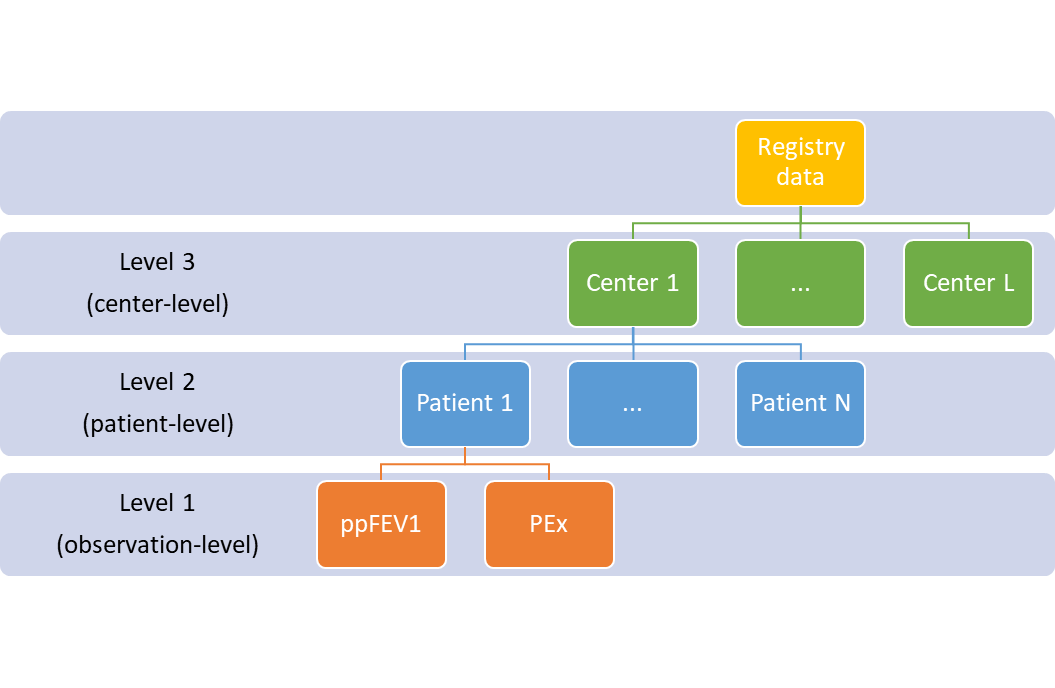
\includegraphics[width=0.65\textwidth]{Figures/Chp1_HDS.png}
\end{figure}
\end{itemize}
\footnotetext[1]{\tiny percent predicted forced expiratory volume in 1 second}
\footnotetext[2]{\tiny pulmonary exacerbation}

\note{For our particular lung disease study, we also have two primary outcomes. ppFEV1 is collected as a longitudinal continuous biomarker to measure the lung function. Pulmonary exacerbation or PEx is a repeated binary event to mark the acute worsening of lung symptoms. Our motivating data is an irregular registry data, which embodies three levels of hierarchy. As displayed in this figure, observed longitudinal outcomes are regarded as the 1st level, which are clustered within patients as the 2nd level, and those patients are from local centers as the 3rd level. We also call such data structure as the multicenter data}
\end{frame}

\begin{frame}{Motivating Data (cont'd)}

\begin{figure}[ht]
    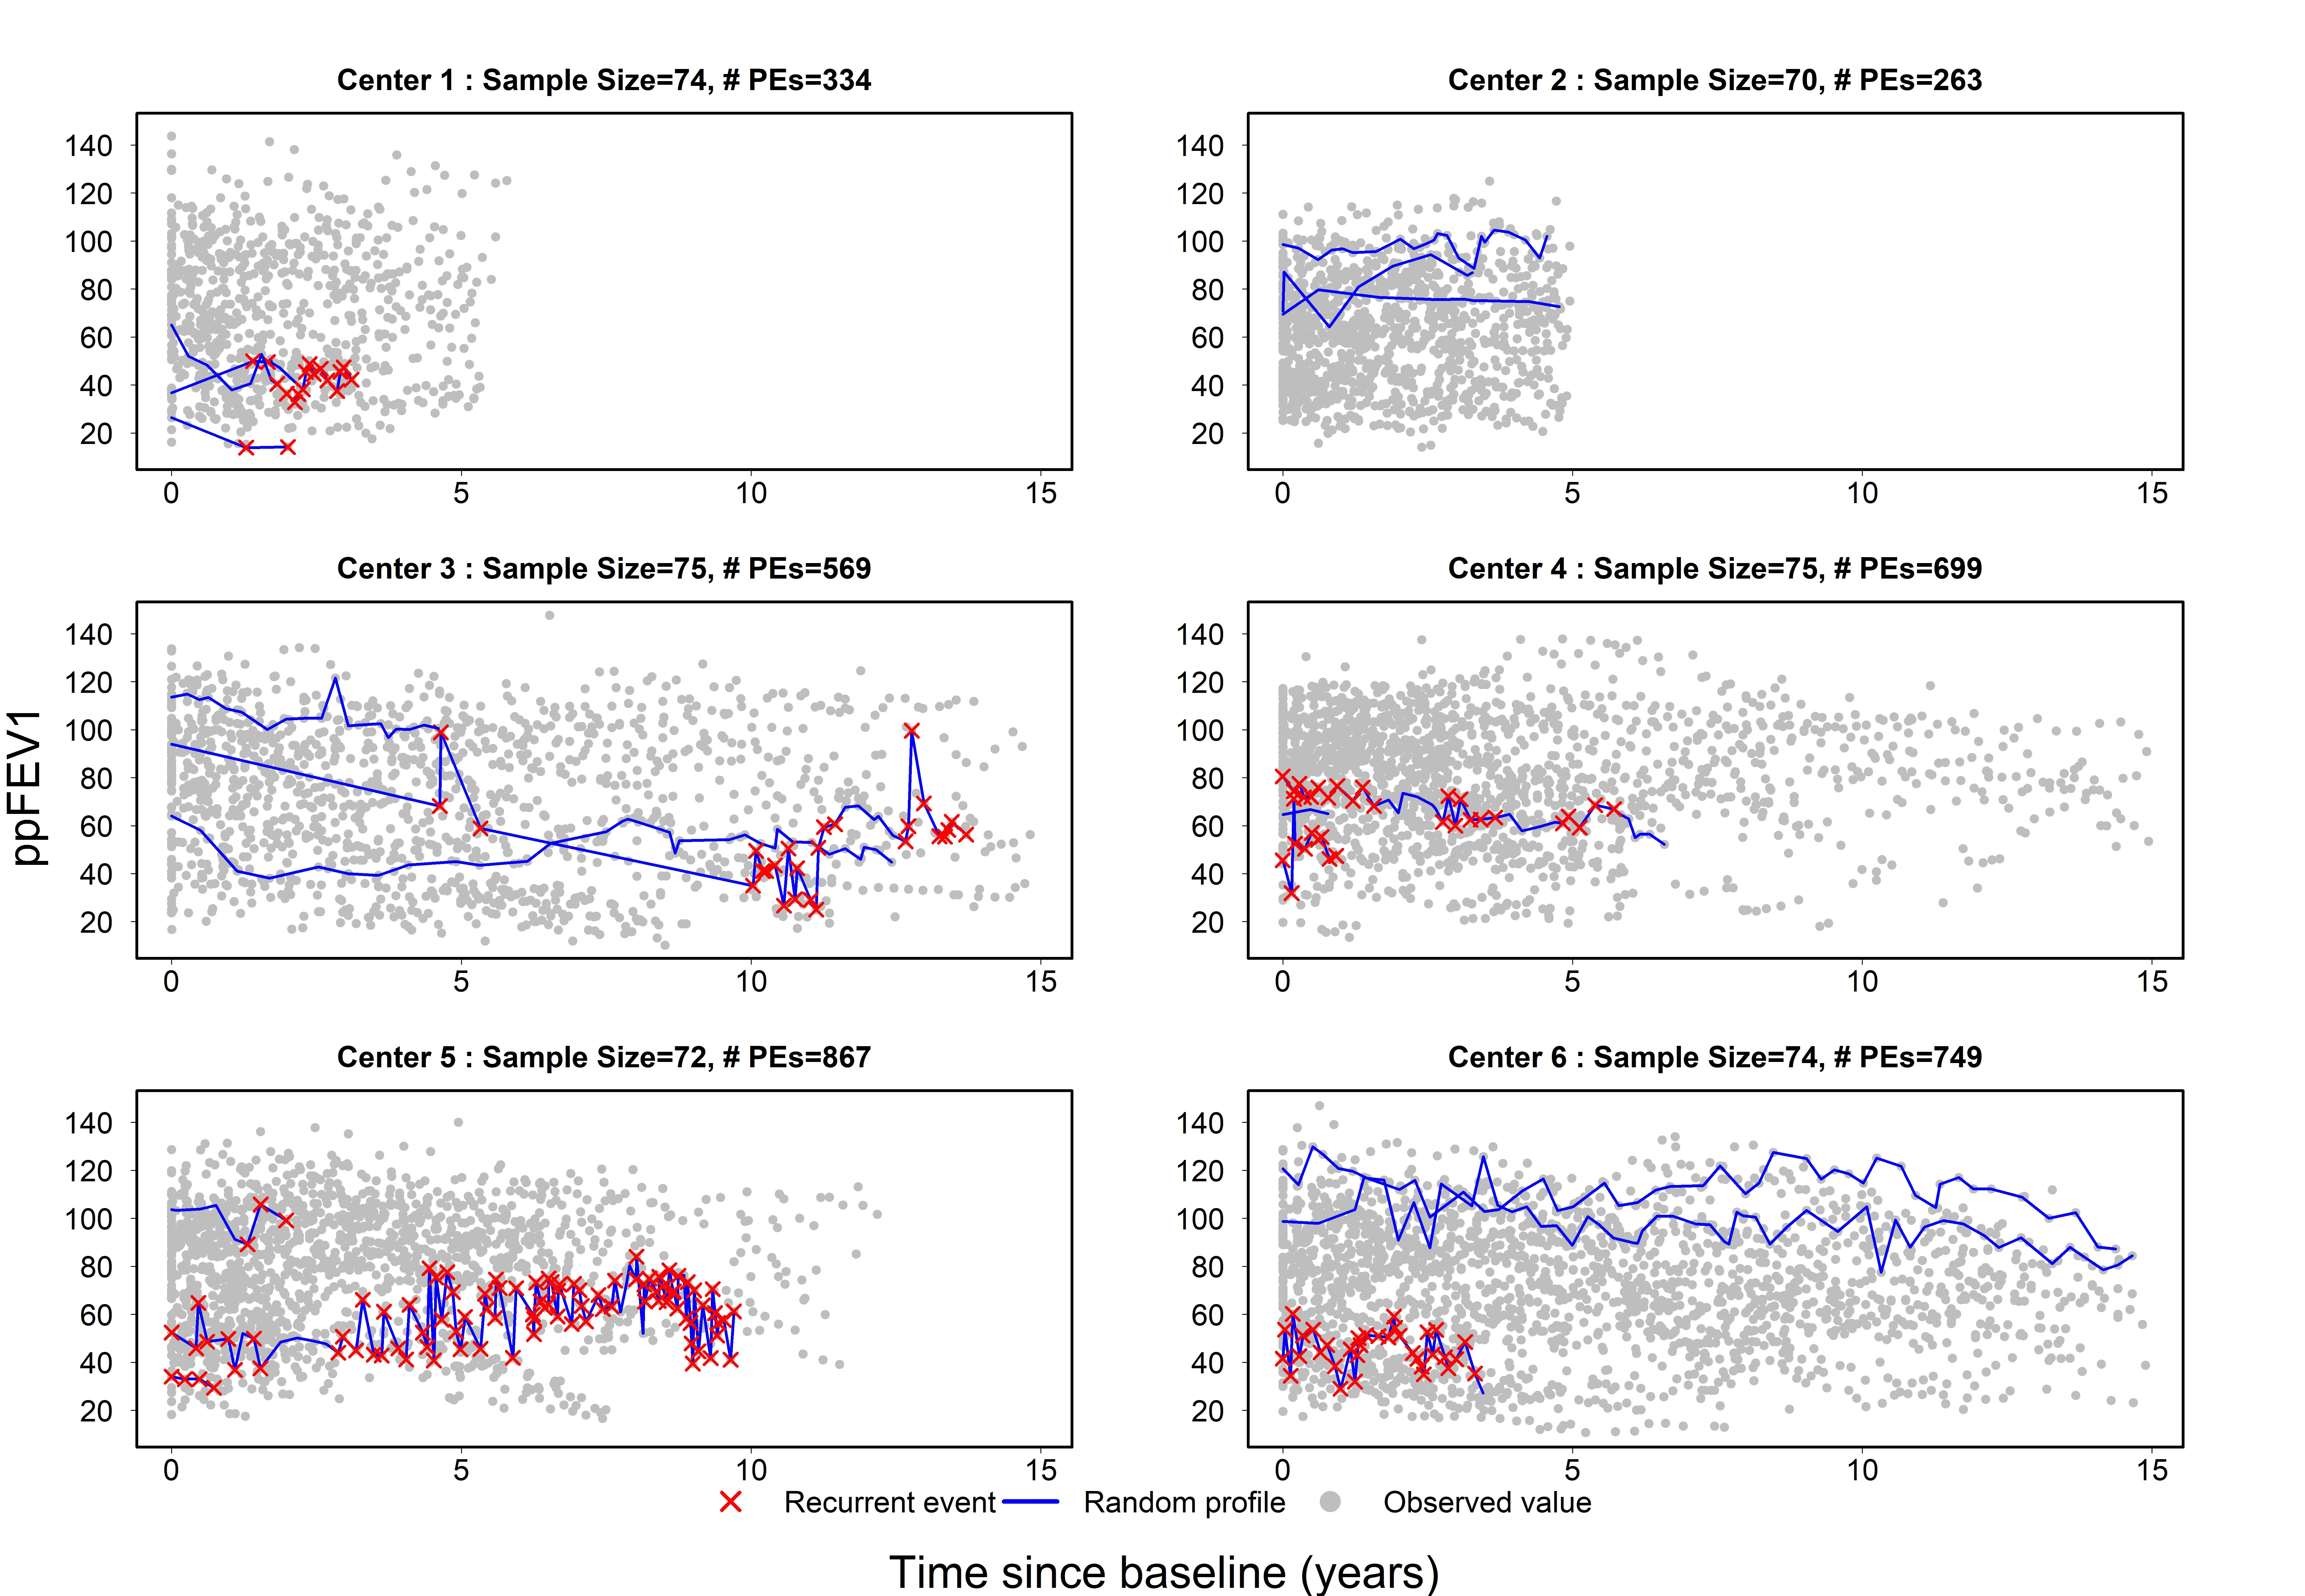
\includegraphics[width=0.9\textwidth]{Figures/Chp3_trajectory.jpg}
\end{figure}
\note{So what does data look like? We plot trajectories against time for six centers. Within each center, three random profiles are displayed with marked recurrent PEx events. This figure implies the non-linear nature of ppFEV1 and also its potential relationship with occurrence of PEx.}
\end{frame}

\begin{frame}
\frametitle{Classical Analysis}
\begin{itemize}
   \item Longitudinal outcomes
    \begin{itemize}
        \item Linear mixed effects (LME)
        \item Generalized linear mixed model (GLMM)
        \item Generalized estimating equation (GEE)
        \item marginal model
        \item ...
    \end{itemize}
   \item Survival outcomes
        \begin{itemize}
            \item Relative risk model (e.g., Cox model)
            \item Accelerated failure time model
            \item Cure frailty model
            \item ...
        \end{itemize}
    \end{itemize}

\note{How can we analyze such two types of outcomes? Methods for the separate analysis are well established in the literature. Specifically, mixed effects models are very popular for longitudinal outcomes by accounting for correlated measurements. With respect to survival outcomes, due to the censoring characteristic, we have well-known Cox model and some others to fit survival outcomes.}    
    
\end{frame}

        
\begin{frame}
\frametitle{Joint Model (JM)}
\small
\begin{columns}
\column{.6\textwidth}
\begin{itemize}
    \item \textcolor{red}{How strong is the association between ppFEV1 and the risk of PEx?} 
   \item Joint modeling {\scriptsize (\cite{Rizopoulos2011})}
     \begin{itemize}
         \item If ppFEV1 is endogenous
         \item If ppFEV1's dropout is nonrandom
     \end{itemize}
    \end{itemize}
 
\column{.4\textwidth}
 \begin{figure}
    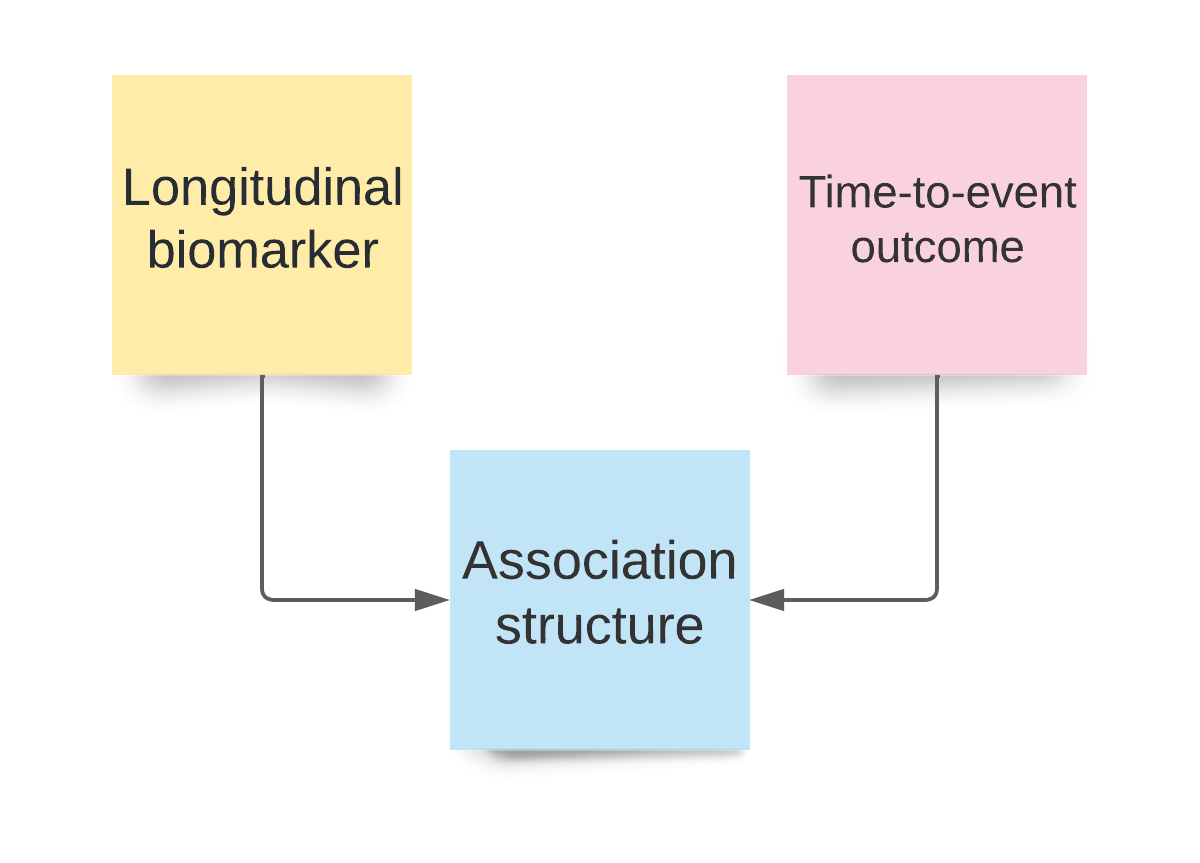
\includegraphics[width=\textwidth]{Figures/Chp1_joint_mod.png}
    % \caption{\scriptsize Joint distribution of the event times and the longitudinal measurements is modeled via a set of random effects that are assumed to account for the associations between these two outcomes}
    \caption{\tiny Rationale of a standard joint model}
\end{figure}
\end{columns}

\note{When it comes to our study question: How strong is the association between ppFEV1 and the risk of PEx? The the separate analysis might be not appropriate any more. Especially, a joint modeling approach is required if
1. ppFEV1 as the time-dependent covariate is endogenous, that is, the occurrence of PEx will affect the future values of ppFEV1.
2. The dropout of ppFEV1 is nonrandom, then the longitudinal and dropout process must be jointly modeled.
Therefore, we propose the joint modeling to study the association b/w ppFEV1 and the risk of PEx. 
The rationale for a standard joint model is displayed here. The latent association structure with a set of random effects is utilized to joint the longitudinal biomarker and the time-to-event outcome. 
}
\end{frame}

\begin{frame}
\frametitle{Extensions}
\begin{itemize}
    \item \textcolor{red}{Categorical longitudinal outcomes}
    \item Multiple longitudinal outcomes
    \item Multiple failure times
    \begin{itemize}
        \item Competing risks
        \item \textcolor{red}{Recurrent events}
        \item Multi-State Process
    \end{itemize}
    \item Heterogenous population
    \begin{itemize}
        \item \textcolor{red}{Stratified relative risk model}
        \item Latent class joint model
    \end{itemize}
\end{itemize}   
\note{Despite the applications of the standard joint model are prevailing. Considerable extensions have been studied as listed here. In today's presentation, our proposed extended joint models will cover these highlights and we will go over them into details shortly.}
\end{frame}


\begin{frame}{Estimation \& Computing}

\begin{itemize}
    \item Frequentist approach
    \item \textbf{Bayesian approach}
\end{itemize}
    \begin{table}[ht]
    \centering
    \caption{\tiny Summary of R package implementation}
    \vspace{-5mm}
    \resizebox{\columnwidth}{!}{
    \begin{threeparttable}
    \begin{tabular}{l|l|c|l}
     \toprule
   \multicolumn{1}{c|}{\textbf{R package}} & 
   \multicolumn{1}{c|}{\textbf{Method}} &
   \multicolumn{1}{c|}{\textbf{Bayesian}} & \multicolumn{1}{c}{\textbf{Reference}}\\
   \toprule
    joineR & Expectation Maximization algorithm & $\times$ & \cite{Philipson2018}\\\hline
    joineRML & Monte Carlo Expectation Maximization algorithm & $\times$ & \cite{Hickey2018a} \\\hline
    JM & Maximum Likelihood Estimation & $\times$ & \cite{Rizopoulos2010} \\\hline
    lcmm & Maximum Likelihood Estimation & $\times$ & \cite{Proust-Lima2022} \\\hline
    \multirow{2}{*}{frailtypack} & \multirow{2}{*}{Maximum Penalized Likelihood Estimation} & \multirow{2}{*}{$\times$} & \cite{Rondeau2012} \\
    &&& \cite{Rondeau2019}\\\hline
    JMBayes & Monte Carlo Markov Chain (MCMC) & \checkmark & \cite{Rizopoulos2016}\\\hline
    JMBayes2 & MCMC & \checkmark & \cite{Rizopoulos2022}\\\hline
    rstanarm \tnote{*} & Hamiltonian Monte Carlo & \checkmark & \cite{Brilleman2018}\\
    \bottomrule
    \end{tabular}
    \begin{tablenotes}
     \item{*} function stan\_jm()
    \end{tablenotes}
     \end{threeparttable}
     }
    \label{tab:chp1_Rpackages}
\end{table}
\note{The estimation and computing techniques for joint modeling can be summarized by Frequentist approach and Bayesian approach. Many powerful R packages are available and listed here. As a fan of R, I skip other softwares, such as SAS, STATA, winBUGs, etc. We favor Bayesian methodology because it is more straightforward for the hierarchical model.}

\end{frame}
  
\begin{frame}{Hamiltonian Monte Carlo (HMC) \& R/Stan}

\begin{itemize}
    
    \item HMC {\scriptsize (\cite{Betancourt2013})}
        \begin{itemize}
            \item Sophisticated but novel MCMC technique
            \item Generate transitions spanning the full marginal variance
            \item Eliminate random walk behavior 
            \item Provide efficient exploration for complex hierarchical models
        \end{itemize}
        
    \item Stan (not an acronym; {\scriptsize \cite{StanManual}})
    \begin{itemize}
        \item Probabilistic programming language
        \item Releases computational constraints of Euclidean HMC
        \item Adapts to No-U-Turn Sampler
        \item R interfaces to Stan
        \begin{itemize}
            \item \textbf{CmdStanr} {\scriptsize (\cite{Gabry2022})}
            \item RStan {\scriptsize (\cite{Rstan2020})}
        \end{itemize}
    \end{itemize}
    
\end{itemize}  
\note{For the computing algorithm, we reply on the Hamiltonian Monte Carlo, short for HMC, which is a sophisticated MCMC method that provides efficient exploration for complex hierarchical models. To achieve posterior estimates through HMC, we adapt to a probabilistic programming language, named Stan. It allows us to build, test and run hierarchical models by specifying the target function. There are two R interfaces to Stan, named cmdstanr and rstan. From our practical experience, cmdstanr as a lightweight interface provides faster convergence and is more compatible to MAC system, thus is preferred. Despite the robustness of existing R packages, we will develop our own R codes and Stan programs to meet the particular need for our multicenter data.}

\end{frame}

\section[Project I: Binary Outcome]{Multilevel Bayesian Joint Model of Longitudinal Continuous and Binary Outcomes}
\setcounter{subsection}{1}

\begin{frame}
\frametitle{}
% \begin{center}
% \textbf{\Large Multilevel Bayesian Joint Model of Longitudinal Continuous and Binary Outcomes}
% \end{center}
\begin{enumerate}
    \item<0> \textbf{Introduction}
    \item \textbf{Multilevel Bayesian Joint Model of Longitudinal and Binary Outcomes}
    \begin{itemize}
        \item Motivation
        \item Model framework
        \item Simulation study \& Motivating data
        \item Discussion
    \end{itemize}
    \item<0> \textbf{Multilevel Bayesian Joint Model of Longitudinal and Recurrent Outcomes}
    \begin{itemize}
        \item Motivation
        \item Model framework
        \item Simulation study \& Motivating data
        \item Discussion
    \end{itemize}
    \item<0> \textbf{Conclusion and Future Work}
\end{enumerate}
\note{For my first project, I will introduce you a multilevel Bayesian joint model that unites longitudinal continuous and binary outcomes. In other words, we regard PEx as the longitudinal binary response.}
% Both center- and individual-level random intercepts are the basis of latent associations between these two submodels. 
\end{frame}

\begin{frame}
\frametitle{Motivation}
\begin{itemize}
    \item Flexible link vs. common links
    \item Non-hierarchical joint model biases
    \item Prognostic utility of the optimal joint model
\end{itemize}
\note{The motivation of this project is threefold: 1) Demonstrate advantages of a flexible link function in a comparison with three common link functions; 2) Quantify biases caused by a non-hierarchical joint model; 3) Evaluate predictive performance of the optimal joint model}
\end{frame}


\begin{frame}
\frametitle{Model Framework}
\tiny
Let $l,i,j$ denote center, patient, time point with $l=1,\dots,L; i=1, \dots,n_l; j=1,\dots,n_{li}$, respectively.
\footnotesize
\begin{itemize}
    \item \textbf{Longitudinal continuous submodel}
    \begin{align}
        \mbox{LME\footnotemark:} Y_{lij}=\bm{X}_{li}(t_{lij})\bm{\alpha}+b_l+U_{li}+W_{li}(t_{lij}) + \epsilon_{lij}
    \end{align}
where $b_l \sim N(0,\sigma^2_b)$, $U_{li} \sim N(0, \sigma^2_u), \epsilon_{lij} \sim N(0, \sigma^2), \bm{b} \ind \bm{U} \ind \bm{\epsilon}$. \newline\newline The stochastic Gaussian process $\bm{W}_{li}(t)$ follows $N(\bm{0},\Sigma_w)$ with exponential covariance
\begin{align}
Cov(W_{li}(t),W_{li}(s))=\tau^2 exp \big (-|t-s| \cdot \rho \big)
\end{align}

    \item \textbf{Longitudinal binary submodel}
    \begin{align}
    \mbox{GLMM\footnotemark}: Pr(R_{lij}=1)=g^{-1}\big(\bm{V}_{li}(t_{lij})\bm{\beta}+\rho_1 b_l + \rho_2 U_{li}; r_l\big)
    \end{align}
where $\rho_1, \rho_2 \in (-1,1)$, $g(\cdot)$ is some known link function. 

\end{itemize}
\footnotetext[3]{\tiny Linear Mixed Effect}
\footnotetext[4]{\tiny Generalized Linear Mixed Model}
\note{Here are some notations. Let $l,i,j$ denote center, patient, time point, respectively and we adapt to a shared parameter joint model.
In the longitudinal continuous submodel, we fit ppFEV1 with LME. let $Y$ denote observed values for ppFEV1, $X$ is the design matrix with corresponding unknown coefficient $\alpha$. Random intercept $b$ is for center and random intercept $U$ is for patient, both with the assumption of independent normal distribution. The measurement error is also assumed to follow an iid normal distribution. The Gaussian process $W$ describes how individual lung function varies over time in the form of an exponential correlation with parameter $\tau, \rho$.
In the longitudinal binary submodel, we fit PEx with GLMM. That is, the probability of an event equals to the inverse of some known link function, which is composed of fixed effects and shared random components. Parameters $\rho_1$ and $\rho_2$ measure the strength of the association between these two submodels. 
}
\end{frame}

\begin{frame}
\frametitle{Symmetric Power Link Family {\scriptsize (\cite{Jiang2013})}}
\begin{equation} \label{eq:ch2_Fsp}
  F_{sp}(x;r)=F_0^r(\frac{x}{r})I_{(0,1]}(r)+\big[1-F^{1/r}_0(-rx)\big]I_{(1,+\infty)}(r),    
\end{equation}
\footnotesize
where covariate $x \in (-\infty,+\infty)$, power parameter $r \in (0, +\infty)$, $I_A(r)=1$, when $r \in A$ or $I_A(r)=0$, otherwise.

\begin{itemize}
    \item symmetric power logit ($F_{splogit}$)
    $$F_0=F_{\mbox{logistic}}(x|\mu=0, s=1)= \frac{1}{1+exp(-x)}$$
    \item symmetric power exponential power ($F_{spep}$)
    $$F_0=F_{\mbox{laplace}}(x|\mu=0, b=1)=\frac{exp(x)}{2}I_{(-\infty,0)}(x)+\big(1-\frac{exp(x)}{2}\big)I_{[0, +\infty)}(x)$$
\end{itemize}

\note{For the choice of link function, we prefer a symmetric power link as expressed in the Equation 4. Because such link function allows for flexible skewness of response, which is controlled by the power parameter $r$. Particularly, we have splogit if $F_0$ follows a standard Logistic distribution, or we have spep if $F_0$ follows a standard laplace distribution. We will demonstrate the flexibility of splogit compared to the common link choices and comparison between splogit and spep shortly.}
\end{frame}


\begin{frame}
\frametitle{Conditional Independence Assumption}
Random effects explain all the interdependence: 
\newline
\begin{itemize}
    \item Repeated measurements/events in each submodel are independent of each other
    \item Two submodels are conditionally independent
\end{itemize}
\note{A key assumption for joint modeling is the conditional independence, which means that random effects will explain all the interdependence. So that: read slide. This key assumption will apply to both of our projects.}
\end{frame}

\begin{frame}
\frametitle{Joint Posterior Distribution}
\footnotesize
\begin{flalign}
\pi(\bm{\Psi},\bm{b},\bm{U},\bm{W}|\mathcal{D}) 
& \propto \pi(\mathcal{D},\bm{b},\bm{U},\bm{W}|\bm{\Psi}) \pi(\bm{\Psi})&&\\\nonumber
& \propto \pi(\mathcal{D}|\bm{b},\bm{U},\bm{W},\bm{\Psi}) \pi(\bm{b}|\bm{U},\bm{W},\bm{\Psi})\pi(\bm{U}|\bm{W},\bm{\Psi})\pi(\bm{W}|\bm{\Psi})\pi(\bm{\Psi})&&\\\nonumber
& \propto \pi(\bm{Y},\bm{R}|\bm{b},\bm{U},\bm{W},\bm{\Psi}) \pi(\bm{b}|\bm{\Psi}) \pi(\bm{U}|\bm{\Psi}) \pi(\bm{W}|\bm{\Psi}) \pi(\bm{\Psi})&&\\\nonumber
& \propto \prod_{l=1}^{L}\prod_{i=1}^{n_l}I(\bm{Y}_{li},\bm{R}_{li}|b_{l}, U_{li}, \bm{W}_{li}, \bm{\Psi}) \pi(b_l|\sigma_b) \pi(U_{li}|\sigma_u) \pi(\bm{W}_{li}|\tau,\rho)\pi(\bm{\Psi})&& 
\end{flalign}
where $\mathcal{D}$ denotes observed data, $\bm{\Psi}$ represents unknown mutually independent parameters. By the assumption of conditional independence: 
$$\bm{I}(\bm{Y}_{li},\bm{R}_{li}|b_l,U_{li},\bm{W}_{li},\bm{\Psi})= \bm{I}_1(\bm{Y}_{li}|b_l,U_{li},\bm{W}_{li},\bm{\Psi}) \bm{I}_2(\bm{R}_{li}|b_l,U_{li},\bm{\Psi})$$

\note{With conditional independence assumption, it is easier for us to derive the joint posterior distribution by Bayesian inference.}

\end{frame}

\begin{frame}{Prior Distributions}

\begin{table}[H]
\caption{Prior specifications}
 \vspace{-5mm}
\resizebox{\columnwidth}{!}{
\begin{threeparttable}
  \begin{tabular}{cccc}
    \toprule
Priors & Simulation Study 1 & Simulation Study 2 & Motivating Data \\
 \midrule 
   $\bm{\alpha,\beta}$ &  $N(0,10\bm{I})$ & $N(0,100\bm{I})$ & $N(0,100\bm{I})$ \\
   $\sigma_b$ & $\mbox{Half-Cauchy}(0,5)$ & $\mbox{Half-Cauchy}(0,5)$ & $\mbox{Half-Cauchy}(0,5)$ \\
  $\sigma_u$ & $\mbox{Truncated }\mbox{student-t}(1,0,5)$ & $\mbox{Half-Cauchy(0,5)}$ & $\mbox{Half-Cauchy(0,5)}$ \\
  $\sigma$ & $\mbox{Half-Cauchy}(0, 2.5 \cdot sd)$  &  $\mbox{Half-Cauchy}(0, 2.5 \cdot sd)$ & $\mbox{Half-Cauchy}(0, 2.5 \cdot sd)$ \\
    $\rho_1, \rho_2$ & $\mbox{Uniform}(-1, 1)$ & $\mbox{Uniform}(-1, 1)$ & $\mbox{Uniform}(-1, 1)$ \\
    $\bm{r}$ & $\mbox{Exponential}(1)$ & $\mbox{Gamma}(2,2)$ & $\mbox{Exponential}(1)$ \\
   \hline
   $\tau$ & - & $\mbox{Truncated } N(0, 5)$ & $\mbox{Truncated } N(0, 5)$ \\
   $\rho$ & - & $\mbox{Inv-Gamma}(2, 1)$ & $\mbox{Inv-Gamma}(2,1)$\\
    \bottomrule
  \end{tabular}
   \begin{tablenotes}[para]
    \scriptsize
    Note: sd=standard deviation of longitudinal residuals; N(location,scale); Half-Cauchy(location,scale); student-t(df,location,scale); Exponential(rate); Gamma(shape,rate); Inv-Gamma(shape,scale);
    \end{tablenotes}
  \end{threeparttable}
  }
\end{table}

\note{For prior distributions, we subjectively set non-informative or weakly informative priors based on many references.
% So they are quite subjective. 
%For scale parameters, like $\sigma_b, \sigma_u, \sigma$, we favor half-cauchy or student-t distribution over the common choice of inverse gamma to capture smaller values.
}
\end{frame}


\begin{frame}{Computation}

\begin{table}[H]
\footnotesize
\begin{threeparttable}
 \begin{tabular}{lccc}
    \toprule
 HMC & Simulation Study 1 & Simulation Study 2 & Motivating Data \\
 \midrule 
 Interface to Stan & cmdstanr & rstan & rstan \\
 Post-warmup \tnote{+} & 4000 & 4000 & 5000 \\
 Chains & 2 & 2 & 2\\
    \bottomrule
  \end{tabular}
\begin{tablenotes}
\tiny
\item{\textsuperscript{+}} Converged samplings validated by $\hat{R}=1$ (\cite{Gelman1992})
\end{tablenotes}
\end{threeparttable}
\end{table}
\note{The posterior samplings are carried out through HMC by Stan as summarized in the table.}
\end{frame}

\begin{frame}
\frametitle{Dynamic Individual Prediction}
\footnotesize
\begin{itemize}
    \item Best linear unbiased predictor (BLUP)
    \item Predict for a new patient from the existing center
    \begin{align}
   & E\big(U_{li'}|\bm{Y}_{li'},b_l, \bm{\phi},\bm{\alpha}\big)  = \sigma_u^2\bm{K}^T_{li'}\big(\bm{V}_{li'}(\bm{\phi})\big)^{-1} (\bm{Y}_{li'}-\bm{X}_{li'}\bm{\alpha}-b_l\bm{K}_{li'})\label{chp2:eq4} \\
   & E\big(W_{li'}(t_{li'j}\big)|\bm{Y}_{li'},b_l, \bm{\phi},\bm{\alpha})  =  \tau^2\bm{F}^{j^T}_{li'}\big(\bm{V}^j_{li'}(\bm{\phi})\big)^{-1}  (\bm{Y}^j_{li'}-\bm{X}^{j}_{li'}\bm{\alpha}-b_l\bm{K}^j_{li'}) 
\end{align}
\scriptsize
where $\bm{K}$ is a column vector of ones, $\bm{V}(\bm{\phi})=\sigma_u^2\bm{J}+\tau^2\bm{R}+\sigma^2\bm{I}$, $\bm{J}$ is all ones matrix, $\bm{R}$ is an exponential correlation matrix, $\bm{I}$ is an identity matrix and $\bm{F}^j=(exp(-|t_1-t_j|) \cdot \rho,\dots,exp(-|t_j-t_j|) \cdot \rho)^T$

\footnotesize
\item Forecast for an existing patient
\begin{align}
  E\big(W_{li}(t_{lij}+u)|\bm{Y}^j_{li},b_l, U_{li},\bm{\phi}, \bm{\alpha}\big)  =  \tau^2\bm{F}^{{j,u}^T}_{li}\big(\bm{G}^j_{li}(\bm{\phi})\big)^{-1}(\bm{Y}^j_{li}-\bm{X}^{j}_{li}\bm{\alpha}-b_l\bm{K}^j_{li}-U_{li}\bm{K}^j_{li}) 
\end{align}
\scriptsize
where $\bm{G}^j(\bm{\phi})=\tau^2\bm{R}^j+\sigma^2\bm{I}^j$ denotes variance-covariance matrix of $\bm{Y}^j$ (response history up to an observed time point $j$)

\end{itemize}

\note{Now we come to the method of individual prediction. We adapt to the best linear unbiased predictor (BLUP) through the property of conditional multivariate normal distribution. As we assume the new patient is from existing center, we only need to derive the expectation for random intercept U and time-continuous random variable W by Equation 6 and 7. To forecast for an existing patient, we only need to predict W at a future time by assigning a time window $u$. Whenever a new response at future time $t_{lij}+u$ becomes available, the prediction will be dynamically updated. Practically, we will replace all unknown parameters with the posterior mean estimates to achieve the empirical BLUP.}

\end{frame}

\begin{frame}
\frametitle{Model Selection}
\begin{itemize}
\footnotesize
    \item Watanabe-Akaike information criterion (WAIC, {\scriptsize (\cite{Watanabe2010})})

\begin{equation}
    \begin{split}
    \mbox{WAIC}=-2\Big \{\sum_{i=1}^{n}log\big(p_{post}(y_i|\theta)\big)-\sum_{i=1}^{n}\mbox{var} \Big (log\big( p_{post}(y_i|\theta)\big) \Big ) \Big \}
    \end{split}
\end{equation}
    \item Invariant to reparameterizations contrary to DIC\footnotemark {\scriptsize (\cite{Spiegelhalter2002})}
    \item Computed by loo::waic()
    \item The smaller the better
\end{itemize}
\footnotetext[5]{\tiny Deviance Information Criterion}
\note{We prefer WAIC as the model selection criterion. Because it is a full Bayesian approach for estimating the out-of-sample expectation by marginalizing over posterior distribution, thus is invariant to reparameterizations contrary to the DIC. Practically, the computed WAIC can be easily achieved by the waic function from R package \emph{loo}. The model with the smaller WAIC indicates the better goodness of fit.}
%(by extracting pointwise log-likelihood values from the posterior samplings)
\end{frame}

\begin{frame}
\frametitle{Simulation Study 1}
Compare flexible link (splogit) with common links:
\newline
\scriptsize 
\noindent
 \begin{align}
& \left \{\begin{array}{ll}
  g^{-1}_{logit}(x) = F_{logit}(x)= [1+exp(x)]^{-1}\\[10pt]
  g^{-1}_{probit}(x) = F_{probit}(x)= \Phi(x), \mbox{where $\Phi$ is standard normal cdf}\\[10pt] 
  g^{-1}_{cloglog}(x) = F_{cloglog}(x)= 1-e^{-e^x}\\[10pt]
  g^{-1}_{splogit}(x,r) = F_{splogit}(x,r)=[1+exp(\frac{x}{r})]^{-r}I_{(0,1]}(r)+\big\{1-[1+exp(-rx)]^{-\frac{1}{r}}\big\} I_{(1,+\infty)}(r)
\end{array}\right.
\end{align}

\note{So far, we have talked about our model framework, including flexible link function, Bayesian inference, individual prediction and model selection. Now, we move forward to our simulation studies. Our first simulation is designed to explore the flexibility of splogit in a comparison with three common links that you might be familiar with, logit, probit and cloglog.}

\end{frame}

\begin{frame}
\frametitle{Simulation 1: Model Structures}
\footnotesize
\begin{align*}
\mbox{logit-JM} & \left \{\begin{array}{ll}
        Y_{lij}= \alpha_0 + x_{li1}\alpha_1 + x_{li2}\alpha_2 + b_l + U_{li} + \epsilon_{lij} \\
       \mbox{Pr}(R_{lij}=1)=F_{logit}(\beta_0 + \beta_1 t_{lij} + \rho_1 b_l + \rho_2 U_{li}) \\
\end{array}\right. \\
\mbox{probit-JM} & \left \{\begin{array}{ll}
       Y_{lij}= \alpha_0 + x_{li1}\alpha_1 + x_{li2}\alpha_1+b_l+U_{li} + \epsilon_{lij} \\
       \mbox{Pr}(R_{lij}=1)=F_{probit}(\beta_0 + \beta_1 t_{lij} +\rho_1 b_l + \rho_2 U_{li}) \\
\end{array}\right. \\
\mbox{cloglog-JM} & \left \{\begin{array}{ll}
       Y_{lij}= \alpha_0 + x_{li1}\alpha_1 + x_{li2}\alpha_1+b_l+U_{li} + \epsilon_{lij} \\
       \mbox{Pr}(R_{lij}=1)=F_{cloglog}(\beta_0 + \beta_1 t_{lij} + \rho_1 b_l + \rho_2 U_{li}) \\
        \end{array}\right.\\
\mbox{\bf splogit-JM} & \left \{\begin{array}{ll}
       Y_{lij}= \alpha_0 + x_{li1}\alpha_1 + x_{li2}\alpha_1+b_l+U_{li} + \epsilon_{lij} \\
       \mbox{Pr}(R_{lij}=1)=F_{splogit}(\beta_0 + \beta_1 t_{lij} + \rho_1 b_l + \rho_2 U_{li};\textcolor{red}{r_l}) \\
       \end{array}\right.        
\end{align*}
\note{Then we simulate the multicenter data through true splogit-JM to fit following 4 models for 50 replicates. All models shared the same submodel for Y, and the differences exist in the link function we applied. }  
% however, only splogit model incorporates center-specific power parameter to control the different skewness of response from each center.
\end{frame}

\begin{frame}
\frametitle{Simulation 1: WAIC}
\footnotesize
\begin{table}[H]
\caption{\scriptsize Model comparisons over simulated data sets for 50 replicates}
 \begin{threeparttable}
  \begin{tabular}{llll}
  \toprule
 Fitted Model \hspace*{5mm} & $\mbox{WAIC}$ \tnote{a} \hspace*{4mm} & $\mbox{WAIC}_1$ \tnote{b}  \hspace*{4mm}  & $\mbox{WAIC}_2$ \tnote{c}  \hspace*{4mm}\\
 \midrule
   logit-JM & 2239.93 & 1807.16 & 432.77 \\
  
   probit-JM & 2244.44 & 1807.49 & 436.95 \\
  
   cloglog-JM & 2272.57  & 1808.24 & 464.33 \\
   
   \bf splogit-JM & \bf 2203.00 & \bf 1806.37 & \bf 396.63 \\
    \bottomrule
  \end{tabular}
  \begin{tablenotes}[para]
    \tiny
    Model in boldface: true model; \item[a] Joint model; \item[b] Longitudinal continuous submodel; \item[c] Longitudinal binary submodel
    \end{tablenotes}
    \end{threeparttable}
\end{table}
\note{Averaged WAIC is summarized in this table. The smallest value of WAIC2 validates the great flexibility induced by center-specific power parameter than common link choices. Therefore, a flexible link function is preferred for the multicenter data.}
\end{frame}

\begin{frame}
\frametitle{Simulation 1: Results}
\begin{figure}[H]
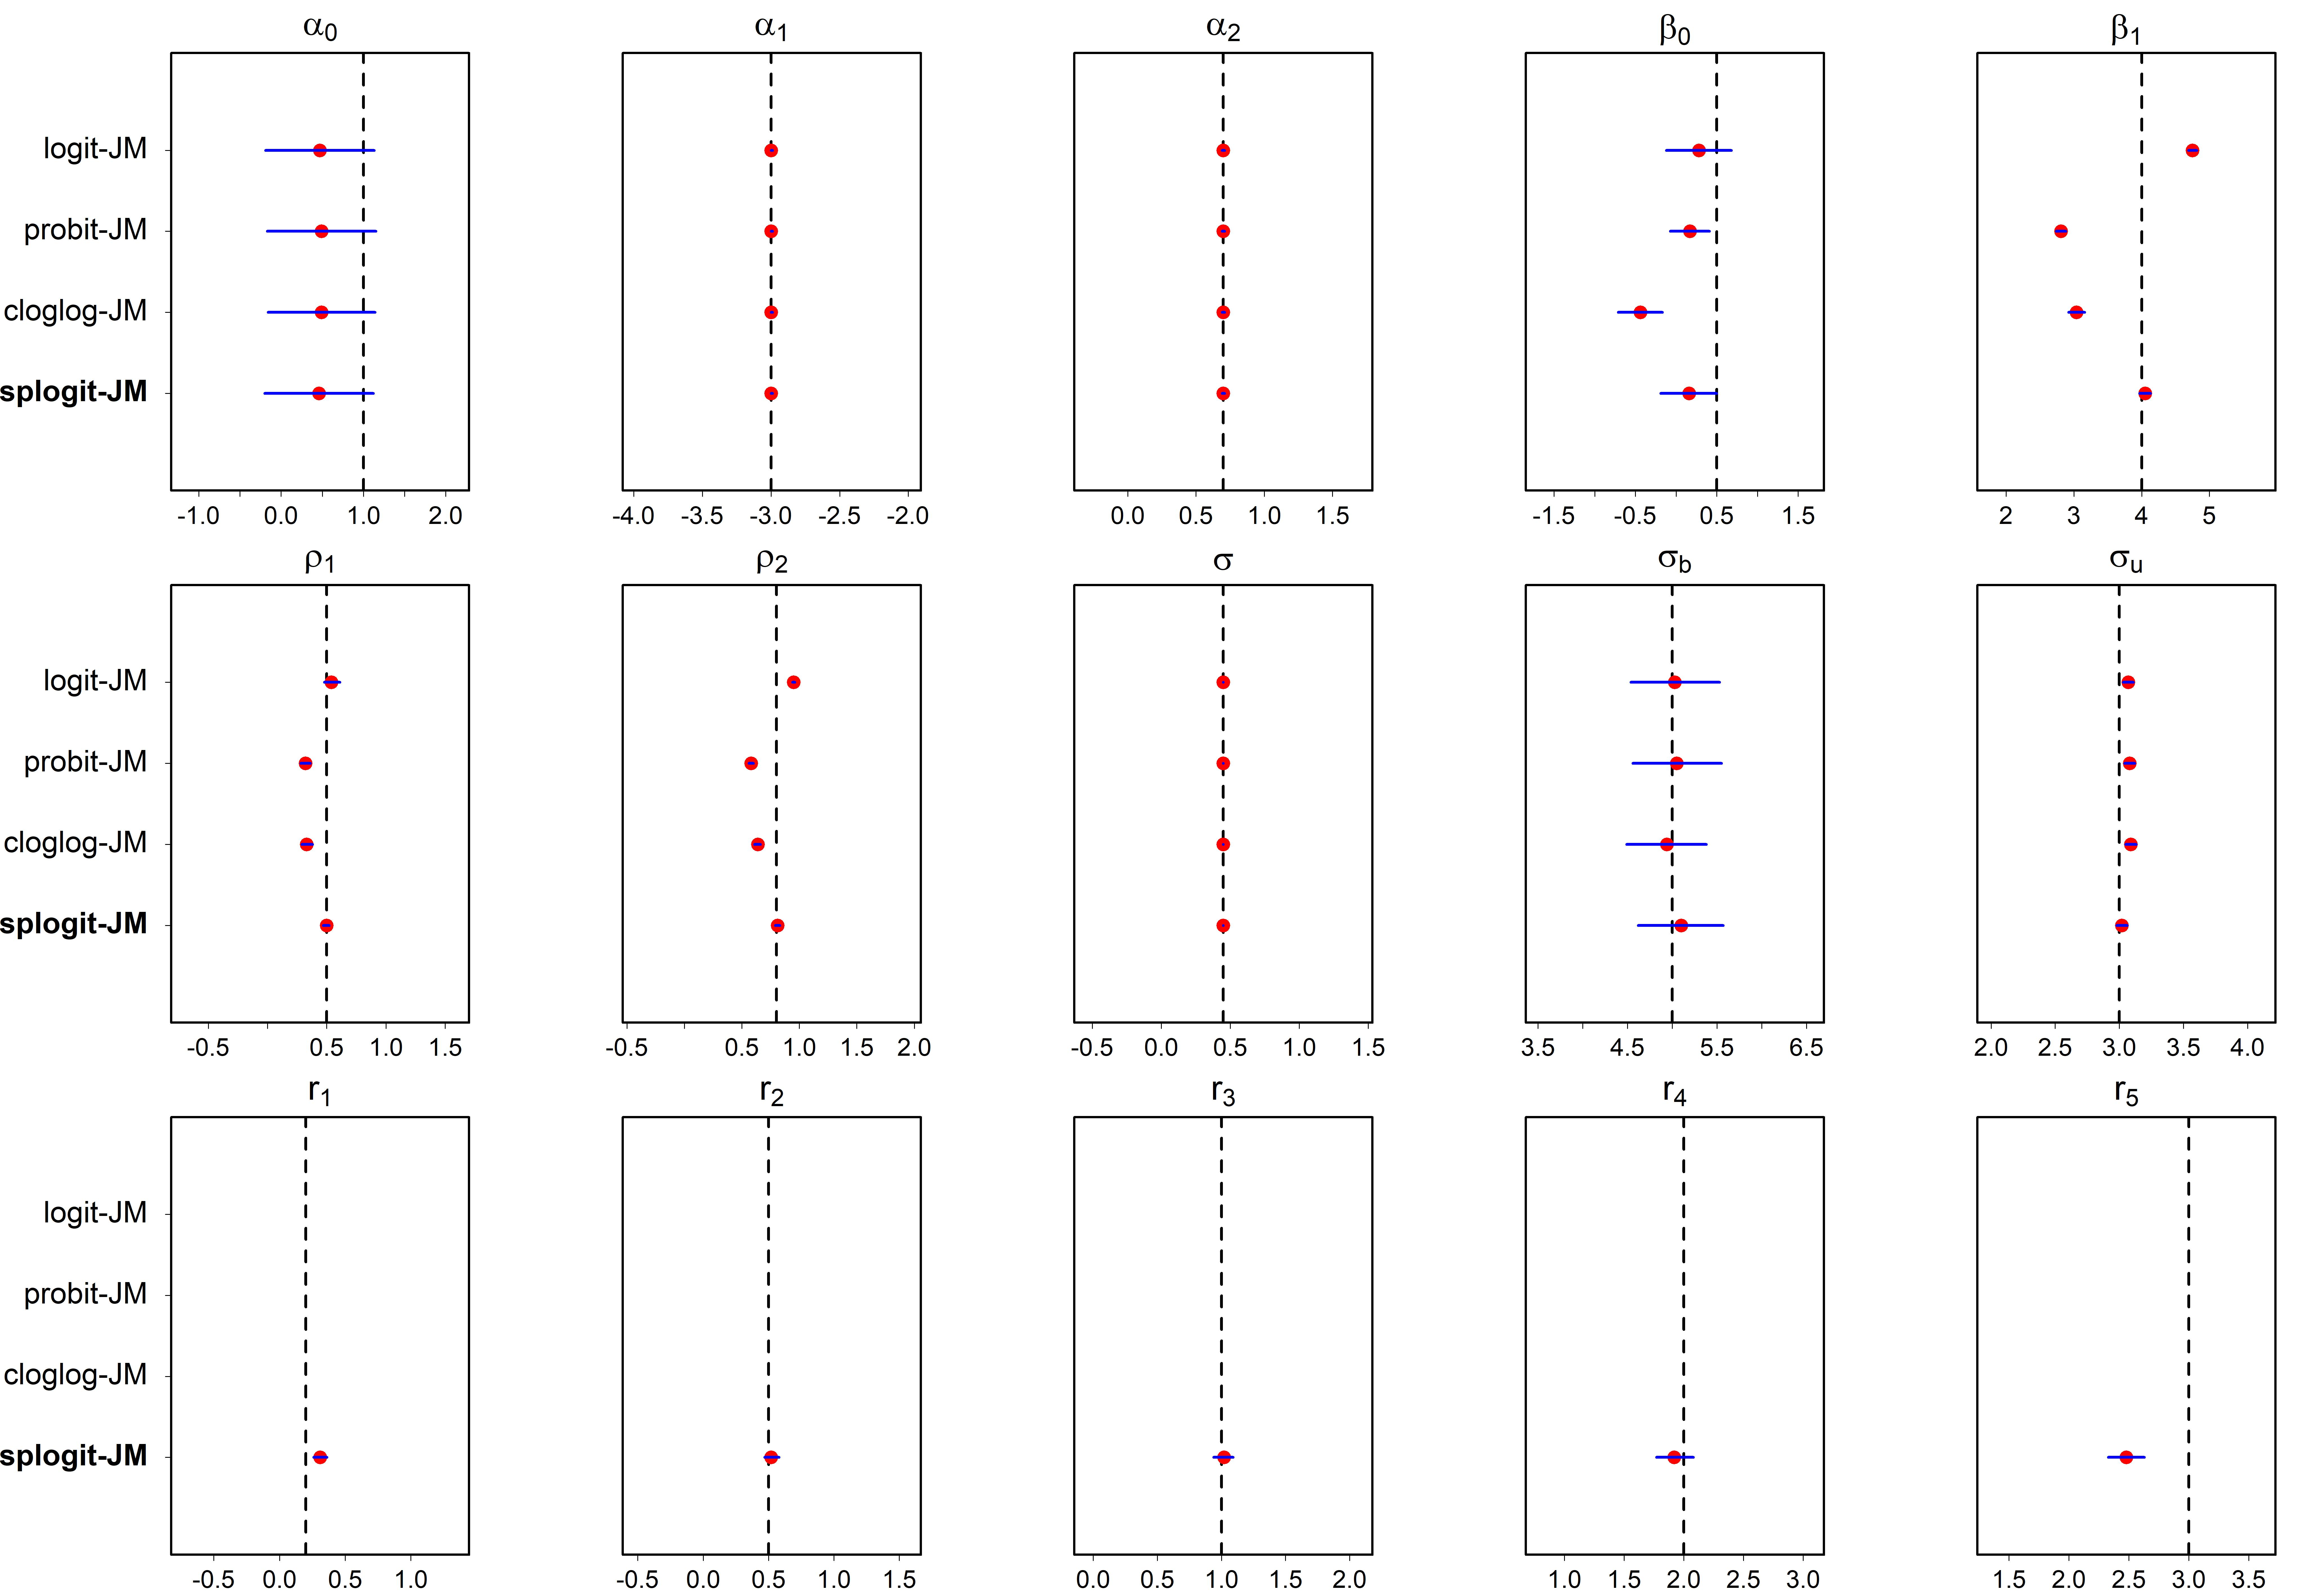
\includegraphics[width=0.80\textwidth]{Figures/Chp2_SIM_SPLOGIT_A.jpg}
\caption{\tiny Averaged \textcolor{red}{posterior mean (red dot)} with \textbf{true model (boldface)}, true value (dashed line) and \textcolor{blue}{95\% confidence interval (blue line)} for 50 replicates via CmdStanr.}
\end{figure}
\note{We visualize the simulation results here. We expect posterior mean estimate denoted by red dot to be close to true values denoted by dashed line. We can tell the reasonable performance of our true model, but estimates for $\alpha_0$ and $r_5$ can be further improved by more replicates. If we take a close look at $\beta_1$, our proposed model performs much better than the other three models in recovering the true value. }
\end{frame}

\begin{frame}
\frametitle{Simulation Study 2}
\begin{figure}[H]
\centering
\begin{columns}
        \column{0.55\textwidth}
        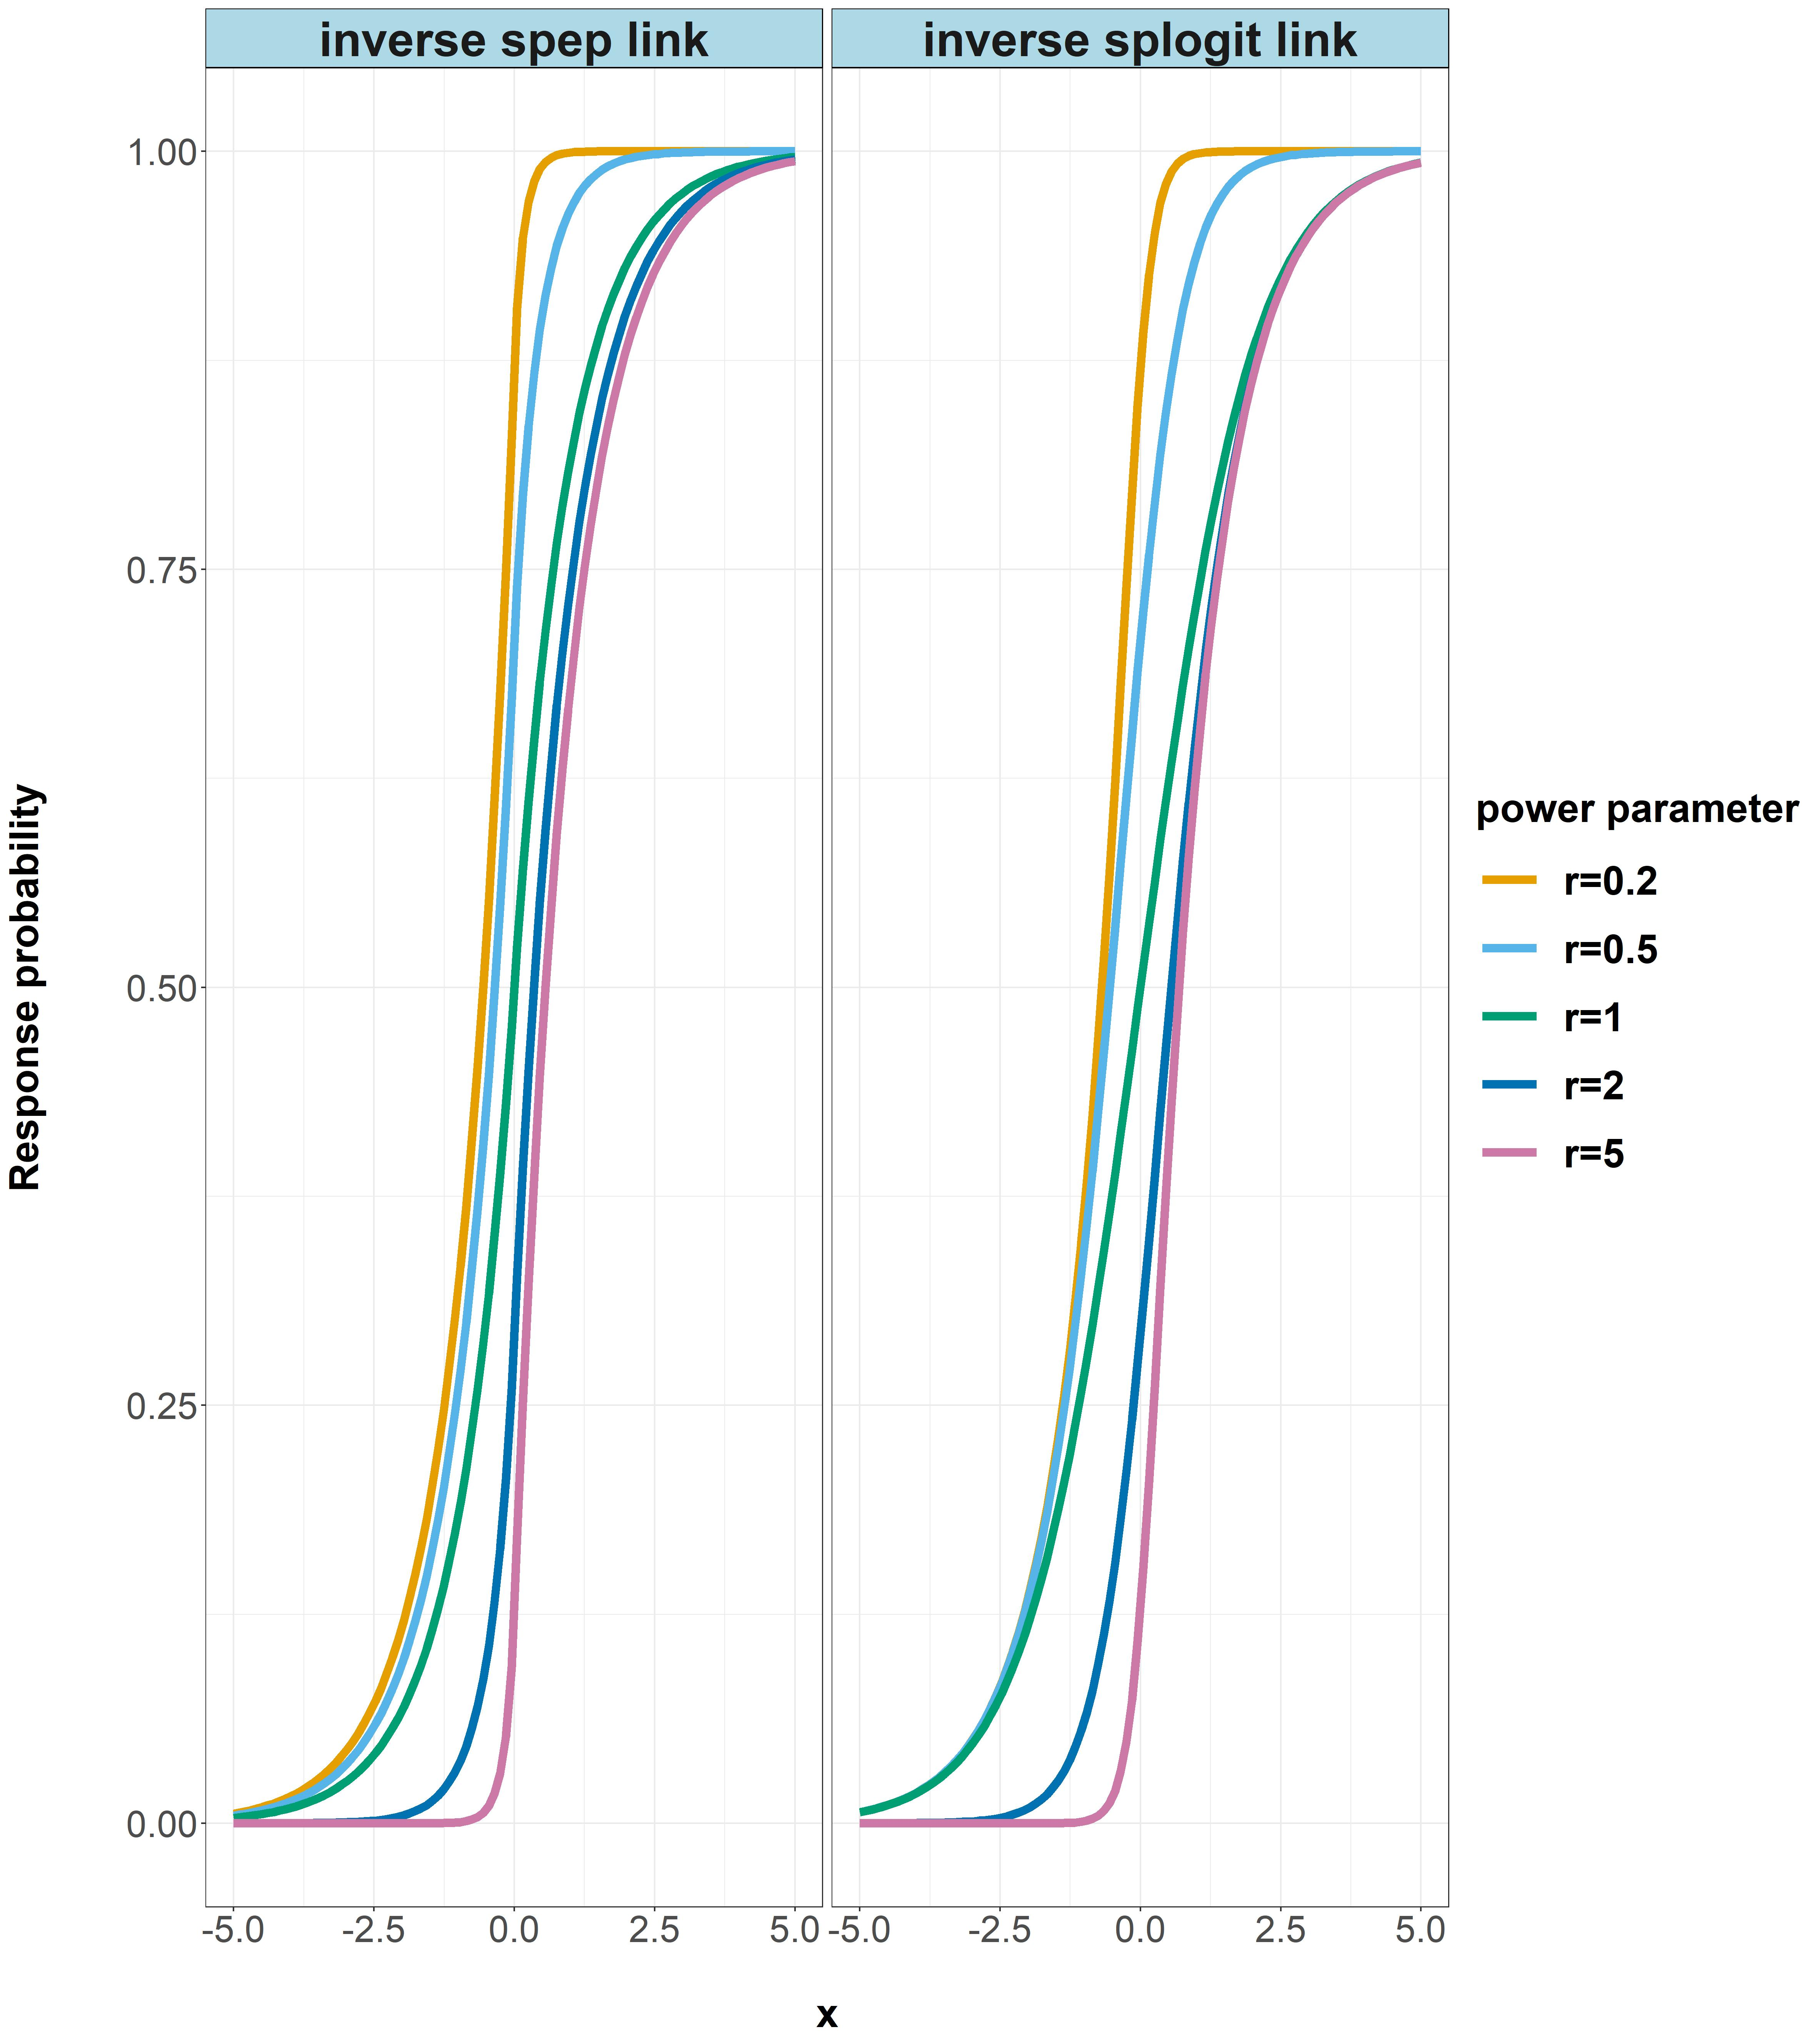
\includegraphics[width=\textwidth]{Figures/Chp2_cdf_link.jpg}
        \column{0.45\textwidth}
     
        \begin{itemize}
            \item spep
            \begin{itemize}
                \item flexible range of skewness
                \item adjustment of tail behavior
            \end{itemize}
            \item splogit
            \begin{itemize}
                \item logit link when power parameter $r=1$
            \end{itemize}
        \end{itemize}
        
        
\end{columns}

\end{figure}
\note{As we see from the previous simulation, a flexible link function is recommended. Then we may question which flexible link to choose. From the figure, we tell that spep provides more flexible range of skewness and adjustment of tail behavior than the sploigt. Therefore, we choose spep as the flexible link function in the following analysis.}
\end{frame}


\begin{frame}
\frametitle{Simulation Study 2: Model Structures}
Compare the performance of proposed joint model with naive joint models: 
 \begin{align*}
& \mbox{JM}_1 \left \{\begin{array}{ll}
        Y_{lij}= U_{li} + \epsilon_{lij} \\
       \mbox{Pr}(R_{lij}=1)=F_{spep}(\beta_0+\beta_1t_{lij}+ \rho_2 U_{li};r) \\
\end{array}\right. \\
& \mbox{JM}_2 \left \{\begin{array}{ll}
        Y_{lij}=b_l + U_{li} + \epsilon_{lij}\\
       \mbox{Pr}(R_{lij}=1)=F_{spep}(\beta_0+\beta_1t_{lij}+\rho_1 b_l + \rho_2 U_{li};r) \\
\end{array}\right. \\
& \mbox{JM}_3 \left \{\begin{array}{ll}
       Y_{lij}=b_l + U_{li} + \epsilon_{lij} \\
       \mbox{Pr}(R_{lij}=1)=F_{spep}(\beta_0+\beta_1t_{lij}+\rho_1 b_l + \rho_2 U_{li};r_l) \\
        \end{array}\right.\\
& \mbox{\bf JM}_4 \left \{\begin{array}{ll}
        Y_{lij}=b_l + U_{li} + \textcolor{red}{W_{lij}} + \epsilon_{lij} \\
       \mbox{Pr}(R_{lij}=1)=F_{spep}(\beta_0+\beta_1t_{lij}+\rho_1 b_l + \rho_2 U_{li};\textcolor{red}{r_l}) \\
       \end{array}\right.        
\end{align*}

\note{Then with the aim to explore the performance of our proposed joint model, we implement four scenarios. Specifically, JM1 is constructed as a non-hierarchical joint model, JM2 is a hierarchical joint model but with a common power parameter, JM3 is very close to the proposed JM4, but without the Gaussian process, so we call it Naive LME}
\end{frame}

\begin{frame}
\frametitle{Simulation 2: WAIC}

\begin{table}[ht]
\caption{\footnotesize Model comparisons over simulated data sets for 50 replicates} \label{tab:chp2_sim}
\footnotesize
 \begin{threeparttable}
\begin{tabular}{lllllll}
    \toprule
  Fitted Model &
 $\mbox{WAIC} \tnote{a}$ & $\mbox{WAIC}_1 \tnote{b}$ & $\mbox{WAIC}_2 \tnote{c}$ \\
 \midrule 
   Non-hierarchical (spep-$\mbox{JM}_1$) & 
                9256.99 & 8299.09 & 957.90 \\
  
   Common power (spep-$\mbox{JM}_2$) &
                9179.92 &  8292.14 &  887.78 \\
  
   Naive LME (spep-$\mbox{JM}_3$) &
                 9157.46 & 8291.87 &  865.59 \\
   
   \textbf{Proposed (spep-$\mbox{JM}_4$)} & \textbf{8352.83} & \textbf{7541.87} & \textbf{810.96} \\
    \bottomrule
  \end{tabular}
  \begin{tablenotes}[para]
  \tiny
  Model in boldface: true model; \item[a] Joint model; \item[b] Longitudinal continuous submodel; \item[c] Longitudinal binary submodel
    \end{tablenotes}
\end{threeparttable}
\end{table}
\note{Again, we simulate multicenter data through proposed joint model and fit to each model for 50 replicates. As shown in this table, the true model is identified by the lowest WAIC. While the JM1 performs the worst, reflecting that non-hierarchical joint model might yield poor performance in our multicenter data setting.JM3 performs better than JM2, indicating that center-specific power parameter is preferred. }
\end{frame}

\begin{frame}
\frametitle{Simulation 2: Results}

\begin{figure}[ht]
\centering
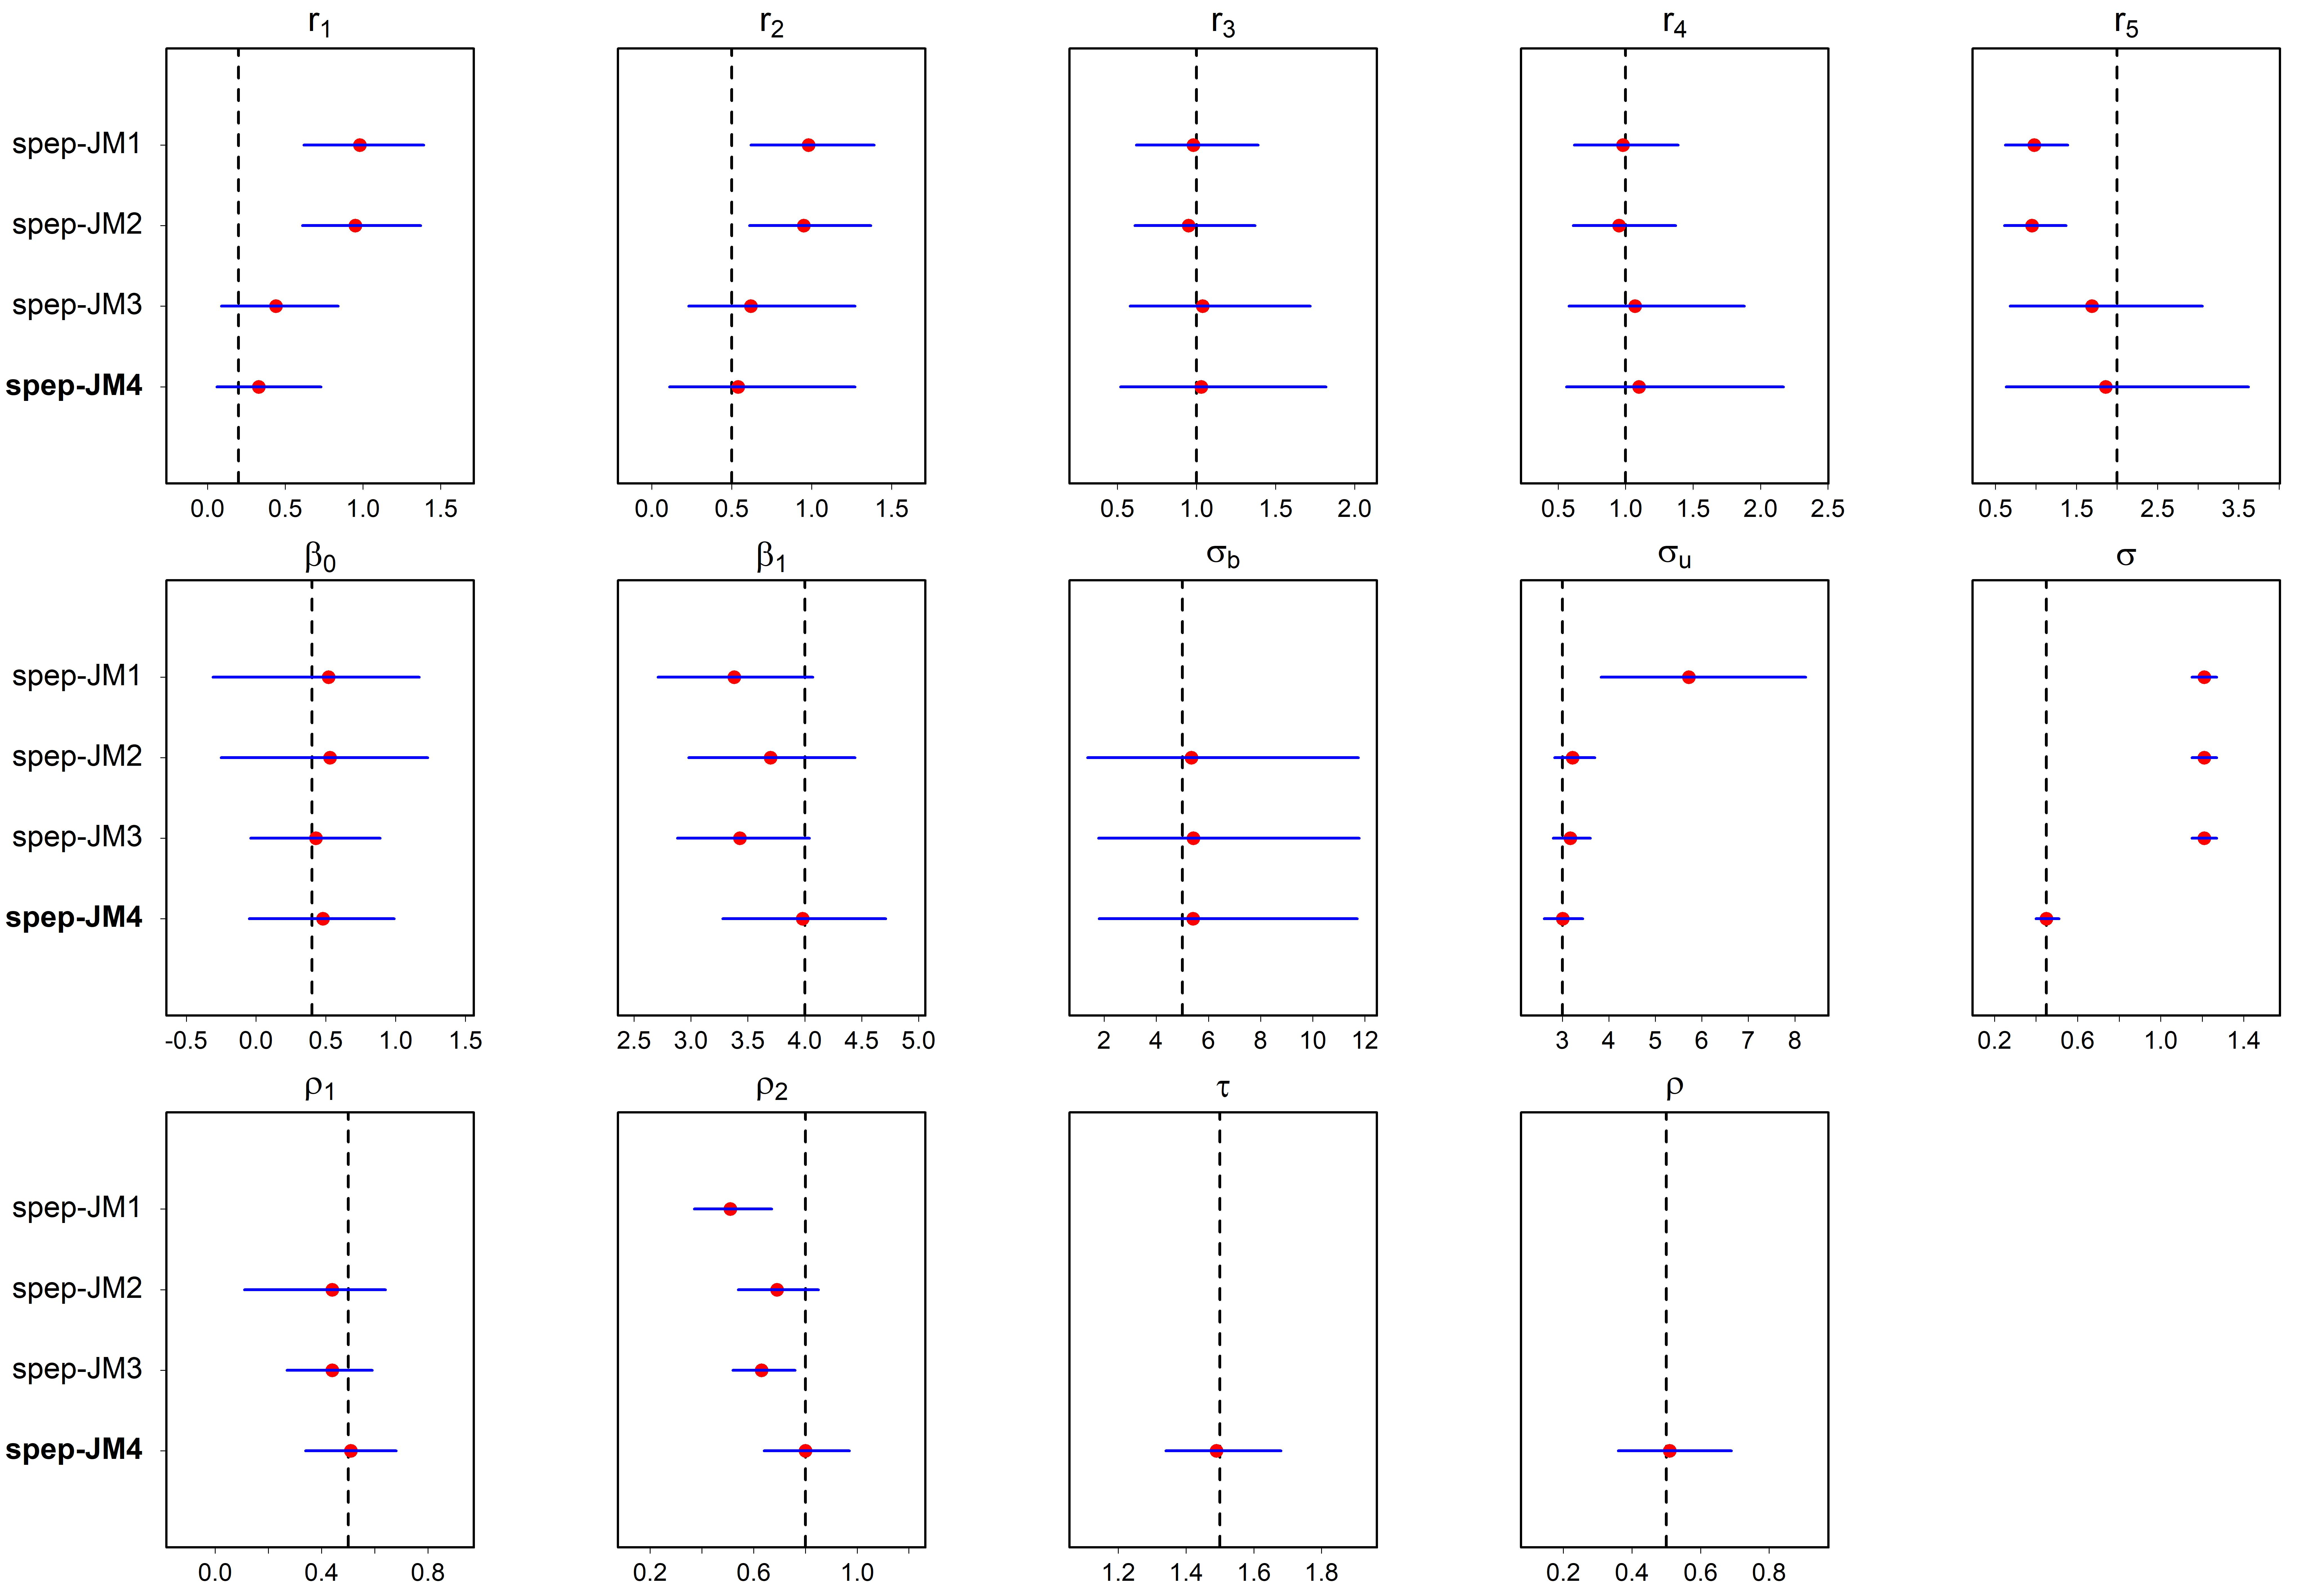
\includegraphics[width=0.8\textwidth]{Figures/Chp2_SIM_SPEP_B.jpg}
\caption{\tiny Averaged \textcolor{red}{posterior means (red dot)} with \textbf{true model (boldface)}, true value (dashed line) and \textcolor{blue}{95\% credible interval (blue line)} for 50 replicates via RStan}
\end{figure}

\note{In the plot for simulation estimates, we observe the excellent performance of proposed joint model by recovering true values. The striking biases from all other three joint models are found from scale parameter ($\sigma$) for the measurement error. In addition, we note the scale parameter $\sigma_u$ produced from non-hierarchical JM1 is kind of misleading.}

\end{frame}

\begin{frame}{Motivating Data}

\begin{columns}
        \column{0.7\textwidth}
            \begin{figure}[ht]
                \includegraphics[width=\textwidth]{Figures/Chp2_display.jpg}
            \end{figure}
        \column{.3\textwidth}
        \small
        \begin{itemize}
        \scriptsize
            \item Censor at death/lung transplant
            \item Review year 2003+
            \item Age 6-12 years
            \item Num obs. 3+ spanning 6+ months
            \item Random 5 centers
            \item 381 patients
        \end{itemize}
    \end{columns}

\note{Since the simulation study validates the capability of our proposed joint model, now we'd like to move to our motivating example. The bullets on the right panel are some key inclusive criteria that result in a total of 381 patients from 5 centers. The plot for these patients on the left panel displays the non-linear nature of ppFEV1 and some underlying skewness of PEx responses.}
\end{frame}

\begin{frame}
\frametitle{Motivating Data: WAIC}
\footnotesize
\begin{table}[H]
 \caption{\scriptsize Model comparisons for CF data with the boldface as the optimal model}
   \begin{threeparttable}
  \begin{tabular}{llll}
    \toprule
 Fitted Model & $\mbox{WAIC} \tnote{a} $ & $\mbox{WAIC}_1 \tnote{b} $ & $\mbox{WAIC}_2 \tnote{c} $ \\
 \midrule 
   Non-hierarchical (spep-$\mbox{JM}_1$) & 49960.1 &	44302.0	& 5658.1\\
   Common power (spep-$\mbox{JM}_2$) & 49867.6 &	44244.8	& 5622.8\\
   Naive LME (spep-$\mbox{JM}_3$)  & 49812.0 & 44228.0 & 5584.0\\
   \bf Proposed (spep-$\mbox{JM}_4$) & \bf 47082.3 & \bf 42704.8 & \bf 4377.5\\
    \bottomrule
  \end{tabular}
   \begin{tablenotes}[para]
    \tiny
    \item[a] Joint model; \item[b] Longitudinal continuous submodel; \item[c] Longitudinal binary submodel
    \end{tablenotes}
     \end{threeparttable}
\end{table}
\note{We fit the analysis data to four joint models which are defined previously in the simulation 2. The results of WAIC reconcile with that in the simulation study. By comparison, our proposed joint model 4 outperforms others with the lowest WAIC. And again, the non-hierarchical JM1 might induce biases for our motivating data.}
\end{frame}

\begin{frame}
\frametitle{Motivating Data: Estimates}
\setcounter{footnote}{0}
\renewcommand*{\thefootnote}{\fnsymbol{footnote}}
\begin{itemize}
    \item \textbf{Longitudinal continuous outcome: ppFEV1}
    \begin{itemize}
        \item Positive: baseline ppFEV1, BMI percentile, Genotype F508 Heter
        \item Negative: Methicillin-resistant Staphylococcus aureus (MRSA), pseudomonas aeruginosa (pa) \footnotemark[1]
    \end{itemize}
    \item \textbf{Longitudinal binary outcome: PEx}
    \begin{itemize}
        \item Negative: time, BMI percentile, pancreatic enzymes, pa
    \end{itemize}
    \item \textbf{Association Parameter}
    \begin{itemize}
        \item center\footnotemark[1] strength: $\rho_1 = -0.20 (-0.81, 0.63)$
        \item patient strength: $\rho_2 = -0.44 (-0.68, -0.3)$
    \end{itemize}
\end{itemize}
\footnotetext[1]{\tiny Not statistically significant}

\note{Here we briefly summarize predictors' positive and negative impacts for two outcomes. These predictors were selected by STEPWISE algorithm in a preliminary analysis. The negative association parameter $\rho_1,\rho_2$ is helpful to interpret that the center with more severe patients and patients with lower averaged lung function are more likely to experience PEx events.}
%We use the STEPWISE algorithm to select all following predictors from a two-stage approach. 
\end{frame}

\begin{frame}
\frametitle{Motivating Data: Performance}
\begin{table}[ht]
 \caption{\scriptsize Predictive performance between training and testing cohorts} \label{tab:chp2_pd}
  \centering
  \resizebox{\columnwidth}{!}{%
   \begin{threeparttable}
  \begin{tabular}{lrcccrccc}
    \toprule
  & \multicolumn{4}{c} {Training} &  \multicolumn{4}{c} {Testing}\\
    \cmidrule(lr) {2-5} \cmidrule(lr) {6-9}
     & \multicolumn{2}{c} {ppFEV1} &  \multicolumn{2}{c} {PEx} & \multicolumn{2}{c} {ppFEV1} &  \multicolumn{2}{c} {PEx}\\
    \cmidrule(lr) {2-3} \cmidrule(lr) {4-5} \cmidrule(lr) {6-7} \cmidrule(lr) {8-9}
 Fitted Model & RMSE & SE & AUC & 95\% CI & RMSE & SE & AUC & 95\% CI \\
 \midrule
   
   {Non-hierarchical (spep-$\mbox{JM}_1$)}
  & 10.755 & 0.142 & 0.748 & (0.734, 0.763) & 10.397 & 0.233 & 0.623 & (0.594, 0.651)\\

   {Common power (spep-$\mbox{JM}_2$)}
  & 10.686 & 0.141 & 0.748 & (0.734, 0.763)	& 10.399 & 0.233 & 0.622 & (0.593, 0.651)\\

   {Naive LME (spep-$\mbox{JM}_3$)}
  & 10.671 & 0.141 & 0.755 & (0.741, 0.770) & 10.398 & 0.233 & 0.639 & (0.610, 0.667)\\
   {\bf Proposed (spep-$\mbox{JM}_4$)}
   & \bf 7.768	& \bf 0.102 & \bf 0.882 & \bf (0.873, 0.892) & \bf 6.879 & \bf 0.154 & \bf 0.631 & \bf (0.604, 0.658)\\
    \bottomrule
  \end{tabular}
   \begin{tablenotes}[para]
    \footnotesize
    Model in boldface: optimal model; Abbreviations: RMSE=Root Mean Square Error; SE=Standard Error; AUC=Area under Curve; CI=Confidence Interval 
    \end{tablenotes}
    \end{threeparttable}%
}
\end {table}

\note{To access the predictive performance, we evaluate RMSE for ppFEV1 and AUC for PEx. As RMSE is an error term, thus the smaller value the better, but for AUC, the higher AUC indicates the better of model at distinguishing between PEx and non-PEx events. As shown in the table, our optimal model achieves reasonable accuracy for new patients compared to all other three joint models.}
\end{frame}


\begin{frame}
\frametitle{Motivating Data: Performance (cont'd)}
\begin{table}[ht]
\caption{\scriptsize Forecasting performance between training and masking cohorts} \label{tab:chp2_fc}
\centering
\resizebox{\columnwidth}{!}{%
 \begin{threeparttable}
  \begin{tabular}{lrcccrccc}
    \toprule
  & \multicolumn{4}{c} {Training} &  \multicolumn{4}{c} {Masking}\\
    \cmidrule(lr) {2-5} \cmidrule(lr) {6-9}
     & \multicolumn{2}{c} {ppFEV1} &  \multicolumn{2}{c} {PEx} & \multicolumn{2}{c} {ppFEV1} &  \multicolumn{2}{c} {PEx}\\
    \cmidrule(lr) {2-3} \cmidrule(lr) {4-5} \cmidrule(lr) {6-7} \cmidrule(lr) {8-9}
 Fitted Model & RMSE & SE & AUC & 95\% CI & RMSE & SE & AUC & 95\% CI \\
 \midrule
   
   {Non-hierarchical (spep-$\mbox{JM}_1$)}
  & 10.755 & 0.142 & 0.748 & (0.734, 0.763) & 10.354 & 0.272 & 0.655 & (0.626, 0.683) \\

   {Common power (spep-$\mbox{JM}_2$)}
  & 10.686 & 0.141 & 0.748 & (0.734, 0.763)	& 10.298 & 0.270 & 0.628 & (0.598, 0.658)\\

   {Naive LME (spep-$\mbox{JM}_3$)}
  & 10.671 & 0.141 & 0.755 & (0.741, 0.770) & 10.353 & 0.271 & 0.612 & (0.582, 0.642)\\
   {\bf Proposed (spep-$\mbox{JM}_4$)}
   & \bf 7.768	& \bf 0.102 & \bf 0.882 & \bf (0.873, 0.892) & \bf 8.850 & \bf 0.233 & \bf 0.785 & \bf (0.760, 0.809)\\
    \bottomrule
  \end{tabular}
    \begin{tablenotes}[para]
    \footnotesize
     Model in boldface: optimal model; Abbreviations: RMSE=Root Mean Square Error; SE=Standard Error; AUC=Area under Curve; CI=Confidence Interval 
    \end{tablenotes}
    \end{threeparttable}%
    }
 \end {table}
\note{With respect to the existing patients, again our optimal joint model 4 is superior to others with excellent predictive performance}
\end{frame}

\begin{frame}
\frametitle{Motivating Data: Prediction}
\begin{figure}[ht]
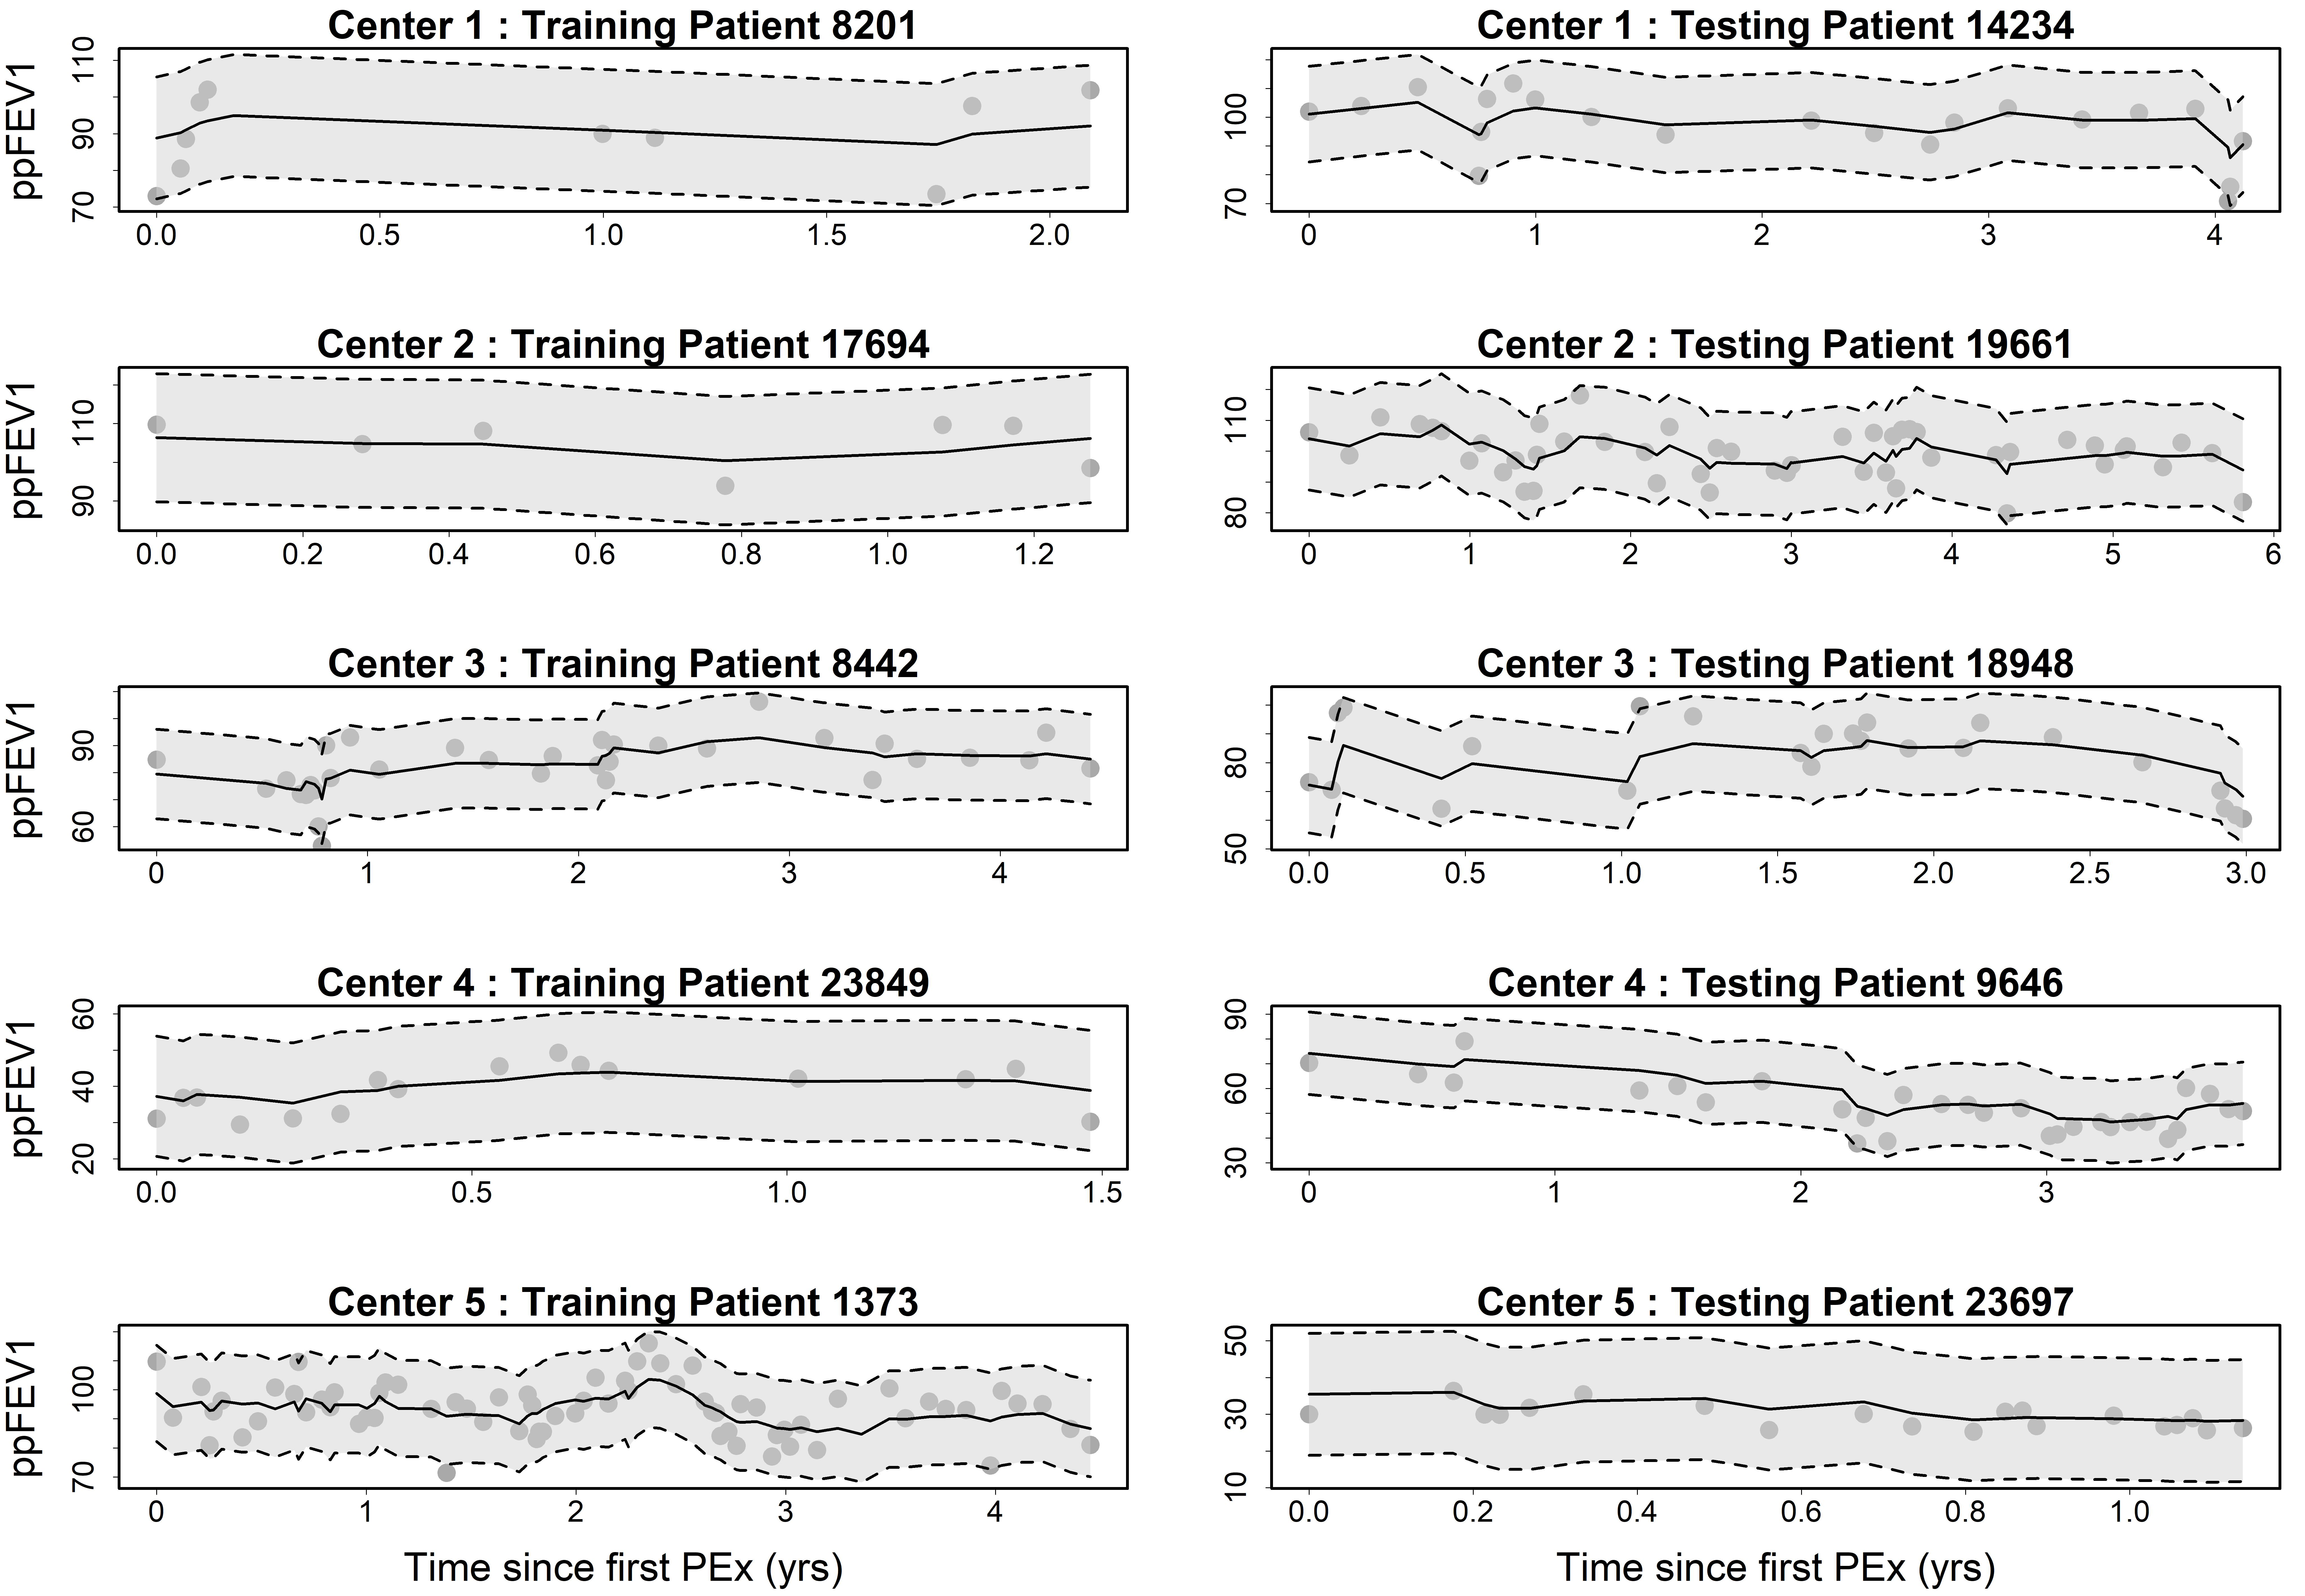
\includegraphics[width=0.9\textwidth]{Figures/Chp2_pred.jpg}
\end{figure}
\note{We plot predictions of ppFEV1 for some random patients, gray dots are observed values, black lines with bands are fitted values with 95\% confidence intervals. Our optimal joint model by accounting for Gaussian process is well shown to capture the heterogeneous trajectory of ppFEV1}
\end{frame}

\begin{frame}
\frametitle{Motivating Data: Forecast}
\begin{figure}[ht]
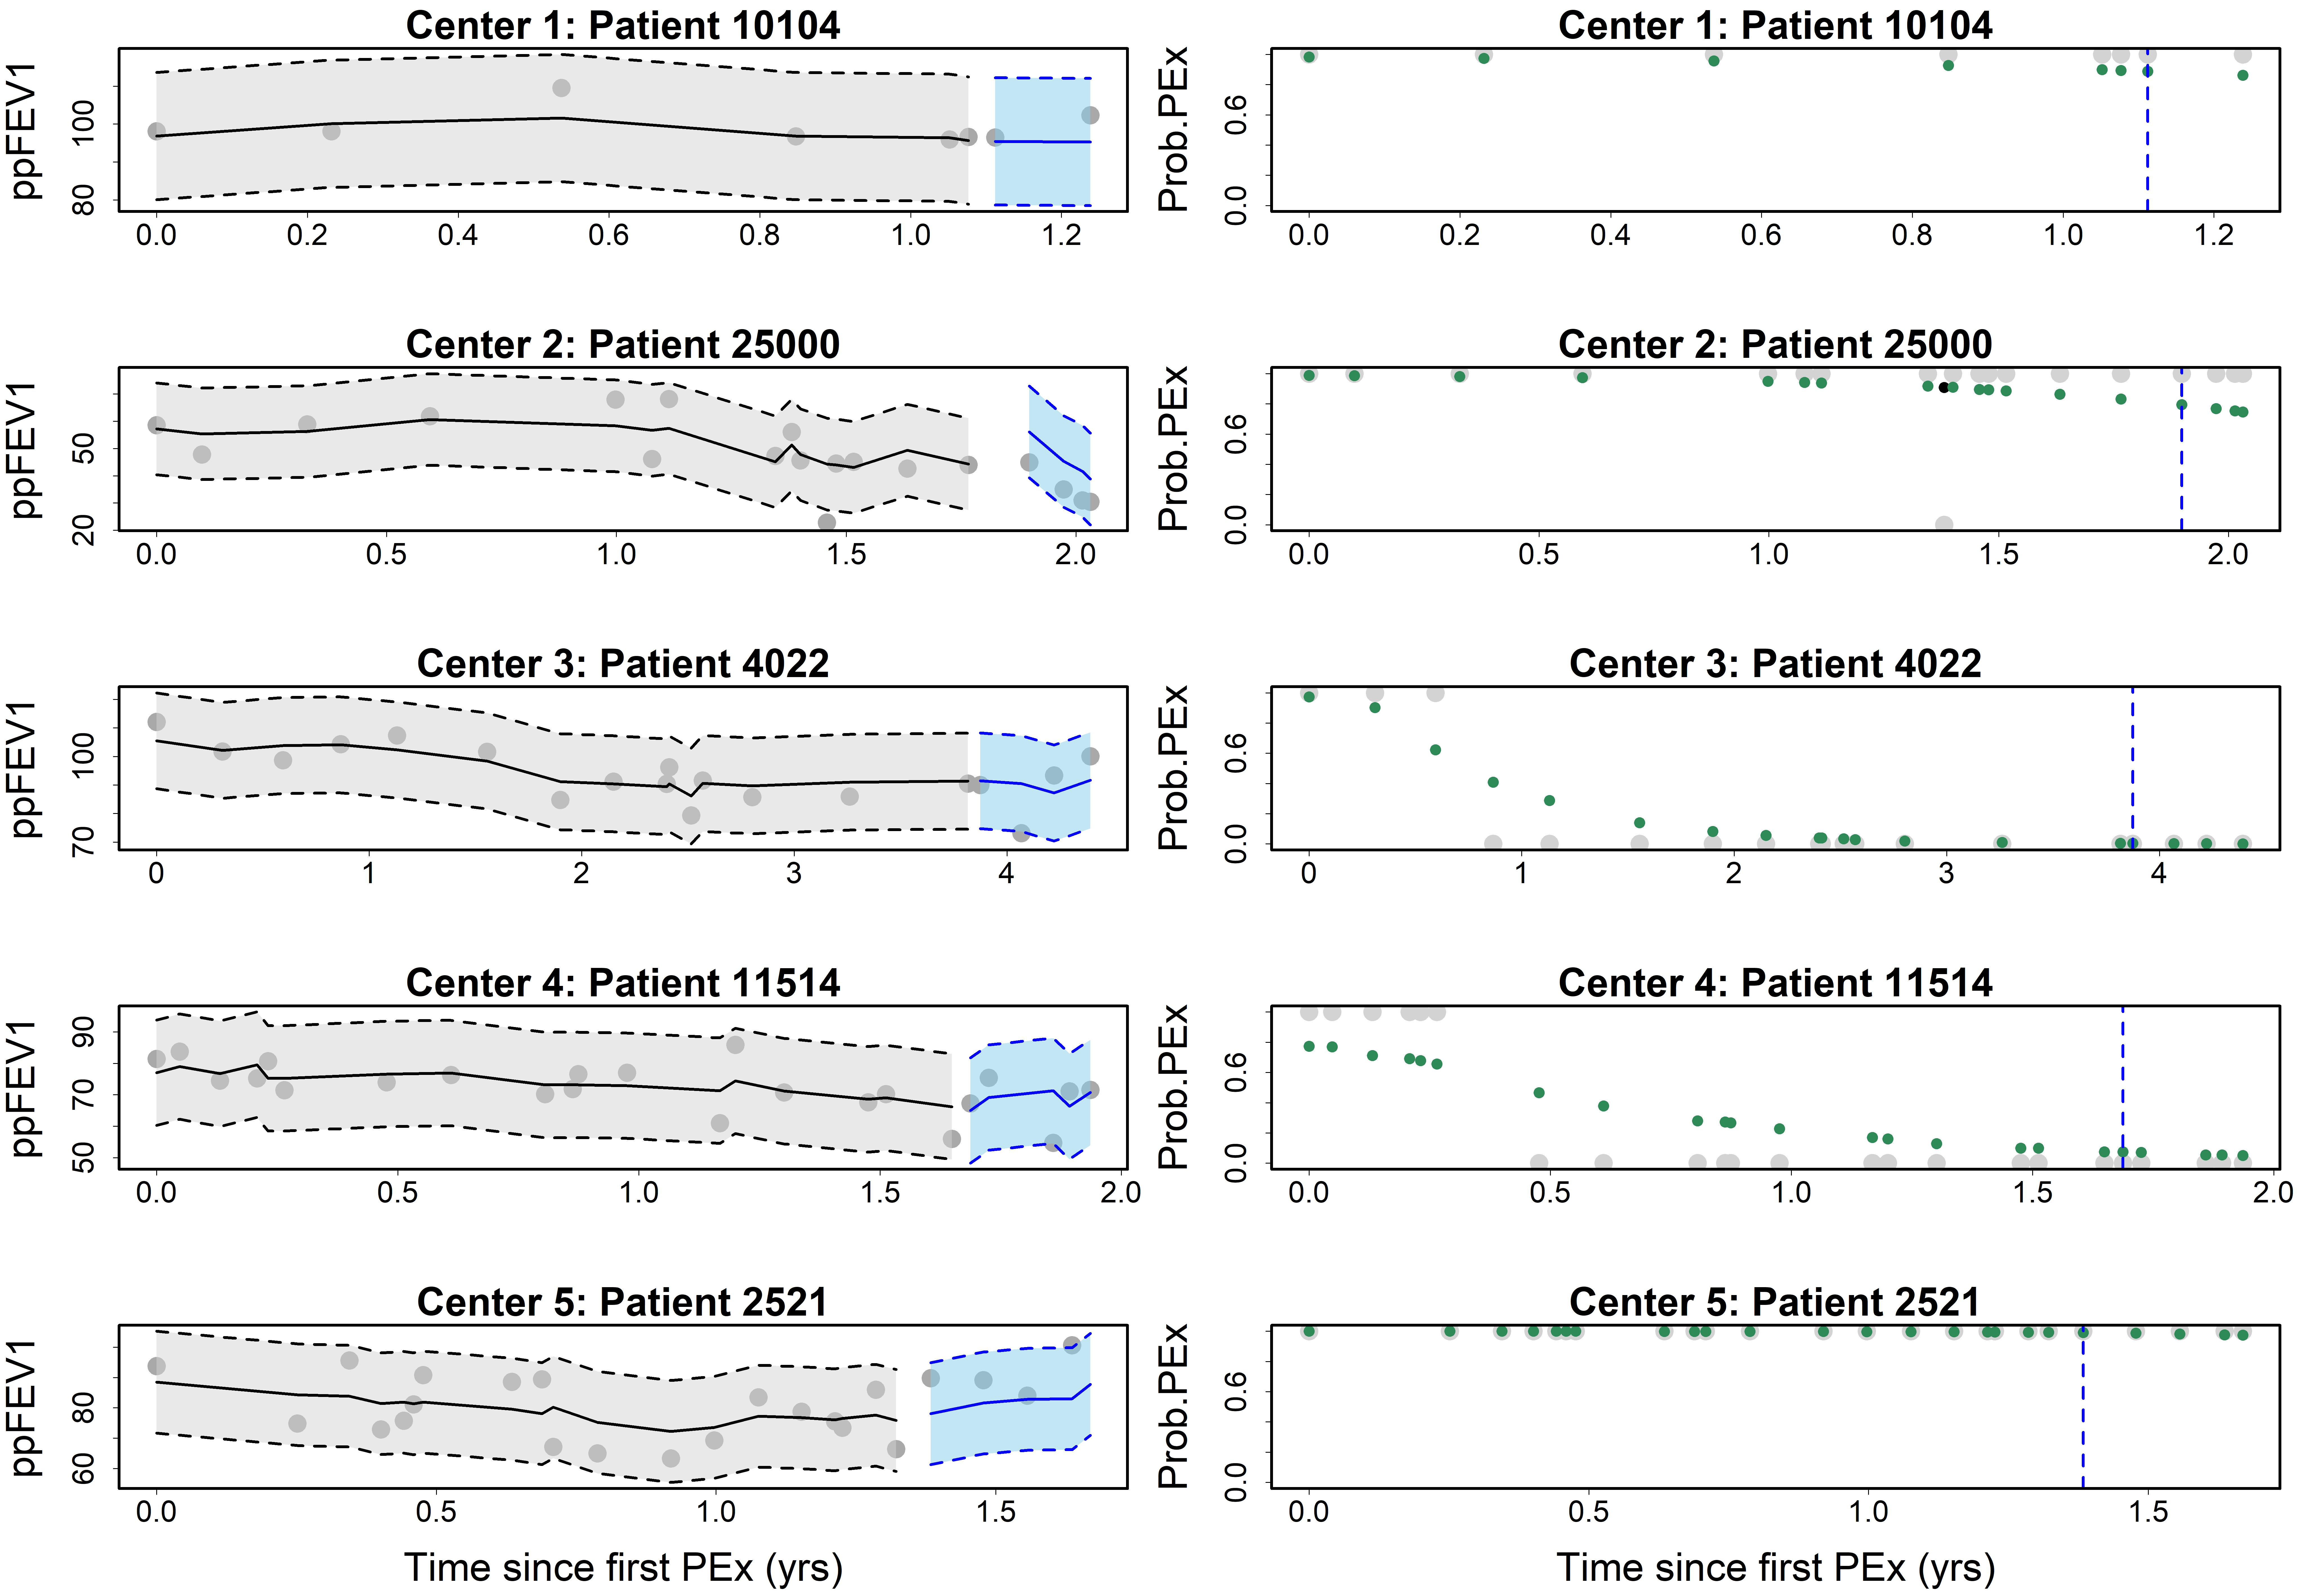
\includegraphics[width=0.9\textwidth]{Figures/Chp2_mask.jpg}
\end{figure}
\note{For existing patients, we plot dynamic forecast period in blue and predictive probability of PEx events, with green dots for the true identification. Again, our optimal joint model shows reasonable predictive accuracy. }
\end{frame}

\begin{frame}
\frametitle{Discussion}
\setcounter{footnote}{6}
\begin{itemize}
    \item \textbf{Features}
    \begin{itemize}
        \item Stochastic Gaussian process 
        \item Flexible link with center-specific power parameter
        \item Dynamic individual prediction
        \item Non-hierarchical joint model biases
    \end{itemize}
    \item \textbf{Extensions}
    \begin{itemize}
        \item Predict new patients from a new center
        \item Flexible link family based on GEV\footnotemark distribution {\scriptsize(\cite{Wang2010})}
        \item Time-dependent association structure (e.g., latent Gaussian process)
    \end{itemize}
\end{itemize}
\footnotetext[6]{\tiny Generalized Extreme Value}
\note{To conclude for this project, we proposed a multilevel joint model that incorporates stochastic Gaussian process and a flexible link function to facilitate the dynamic individual prediction. In parallel, we explore the biases caused from the non-hierarchical joint model. Also there are some interesting extensions: i) we can further generalize the individual prediction method to account for a new patient from a new center; ii) or we can apply an alternative flexible link function based on GEV distribution; iii) or we can extend the association structure to be time-dependent to improve the model performance. }
\end{frame}


\section[Project II: Recurrent Outcome]{Multilevel Bayesian Joint Model of Longitudinal and Recurrent Outcomes}
\setcounter{subsection}{1}

\begin{frame}
\frametitle{}
% \begin{center}
% \textbf{\Large Multilevel Bayesian Joint Model of Longitudinal and Recurrent Outcomes}
% \end{center}
\begin{enumerate}
    \item<0> \textbf{Introduction}
    \item<0> \textbf{Multilevel Bayesian Joint Model of Longitudinal and Binary Outcomes}
    \begin{itemize}
        \item Motivation
        \item Model framework
        \item Simulation study \& Motivating data
        \item Discussion
    \end{itemize}
    \item \textbf{Multilevel Bayesian Joint Model of Longitudinal and Recurrent Outcomes}
    \begin{itemize}
        \item Motivation
        \item Model framework
        \item Simulation study \& Motivating data
        \item Discussion
    \end{itemize}
    \item<0> \textbf{Conclusion and Future Work}
\end{enumerate}
\note{Recall that in the previous project, we regard PEx as the longitudinal binary outcome. It might be also of clinical interest to predict the time-to-recurrent event, which means to treat PEx in a survival context. So in my project 2, I will introduce you a multilevel Bayesian joint model of longitudinal and recurrent outcomes}
\end{frame}


\begin{frame}
\frametitle{Motivation}
\begin{itemize}

    \item Time-to-recurrent PEx in two risk scales
    \item Center-specific time-dependent association structure
    \item Prognostic utility of the optimal joint model
    
\end{itemize}

\note{Our motivation is threefold: i) Study repeated PEx in two risk scales; ii) We want to investigate a center-specific time-dependent association structure; iii) Evaluate the predictive performance of the optimal joint model 
}
\end{frame}


\begin{frame}
\frametitle{Risk Scales}
\begin{columns}
\column{.7\textwidth}
\begin{figure}[ht]
\centering
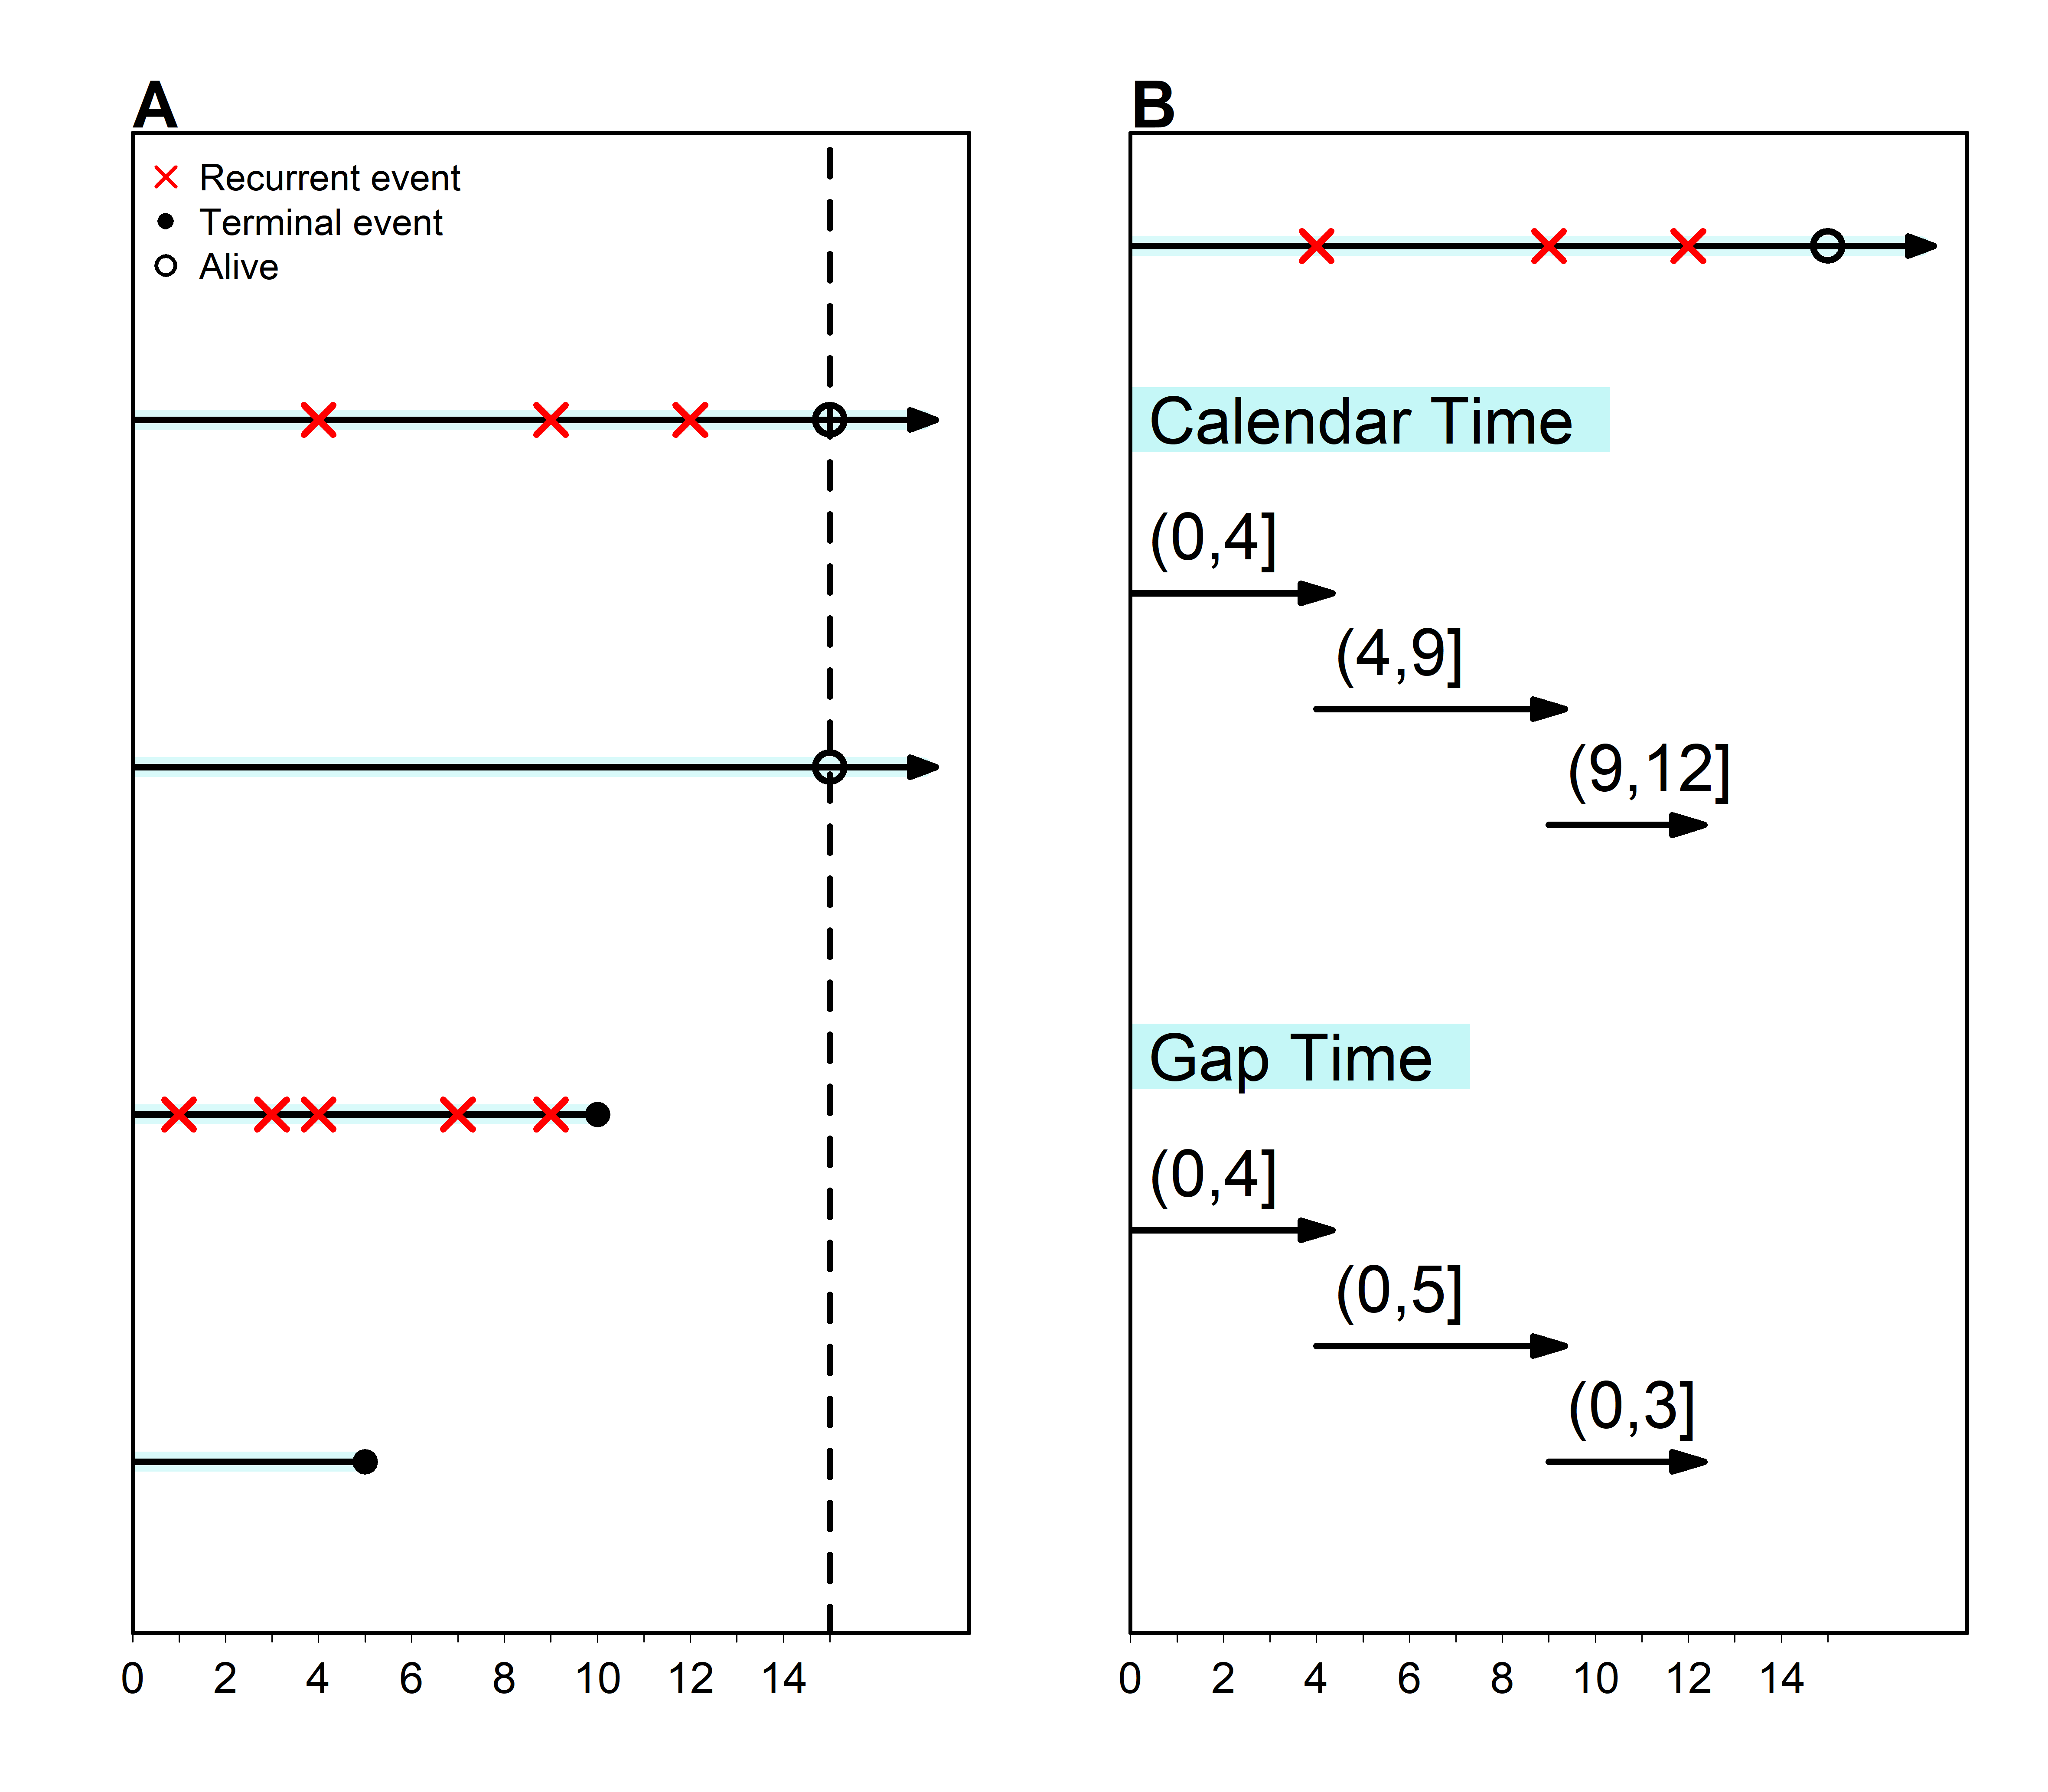
\includegraphics[width=0.9\textwidth]{Figures/Chp3_censor.png}
\end{figure}
\column{.5\textwidth}

\begin{itemize}
    \item \textbf{calendar time} 
    \begin{itemize}
        \item \scriptsize effect from \textcolor{red}{entry time}
    \end{itemize}
    \item \textbf{gap time}: 
    \begin{itemize}
        \item \scriptsize effect from previous \textcolor{red}{end time}
    \end{itemize}
\end{itemize}
\end{columns}
\note{The Figure A displays four possible patients who are censored either at a terminal event or the end of observed time. If we zoom in to the patient with repeated events, we can estimate the effect through two risk scales: Calendar and gap time as shown in Figure B. They are of the same interval time length, however, interpretations for them are different. Specifically, calendar time evaluates the effect of a covariate from the entry time, while gap time evaluates the effect of a covariate from the end time of the previous event. 
% There is a third type of time scale, known as total time. Because it is unrealistic for the individual prediction, thus I am not interested in it
}
\end{frame}

\begin{frame}
\frametitle{Model Framework}

\footnotesize {Let $l,i,j$ be as before; $k \in j$ denote recurrent time point.}

\begin{itemize}
    \item \textbf{Longitudinal submodel}:
    \begin{align}
    \mbox{LME}  \left \{\begin{array}{ll}
    y_{lij}(t)=m_{lij}(t)+\epsilon_{lij}(t)\\
    m_{lij}(t)=\bm{x}^T_{lij}(t)\bm{\beta}+b_l+\bm{z}^{T}_{lij}(t)\bm{U}_{li}
    \end{array}\right.
\end{align}
where $b_l \sim N(0,\sigma_b), \bm{U}_{li} \sim N(\bm{0},\Sigma_u), \epsilon_{lij} \sim N(0, \sigma)$, $\bm{b} \ind \bm{U} \ind \bm{\epsilon}$. 

    \item \textbf{Recurrent event submodel}: 
    \begin{align}
    \mbox{ESRRFM} \footnotemark \left \{\begin{array}{ll}
        h_{lik}(t)=h_{l0}(t)exp\big\{\bm{\omega}^T_{lik}(t)\bm{\gamma}+f(\bm{\beta},b_l,\bm{U}_{li},\alpha_l;t)+v_{li}\big\} \\
        h_{l0}(t)=\delta_l t^{\delta_l-1} (Weibull)
      \end{array}\right.
    \end{align}
where $\delta_l \in (0, +\infty), v_{li} \sim N(0,\sigma_v)$, $f(\cdot)$ denotes time-dependent association structure. 
\end{itemize}
\footnotetext[7]{\tiny Extended Stratified Relative Risk Frailty Model}
\note{For the model framework, we have the same index as before with an additional time point index k for recurrent events. Again, we adapt to a shared parameter joint model. For the longitudinal submodel, we still set up an LME, having function $m$ as the linear predictor of ppFEV1, but this time we have random intercept b for center and random intercept and slope U for patient without Gaussian process. In the event submodel, we implement an extended stratified relative risk model with frailty term. The stratification is subject to center-specific baseline hazard function, with an assumption of the Weibull distribution. $\bm{\omega}$ is a vector of individual covariates (possibly time-dependent) with corresponding regression coefficient $\bm{\gamma}$ (also known as log hazard ratio).$f(\cdot)$ denotes the time-dependent association structure, which will be discussed in the next slide. $v$ is a random effect that accounts for the correlation between repeated events. The $exp(v)$ is also well known as the frailty term in the survival analysis.}

\end{frame}


\begin{frame}{Association Structure}

linear predictor of ppFEV1:  $m_{lik}(t)=\bm{x}^T_{lik}(t)\bm{\beta}+b_l+\bm{z}^{T}_{lik}(t)\bm{U}_{li}$

\begin{align}
     \left \{\begin{array}{ll}
        \mbox{Current value: }f(\bm{\beta}, b_l, \bm{U}_{li}, \alpha_{v_l}; t)=\alpha_{v_l} \times m_{lik}(t)\\\\
        \mbox{Current slope: }f(\bm{\beta}, b_l, \bm{U}_{li}, \alpha_{s_l}; t)=\alpha_{s_l} \times \displaystyle \frac{d}{dt} m_{lik}(t)   
        \end{array}\right.
    \end{align}

\note{The association structure can be parameterized in many ways, here we only consider current value and current slope of the linear predictor from preliminary analysis, they are expressed in Equation 13. To account for hierarchical data structure, we assign the center-specific association parameter to each of them.}

\end{frame}


\begin{frame}
\frametitle{Bayesian Inference}

\begin{itemize}
    \item Joint posterior distribution is given by
    \scriptsize
    \begin{align}
        p(\bm{\theta},b_l,\bm{U}_{li},v_{li}|\bm{y}_{li}, \bm{t}_{li}, \bm{d}_{li}) \propto & \prod_jp(y_{lij}|b_l,\bm{U}_{li},\bm{\theta})
        \times \prod_kp(t_{lik},d_{lik}|b_l,\bm{U}_{li},v_{li},\bm{\theta})\\\nonumber 
        & \times p(b_l|\bm{\theta})p(\bm{U}_{li}|\bm{\theta})p(v_{li}|\bm{\theta})p(\bm{\theta})
    \end{align}
where $t_{lik}$ is the observed event time and $d_{lik}$ is the event indicator.

    \item Log likelihood for event submodel
    
    \begin{itemize}
    \scriptsize
        \item Calendar time
        \begin{align}
       \mbox{log } p(t_{lik}, d_{lik}|b_l,\bm{U}_{li},v_{li},\bm{\theta}) = d_{lik} \cdot \mbox{log } h_{li}(t_{lik}) - \int^{t_{lik}}_{t_{li(k-1)}} h_{li}(s)ds 
    \end{align}
    
        \item Gap time
        \begin{align}
        \mbox{log } p(t_{lik}, d_{lik}|b_l,\bm{U}_{li},v_{li},\bm{\theta}) = d_{lik} \cdot \mbox{log } h_{li}(t_{lik}-t_{li(k-1)}) - \int^{t_{lik}-t_{li(k-1)}}_{0} h_{li}(s)ds
    \end{align}
    \item Gauss-Kronrod (GK) quadrature with Q nodes {\scriptsize (\cite{Laurie1997})}
    \end{itemize}
    
\end{itemize}
\note{Recall the assumption of conditional independence, by which the joint posterior distribution can be derived from Equation 14. The likelihood for longitudinal submodel is straightforward, so not present here, while the log likelihood function for the event submodel under two risk scales can be specified by Equation 15 \& 16. The latter integral term can be approximated by Gauss-Kronrod(GK) quadrature with Q nodes. Furthermore, we assume our data is non-informative right censoring.}
\end{frame}

\begin{frame}
\frametitle{Computation}
\footnotesize
\begin{table}[H]
\begin{threeparttable}
 \begin{tabular}{lcc}
    \toprule
 HMC & Simulation Study & Motivating Data \\
 \midrule 
 Interface to Stan & cmdstanr & cmdstanr \\
 Post-warmup\tnote{+} & 2000 & 2000 \\
 Chains & 2 & 2\\
    \bottomrule
  \end{tabular}
  \begin{tablenotes}
  \item[\textsuperscript{+}] \tiny Converged samplings validated by $\widehat{R}$ (\cite{Gelman1992})
  \end{tablenotes}
\end{threeparttable}
\end{table}
\note{The posterior samplings are carried out through HMC by the interface cmdstanr}
\end{frame}


\begin{frame}
\frametitle{Prior Distributions}
\scriptsize
$$\beta_0 \sim N(0,100),$$
$$\beta_p \sim N(0,\phi_\beta), p=1,2,\dots,P-1,$$
$$\sigma \sim \mbox{Truncated } N(0,\phi_\sigma),$$
$$\sigma_b \sim \mbox{Truncated } N(0,10),$$
$$\sigma_{u0}, \sigma_{u1} \sim \mbox{Truncated } t(1,0,10),$$
$$
\begin{bmatrix}
1 & \rho \\
\rho & 1
\end{bmatrix}  \sim lkjCorr(2), $$
$$\gamma_0 \sim N(0,20),$$
$$\gamma_q \sim N(0,\phi_\gamma), q=1,2,\dots, Q-1,$$
$$\lambda_l \sim \mbox{Truncated } N(0,5), l=1,2,\dots,L,$$
$$\sigma_v \sim \mbox{Truncated } N(0,10)$$

where $\phi_\beta,\phi_\gamma$ are sds of corresponding design matrix, $\phi_\sigma$ is sd of longitudinal outcomes. \\
\tiny
Note: sd=standard deviation; Normal(location,scale); student-t(df,location,scale); LKJ correlation(shape). 

\note{We assign mutually independent diffuse or weakly informative priors for all unknown parameters.
% Unlike previous project, we have set up Normal distribution for most of the priors. 
lkjCorr denotes LKJ correlation matrix density, is particularly constructed for the correlation matrix.}

\end{frame}


\begin{frame}
\frametitle{Individual Prediction}

\begin{itemize}
    \item \small \textbf{ppFEV1}
      \scriptsize
    \begin{align} \label{eq:indpred}    
    p(\tilde{y}_{lij}(t)|\mathcal{D}) & =\int\int\int p(\tilde{y}_{lij}(t)|b_l,\bm{U}_{li},\bm{\theta}) p(b_l,\bm{U}_{li},\bm{\theta}|\mathcal{D}) \,  db_l \,  d\bm{U}_{li} \, d\bm{\theta} \\\nonumber
     & \approx \frac{1}{M} \sum_{m=1}^{M} p(\tilde{y}_{lij}(t)|b_l^{(m)},\bm{U}_{li}^{(m)},\bm{\theta}^{(m)},\mathcal{D})
\end{align}
    \item \small \textbf{probability of next PEx-free event}
     \scriptsize
    \begin{align} \label{eq:cond.surv}
        S_{li}(t'|t) & = p(t_{n^*_{li}+1} \geq t'|t_{n^*_{li}+1} > t, \mathcal{D})  \\\nonumber
                    & = \int\int\int\int p(t_{n^*_{li}+1} \geq t'|t_{n^*_{li}+1} > t, b_l,\bm{U}_{li},v_{li},\bm{\theta},\mathcal{D}) \\\nonumber
                    & \cdot p(b_l, \bm{U}_{li}, v_{li}, \bm{\theta} |t_{n^*_{li}+1} > t, \mathcal{D}) \, db_l \, d\bm{U}_{li} \, dv_{li} \, d\bm{\theta} \\\nonumber
        & \approx \frac{1}{M} \sum_{m=1}^{M} exp\Big[ -\int_t^{t'} h\big(s|b_l^{(m)},\bm{U}_{li}^{(m)},v_{li}^{(m)},\bm{\theta}^{(m)}\big) ds \Big]
\end{align}
where $\mathcal{D}$ is observed data, $n^*_{li}(n^*_{li}=0,1,2,\dots)$ denotes recurrent events up to the time $t$ and $t' > t$. 

\end{itemize}
\note{Now we come to the method of individual prediction for in-sample patients. The expected value for ppFEV1 at time $t$, can be generated from the posterior predictive distribution as shown in Equation 17. Through the Monte Carlo method, we can approximate it by drawing samplers from the posterior distribution. For event-free probability, we derive the conditional survival probability between time frame t and t' in Equation 18. Again we can approximate integrals by Monte Carlo method and the integral term from survival function can be evaluated by GK quadrature again.}
\end{frame}


\begin{frame}
\frametitle{Predictive Performance}
\begin{itemize}
    
    \item Discrimination
    \begin{itemize}
        \item Time-dependent \underline{a}rea \underline{u}nder receiver operating characteristic \underline{c}urve (AUC)
    \end{itemize}
    \vspace{5mm}
    \item Calibration
    \begin{itemize}
        \item Time-dependent \underline{m}ean \underline{p}redictive \underline{e}rror (MPE) on squared loss function
    \end{itemize}
\end{itemize}
\note{To assess the predictive performance, we employ AUC for discrimination, which means to discriminate between patients who will experience the next event from patients who will not. We utilize mean predictive error for calibration, that is how well the model predicts the observed event probability. Due to the censoring property, we compute time-dependent AUC and MPE manually.}
\end{frame}

\begin{frame}

\frametitle{Leave-one-out (loo) Cross-validation}

\begin{itemize}
\footnotesize
 \item Pareto-smoothed importance sampling (PSIS) {\scriptsize (\cite{Vehtari2017})} of expected log pointwise predictive density (elpd) 
\begin{align}
 \widehat{\mbox{elpd}}_{\mbox{psis-loo}}=\sum_{l=1}^{L}\sum_{i=1}^{n_l}log\Big(\frac{\sum_{s=1}^S w^s_{li}p(y_{li}|\theta^s)}{\sum_{s=1}^S w^s_{li}} \Big)
 \end{align}

 \item LOOIC
    \begin{align}
        \mbox{LOOIC}=-2 \times \widehat{\mbox{elpd}}_{\mbox{psis-loo}}
    \end{align}
 \item Computed by loo::loo()
 \item The smaller the better
    
\end{itemize}

\note{In this project we adapt to a recent popular measure of predictive accuracy, called loo. We define LOOIC so as to be on the deviance scale. Similar to WAIC, we can get computed value by the function called loo and the model with smaller LOOIC indicates the better goodness of fit.}

\end{frame}

\begin{frame}
\frametitle{Simulation Study}

Validate Bayesian inference and compare with two-stage approach

\footnotesize
\begin{table}[H]
    \caption{\scriptsize Simulation illustration}
    %  \vspace{-5mm}
        \begin{threeparttable}
            \begin{tabular}{l|c|c}
            \toprule
        \bf Association + Risk scale & \bf True Model & \bf Fitted Model \\ \hline
        
        \multirow{2}{*}{Slope + Gap} & \multirow{2}{*}{JM1} & JM1 \\ 
        && TM1 \\\hline                           
        \multirow{2}{*}{Slope + Calendar} & \multirow{2}{*}{JM2} & JM2 \\ 
        && TM2\\
            \bottomrule
    \end{tabular}
    \begin{tablenotes}[para]
    \scriptsize
    Note:JM=Joint Model; TM=Two-stage Model
    \end{tablenotes}
    \end{threeparttable}
    \end{table}

\note{So far, we have went through model framework, including Bayesian inference, individual prediction and model selection. Now, we move forward to our simulation study. We aim to validate our Bayesian inference and meanwhile, to compare the true joint model with the corresponding two-stage model. As shown in the table, we simulate the multicenter data through true model and fit it to two models under each scenario for 50 replicates. JM stands for joint model and TM stands for Two-stage model. }
\end{frame}

\begin{frame}{Association Structure: Current Slope}
\begin{figure}[ht] 
        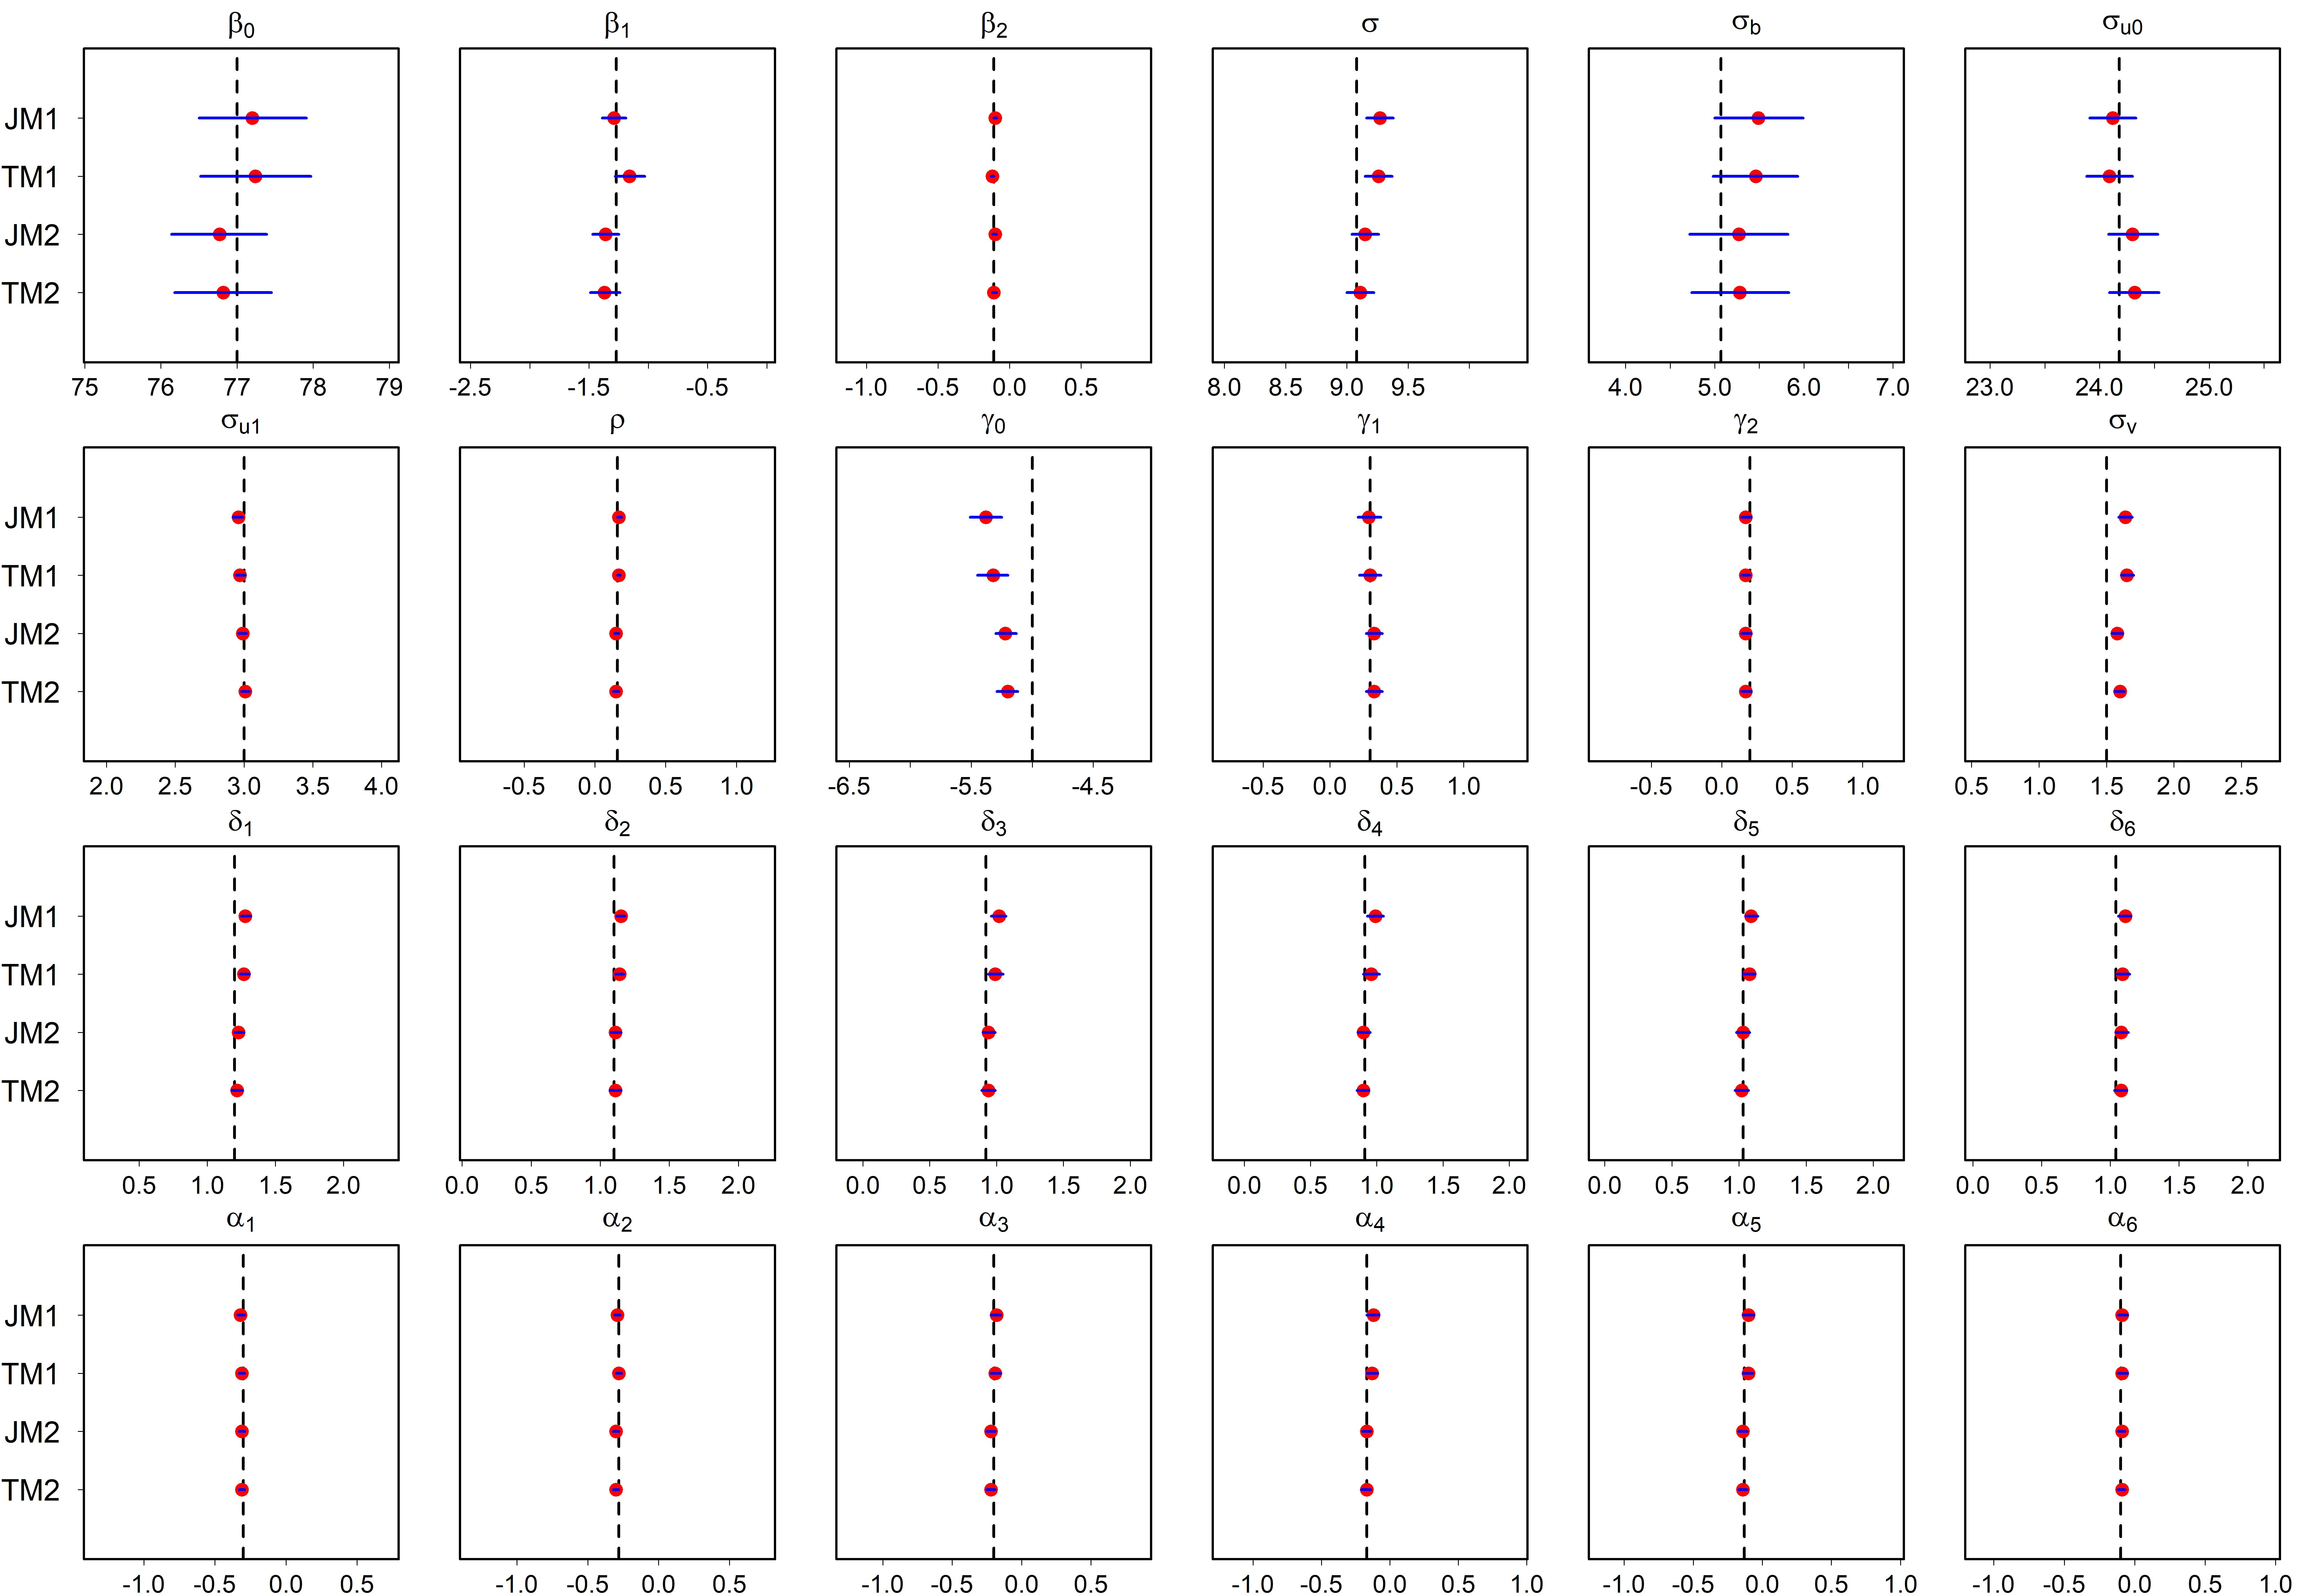
\includegraphics[width=0.8\textwidth]{Figures/Chp3_sim_1.jpg} 
        \caption{\tiny Averaged \textcolor{red}{posterior mean (red dot)} with true value (dashed line) and \textcolor{blue}{95\% confidence interval (blue line)} for 50 replicates via CmdStanr. JM1/TM1: Slope+Gap; JM2/TM2: Slope+Calendar.}
    \end{figure}

\note{We plot simulation results and expect red dot to be close to the dashed line for proposed true joint models. We note that joint models represent excellent performance in recovering the true values, which validate the Bayesian inference. And, two-stage models show very slight biases}
\end{frame}

\begin{frame}
\frametitle{Simulation Study (cont'd)}
\footnotesize
\begin{table}[H]
    \caption{\scriptsize Simulation illustration}
        \begin{threeparttable}
            \begin{tabular}{l|c|c}
            \toprule
        \bf Association + Risk scale & \bf True Model & \bf Fitted Model \\ \hline
        \multirow{2}{*}{Value + Gap} & \multirow{2}{*}{JM3} & JM3 \\ 
        && TM3\\\hline 
        \multirow{2}{*}{Value + Calendar} & \multirow{2}{*}{JM4} & JM4 \\ 
        && TM4\\
     \bottomrule
    \end{tabular}
    \begin{tablenotes}[para]
    \scriptsize
    Note:JM=Joint Model; TM=Two-stage Model
    \end{tablenotes}
    \end{threeparttable}
    \end{table}
\note{We repeat the simulation process for association structure with current value.}
\end{frame}

\begin{frame}{Association Structure: Current Value}
    \begin{figure}[ht] 
        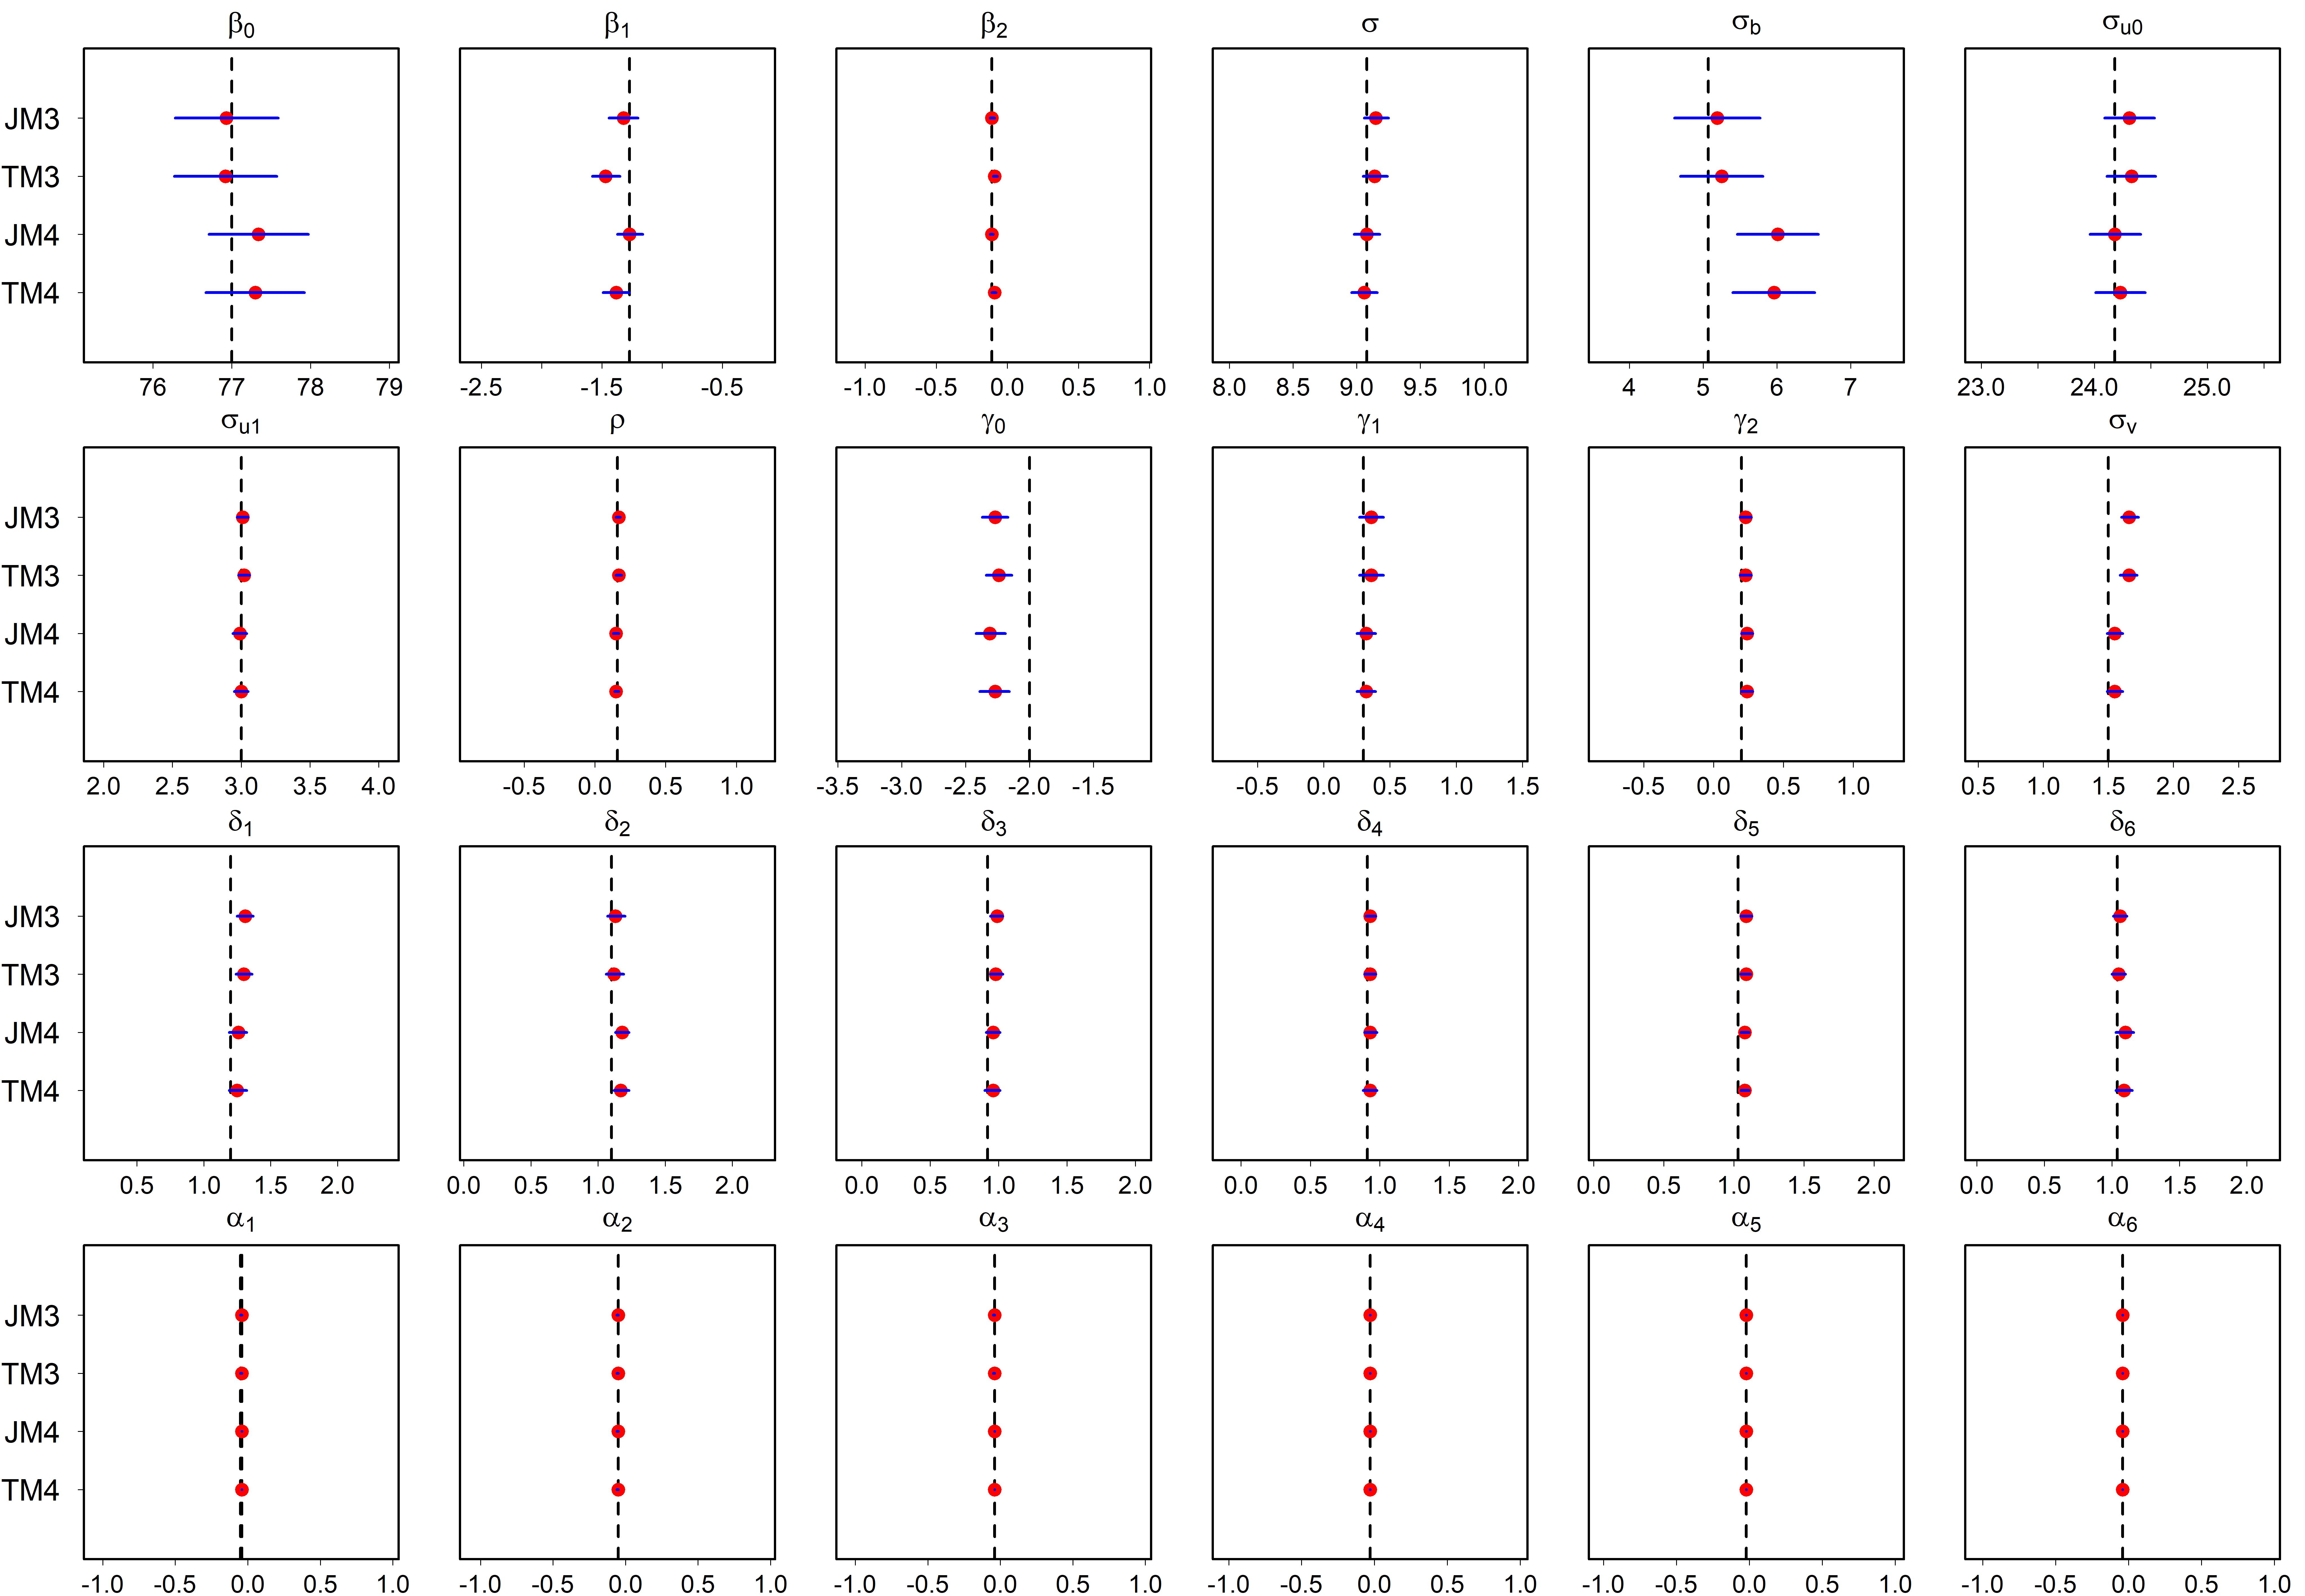
\includegraphics[width=0.8\textwidth]{Figures/Chp3_sim_2.jpg} 
        \caption{\tiny Averaged \textcolor{red}{posterior mean (red dot)} with true value (dashed line) and \textcolor{blue}{95\% confidence interval (blue line)} for 50 replicates via CmdStanr. JM3/TM3: Value+Gap; JM4/TM4: Value+Calendar.}
    \end{figure}
\note{For parameter $\beta_1$, two-stage models show some biases compared to the corresponding joint models. Other than that, both joint model and two-stage model represent similar and reasonable performance. But later on, we will tell the preference from LOOIC from the real data example.}
\end{frame}

\begin{frame}{Motivating Data}
    \begin{columns}
        \column{.5\textwidth}
            \begin{figure}[ht]
             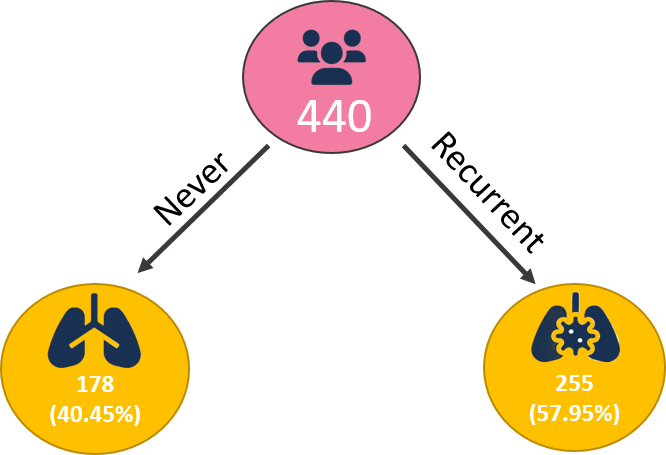
\includegraphics[width=\textwidth]{Figures/Chp3_data.png}
            \end{figure}
        \column{.5\textwidth}
        \small
        \begin{itemize}
            \item Censor at death/lung transplant/pregnancy
            \item Review year 2003+
            \item Age 6+ years
            \item Num obs. 3+ spanning 6+ months
            \item Random 6 centers by lung severity
            \item Sample size 440 patients
        \end{itemize}
    \end{columns}
\note{In this section, we will check joint model performance in our motivating data. The bullets on the right panel are some key inclusive criteria that result in a total of 440 patients from 6 centers, of which about 40\% patients never experience PEx, while 58\% patients experience the recurrent events during the follow-up period.}
\end{frame}


\begin{frame}{Motivating Data (cont'd)}
    \begin{table}[H]
    \caption{\scriptsize Model comparisons with the boldface as the smallest LOOIC}  \vspace{-5mm}
    \resizebox{\columnwidth}{!}{
        \begin{threeparttable}
            \begin{tabular}{l|l|l|l|l}
            \toprule
            Association + Risk scale & Model & $\mbox{LOOIC}$ \tnote{a} (SE\tnote{b} )  & $\mbox{LOOIC}_1$\tnote{c} (SE\tnote{b} ) & $\mbox{LOOIC}_2$\tnote{d} (SE\tnote{b} ) \\ \hline
            \multirow{2}{*}{Slope + Gap} & Joint Model &  52551.9 (383.1) &	52490.3                                                 (231.5) &  61.6 (151.6) \\
                             & Two-stage Model & 52578.8 (385.7) &	52460.9 (232.3) & 117.9 (153.4)               \\ \hline
            \multirow{2}{*}{Slope + Calendar} & Joint Model & 52563.0 (389.4) & 52473.1 (231.9) & 89.9 (157.5) \\
                                  & Two-stage Model & 52575.5 (390.2) & 52460.9 (232.3) & 114.6 (157.9) \\ \hline
            \multirow{2}{*}{Value + Gap} & Joint Model & 52574.8 (383.4) & 52491.1 (230.6) & 83.7 (152.8)\\ 
                                         & Two-stage Model & 52602.4 (384.5) & 52460.9 (232.3) & 141.5 (152.2)
                                                        \\ \hline
            \multirow{2}{*}{\textbf{Value + Calendar}} & \textbf{Joint Model} &                     \textbf{52537.3 (386.2)} &                                                            52486.4 (231.1) & 50.9 (155.1) \\ 
                                             & Two-stage Model & 52551.3 (388.3) &	52460.9 (232.3) & 90.4 (156)\\
            \bottomrule
            \end{tabular}
        \begin{tablenotes}[para]
        \footnotesize
        \item[a] Joint model; \item[b] Standard error approximated as byproduct of \emph{loo} package; \item[c] Longitudinal submodel; \item[d] Event submodel
        \end{tablenotes}
    \end{threeparttable}}
    \end{table}
\note{We examine a total of eight models, including joint models and two-stage models under difference scenario. We note that all joint models are preferred than the corresponding two-stage approaches with smaller LOOIC. From the statistical sight, the joint model with current value as the association structure in a calendar time scale outperforms others by the lowest LOOIC. Nonetheless, the choice between calendar or gap time also depends on clinical interests and some other combinations of risk factors. But for illustration purpose, we pick the 'optimal' model from statistical perspective here.}
\end{frame}

\begin{frame}
\frametitle{Motivating Data (cont'd)}
\begin{itemize}
    \item \textbf{Longitudinal outcome: ppFEV1}
    \begin{itemize}
        \item Positive: baseline ppFEV1; num PEx within prior year, birth cohort, male
        \item Negative: time, $\mbox{time}^2$, pa
    \end{itemize}
    \item \textbf{Time-to-recurrent outcome: PEx}
    \begin{itemize}
        \item Positive: num previous PEx
        \item Negative: baseline insurance, male
    \end{itemize}
    \item \textbf{Association structure}
    \begin{itemize}
        \item one percentage predicted \textcolor{red}{increase} in ’true and unobserved’ ppFEV1 would \textcolor{red}{decrease} PEx risk for 
         \begin{multicols}{3}
            \begin{itemize}
                  \item Center 1: 3.92\%
                  \item Center 4: 3.92\%
                  \item Center 2: 4.88\%
                  \item Center 5: 2.96\%
                  \item Center 3: 3.92\%
                  \item Center 6: 3.92\%
            \end{itemize}
        \end{multicols}
    \end{itemize}
\end{itemize}
\note{Again, risk factors are selected from STEPWISE algorithm from the preliminary analysis. Their positive and negative impacts are briefly summarized here. We not only observe the negative association between ppFEV1 and PEx, but also we are able to quantify the center-specific association as interpreted here, which will greatly facilitate the further inference. }
\end{frame}


\begin{frame}{Motivating Data (cont'd)}
    \begin{figure}[H]
    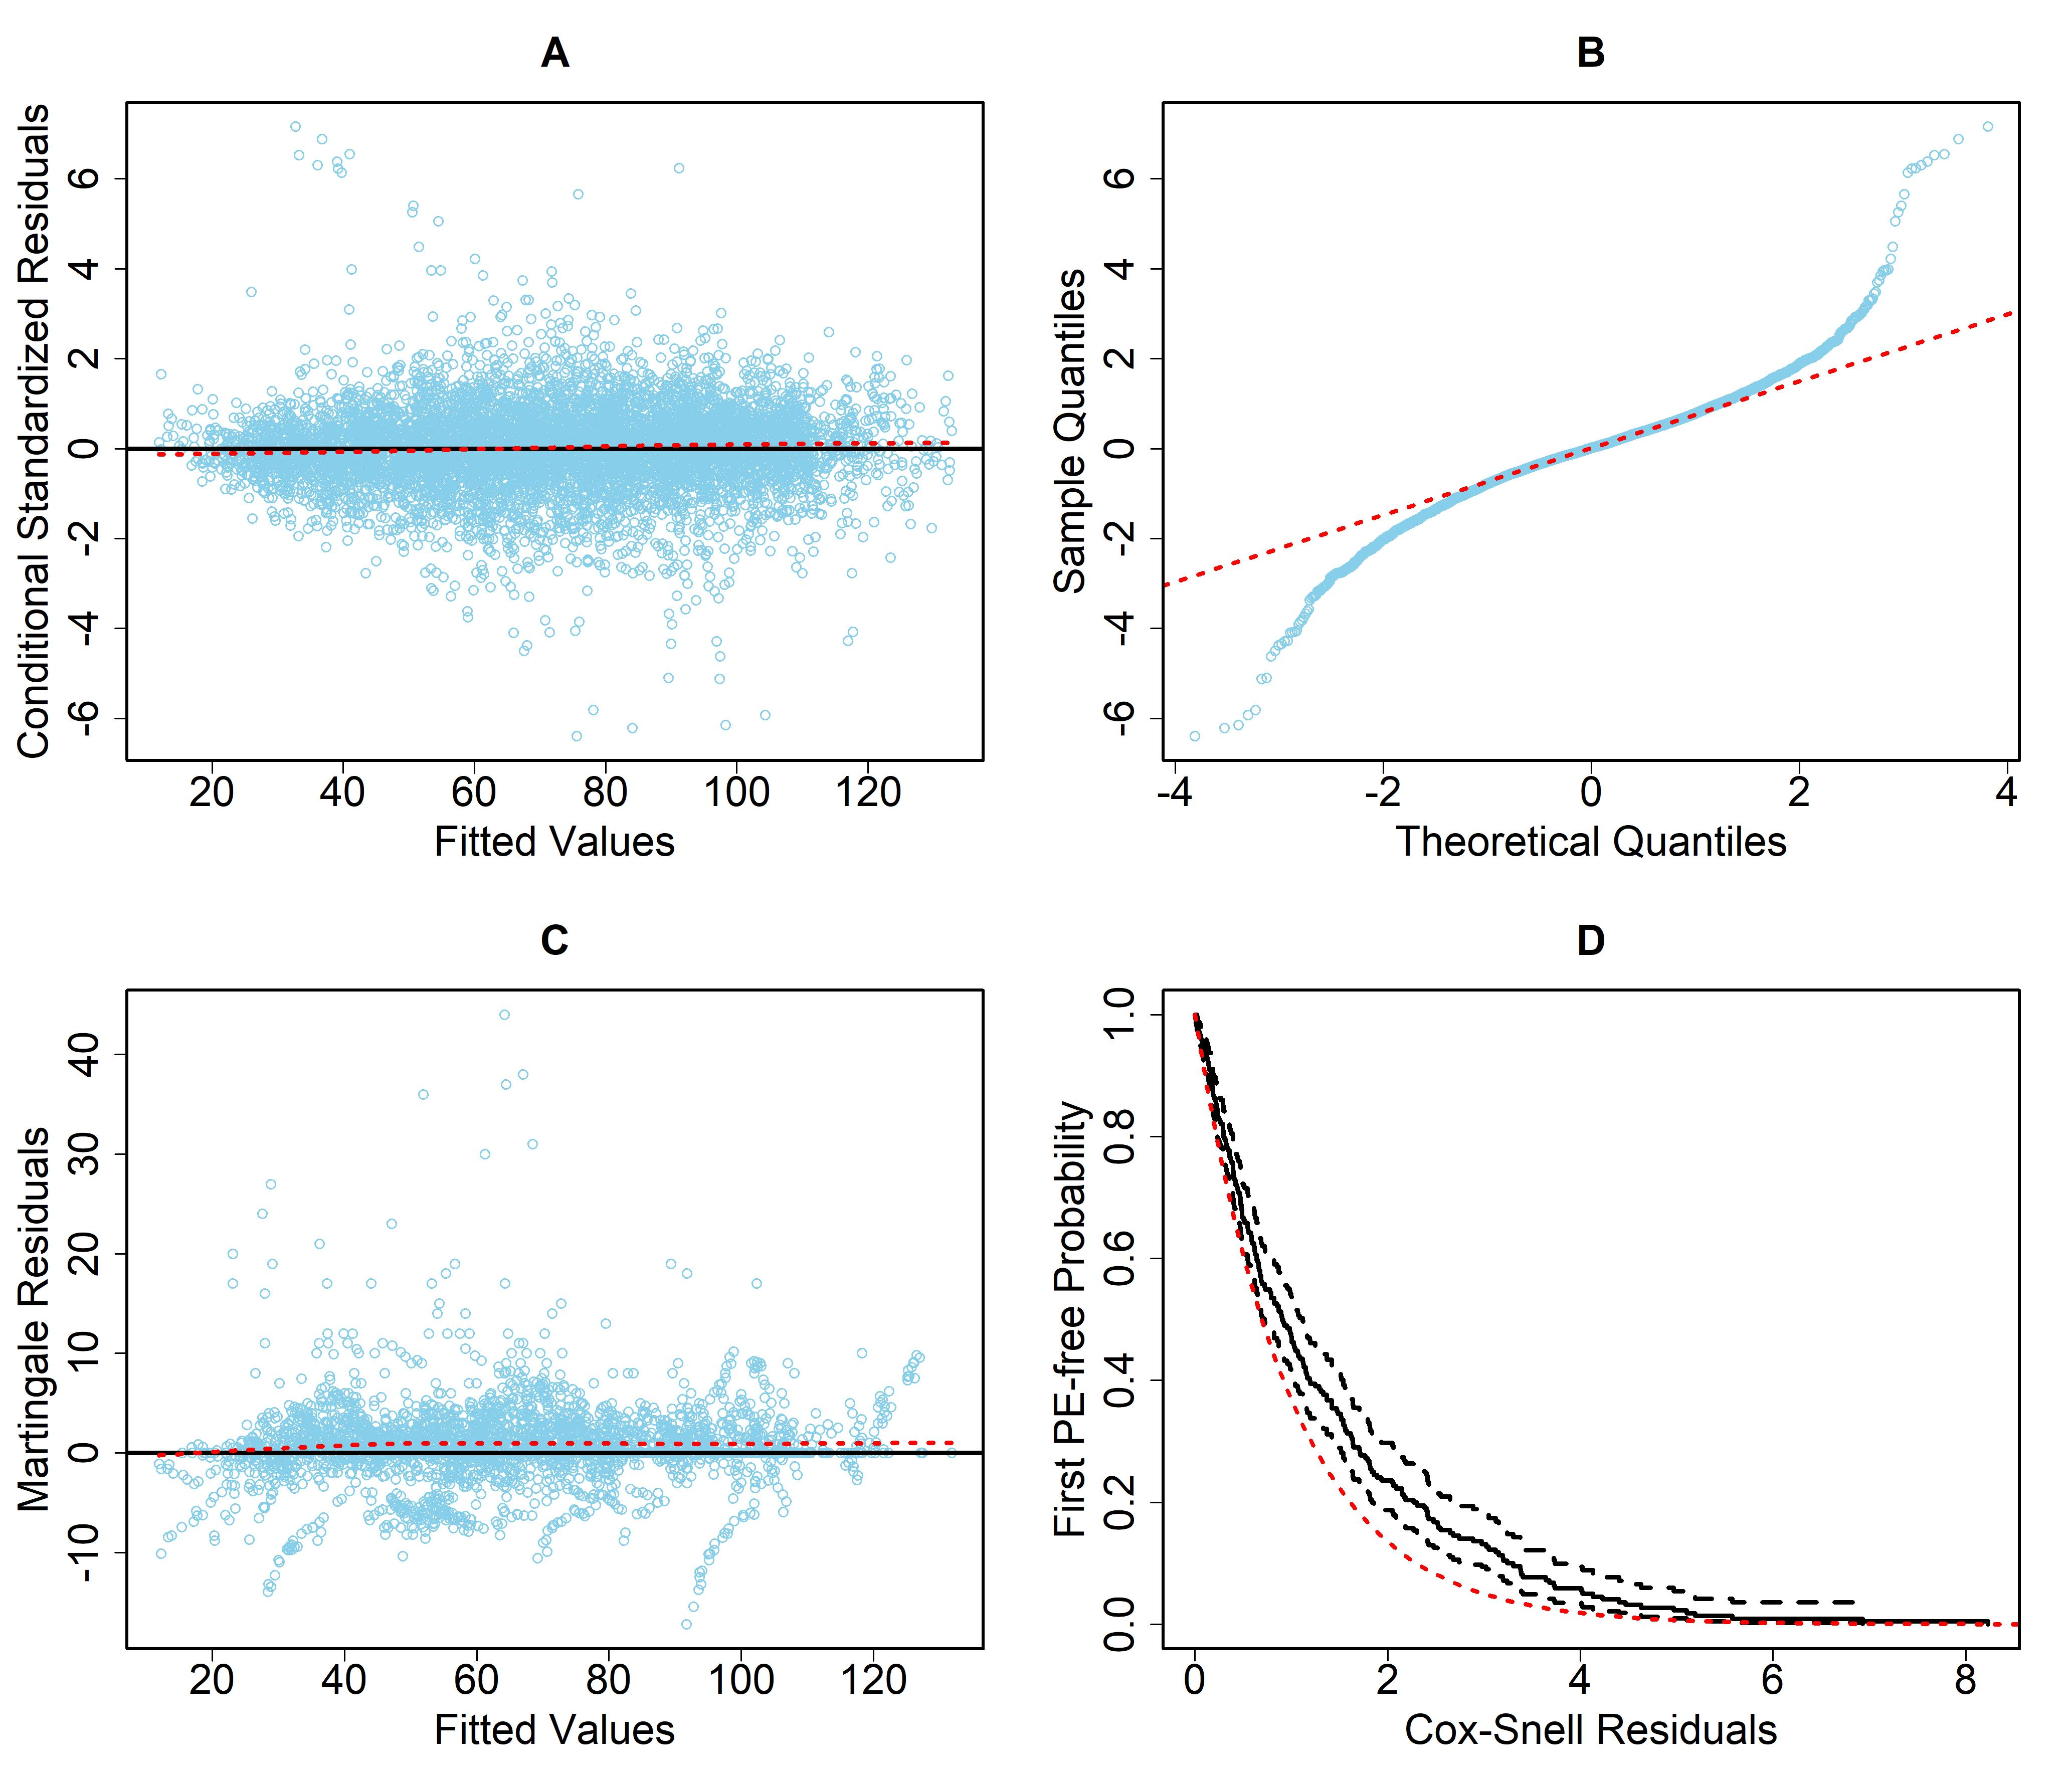
\includegraphics[width=0.65\textwidth]{Figures/Chp3_DIAG.jpg}
    \caption{\tiny (A) subject-specific standardized residuals versus fitted values; (B) normal Q-Q plot; (C) subject-specific martingale residuals versus fitted values; (D) Cox-Snell residuals. Red dashed lines: loess curve (A \& C); normal curve (B); exponential curve (D)}
    \end{figure}
\note{We also check the diagnostics for the optimal joint model through basic residual tools. Plot A and B are for the longitudinal submodel, it looks good despite some heavier tail behavior. Plot C and D are for the event submodel, again, no striking violations are found.}
\end{frame}

\begin{frame}{Motivating Data (cont'd)}

    \begin{table}[H]
        \caption{\scriptsize Predictive performance of proposed joint models}
        \scriptsize
            \begin{threeparttable}
                \begin{tabular}{c|c|c|c|l|c|c}
                \toprule
            $t_{li}$ & $\Delta t$ & $t'$ & Num at risk & Joint Model & AUC & MPE \\ \hline
        \multirow{4}{*}{$[0,2.73)$}
        &\multirow{4}{*}{1.41} &\multirow{4}{*}{2.73} &\multirow{4}{*}{42} & Slope + Gap & 0.61 & 0.28 \\
        &&&& Slope + Calendar & 0.64 & 0.27 \\
        &&&& Value + Gap & 0.66 & 0.27 \\
        &&&& Value + Calendar & 0.68 & 0.26 \\ \cline{1-7}
        \multirow{4}{*}{$[0, 5.10)$} &\multirow{4}{*}{1.56} &\multirow{4}{*}{5.10} & \multirow{4}{*}{65} & Slope + Gap & 0.89 & 0.14 \\
        &&&& Slope + Calendar & 0.88 & 0.14 \\
        &&&& Value + Gap & 0.90 & 0.14 \\
        &&&& Value + Calendar & 0.88 &	0.14\\ \cline{1-7}
        \multirow{4}{*}{$[0, 7.84)$} &\multirow{4}{*}{2.76} &\multirow{4}{*}{7.84} & \multirow{4}{*}{31} & Slope + Gap & 0.92 &	0.12 \\
        &&&& Slope + Calendar & 0.91 & 0.13 \\
        &&&& Value + Gap & 0.92 &	0.12 \\
        &&&& Value + Calendar & 0.92 & 0.13\\ 
                \bottomrule
                \end{tabular}
        \begin{tablenotes}[para]
        \tiny
        Note: t=individual prediction start time in year; $\Delta t$: averaged prediction window in year; $t'$: future time in year; Num at risk: Number of patients at risk at $t'$; AUC=area under curve; MPE=mean predictive error based on squared loss function
        \end{tablenotes}
    \end{threeparttable}
    % }
    \end{table}
\note{To assess predictive performance, we predict from the individual start time to a common future time $t'$. We observe that all joint models show reasonable predictive accuracy. As time elapsed, more time-varying covariates become available, thus facilitate the predictive performance in the longer term run.}
\end{frame}


\begin{frame}{Motivating Data (cont'd)}
    \begin{figure}[H]
    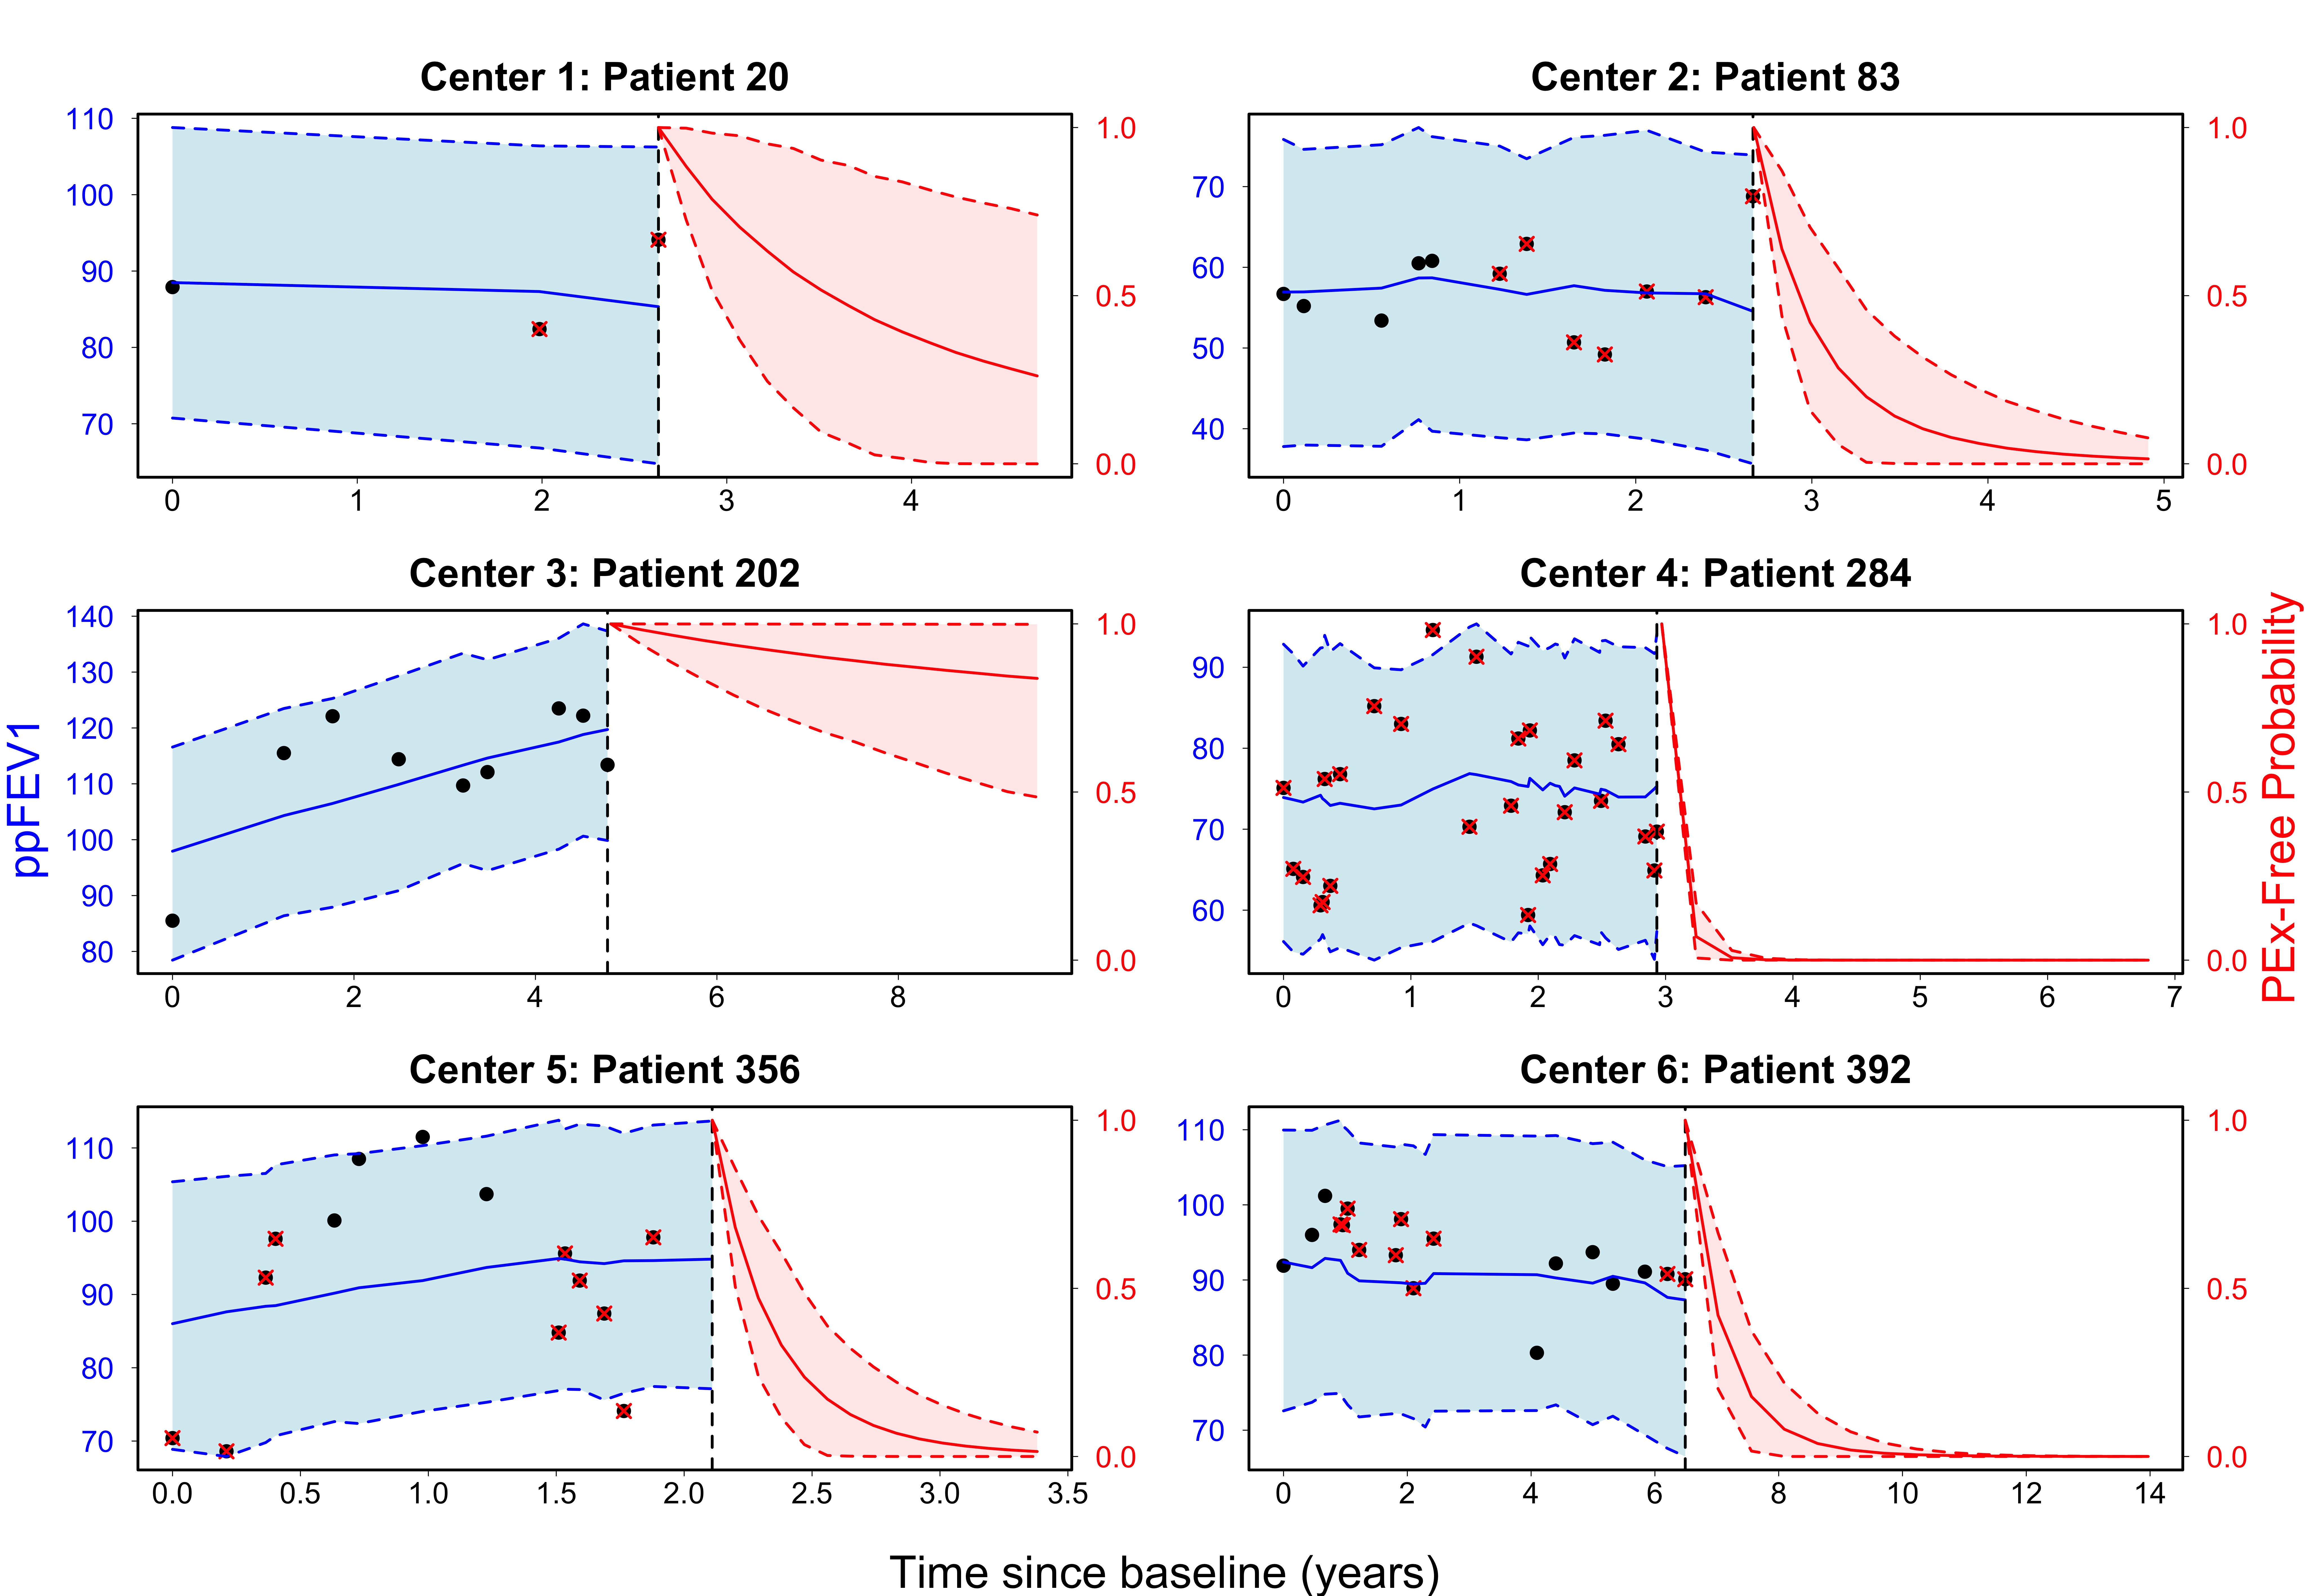
\includegraphics[width=0.9\textwidth]{Figures/Chp3_PRED_PLOT2.jpg}
    \end{figure}
\note{We plot for 6 random patients who are still at risk after the last observed measurement, including observed historical ppFEV1 in dots with marked PEx events. Fitted ppFEV1 values are in blue and predictive probabilities are in red. Both with 95\% highest posterior density intervals. We observe that Patient 202 and Patient 284 represent two extreme cases, suggesting that higher lung function reduces the risk of the next PEx event, while the latter patient needs a timely prevention given super high probability of PEx. 
% Also, we observe that averaged value of ppFEV1 and the frequency of previous PEx events might be important risk factors for the the next PEx event.
}
\end{frame}

\begin{frame}{Discussion}
\begin{itemize}
    \item \textbf{Features}
    \begin{itemize}
        \item Time-to-recurrent events in two risk scales
        \item Center-specific time-dependent association structure 
        \item Applicable Stan programs
        \item Joint model diagnostics
    \end{itemize}
   
    \item \textbf{Extensions}
    \begin{itemize}
        \item Presence of terminal event
        \item Dynamic individual prediction
        \item Alternative baseline hazard candidates
    \end{itemize}
\end{itemize}
\note{To conclude for this project, we fill the methodological gap for the \textbf{multilevel} joint model of longitudinal and recurrent outcomes. We demonstrate two risk scales and develop the center-specific time-dependent association structure between two processes. We also implement the applicable Stan programs for reproduction. Lastly, we investigate joint model diagnostics, which has not received much attention in the joint modeling literature. There are some interesting extensions can be studied: i) we can add an extra submodel for the terminal event; ii) extend our predictive rationale for dynamic individual prediction; iii) replace current Weibull baseline hazard with some other flexible candidates.}
\end{frame}

\section[Conclusion]{Conclusion and Future Work}
\setcounter{subsection}{1}

\begin{frame}
\frametitle{}
\begin{enumerate}
    \item<0> \textbf{Introduction}
    \item<0> \textbf{Multilevel Bayesian Joint Model of Longitudinal and Binary Outcomes}
    \begin{itemize}
        \item Motivation
        \item Model framework
        \item Simulation study \& Motivating data
        \item Discussion
    \end{itemize}
    \item<0> \textbf{Multilevel Bayesian Joint Model of Longitudinal and Recurrent Outcomes}
    \begin{itemize}
        \item Motivation
        \item Model framework
        \item Simulation study \& Motivating data
        \item Discussion
    \end{itemize}
    \item \textbf{Conclusion and Future Work}
\end{enumerate}
\end{frame}

\begin{frame}
\frametitle{Conclusion}
\begin{itemize}
    \item Two novel multilevel Bayesian joint models for PEx risk in hierarchically structured data
    \begin{itemize}
        \item PEx as binary outcome: Gaussian process + Flexible link
        \item PEx as recurrent outcome: Current value + Calendar time
    \end{itemize}
    \item Rationale for (dynamic) individual prediction
    \item Center-specific association strength
    \item Applicable Stan programs \& R codes (\footnotesize \href{https://github.com/GraceChenZhou/2022\_DISSERTATION.git}{\textcolor{blue}{https://github.com/GraceChenZhou/2022\_DISSERTATION.git}})
    
\end{itemize}
\note{To summarize, we have proposed two novel multilevel Bayesian joint models in hierarchically structured data, which both present reasonable personalized prediction for the PEx risk. Specifically, in the 1st project, we account for PEx as the longitudinal binary outcome and we are interested in the occurrence of PEx and in the 2nd project, we take PEx as the recurrent outcome so that we are interested in the time to next recurrent event. The different motivation result in different submodel frameworks, but we apply center-specific association parameter to both projects, which greatly facilitate the model performance. The Stan and R codes are open source that can be found from my Github to inspire researchers with similar data set and objective.}
\end{frame}


\begin{frame}
\frametitle{Future Work}
\begin{itemize}
    \item RShiny app
    \item Left-truncation problem
    \item parallel-HMC algorithm
\end{itemize}
\note{To make our joint model more applicable to the public, we are now programming the RShiny app that can incorporate dynamic individual prediction and some other functions. Also given the feature of our registry data, there exists left-truncation problem, therefore we can study the remedy in the future. To reduce the cost of intensive computational time, we can investigate some parallel computation techniques. 
% The algorithm firstly partitions data into multiple subsets and independently runs MCMC sampler, then applies random partition trees to combine all posterior draws.  
}
\end{frame}

\begin{frame}{Acknowledgements}
\begin{itemize}
    \item Advisor: Dr. Seongho Song
    \item Co-advisor: Dr. Rhonda D. Szczesniak
    \item Committee Members: Dr. Won Chang, Dr. Joon Hang Kim and Dr. Xia Wang    
\end{itemize}
\note{My sincere thanks go to my advisor, co-advisor and all committee members.}
\end{frame}


\section[Appendix]{Appendix}
\setcounter{subsection}{1}
\begin{frame}
\frametitle{}
\begin{center}
\textbf{\Large Appendix}
\end{center}
\end{frame}

\begin{frame}{LKJ correlation distribution}
\small
\begin{itemize}
    \item $lkjCorr(\Sigma|\eta) \propto det(\Sigma)^{\eta-1}$ 
    \item $\Sigma$ is a positive-definite, symmetric matrix with unit diagonal correlation matrix (i.e., a correlation matrix) with shape parameter $\eta \in \mathbb{R}^+$ (\cite{Lewandowski2009})
    \item Practically, \emph{Stan} provides an implicit parameterization of the LKJ correlation matrix density in terms of its Cholesky factor
    \begin{itemize}
          \item Let $L_u$ denote a Cholesky factor of the correlation matrix $\Sigma=\begin{pmatrix}
    1 & \rho \\
    \rho & 1
    \end{pmatrix}$
        \item $L_u \sim \mbox{lkj\_corr\_cholesky}(2)$ implies $\Sigma = L_u \cdot L^{T}_u \sim lkjCorr(2)$
    \end{itemize}
\end{itemize}

\end{frame}

\begin{frame}{Conditional Survival Probability}
\tiny
    \begin{flalign}
 S_{li}(t'|t) & = p(t_{n_{li}+1} \geq t'|t_{n_{li}+1} > t,\mathcal{D})&&\\\nonumber
              & = \int\int\int\int p(t_{n_{li}+1} \geq t'|t_{n_{li}+1} > t, b_l,\bm{U}_{li},v_{li},\bm{\theta},\mathcal{D})p(b_l, \bm{U}_{li}, v_{li}, \bm{\theta} |t_{n_{li}+1} > t, \mathcal{D}) db_l \, d\bm{U}_{li} \, dv_{li} \, d\bm{\theta}&& \nonumber \\
              & = \int\int\int\int \frac{p(t_{n_{li}+1} \geq t'|b_l, \bm{U}_{li}, v_{li}, \bm{\theta})}{p(t_{n_{li}+1} > t|b_l, \bm{U}_{li}, v_{li}, \bm{\theta})} \cdot p(b_l, \bm{U}_{li}, v_{li}, \bm{\theta} |t_{n_{li}+1} > t, \mathcal{D}) \, db_l \, d\bm{U}_{li} \, dv_{li} \, d\bm{\theta}&& \nonumber \\
              & = \int\int\int\int \frac{S(t'|b_l, \bm{U}_{li}, v_{li}, \bm{\theta})}{S(t|b_l, \bm{U}_{li}, v_{li}, \bm{\theta})} \cdot p(b_l, \bm{U}_{li}, v_{li}, \bm{\theta} |t_{n_{li}+1} > t, \mathcal{D}) \, db_l \, d\bm{U}_{li} \, dv_{li} \, d\bm{\theta}&& \nonumber \\
              &=\int\int\int\int \frac{exp\Big[-\int_{0}^{t'}h(s|b_l, \bm{U}_{li}, v_{li}, \bm{\theta})ds\Big]}{exp\Big[-\int_{0}^{t}h(s|b_l, \bm{U}_{li}, v_{li}, \bm{\theta})ds\Big]} \cdot p(b_l, \bm{U}_{li}, v_{li}, \bm{\theta} |t_{n_{li}+1} > t, \mathcal{D}) \, db_l \, d\bm{U}_{li} \, dv_{li} \, d\bm{\theta}&& \nonumber \\
              &=\int\int\int\int exp\Big[-\int_{t}^{t'}h(s|b_l, \bm{U}_{li}, v_{li}, \bm{\theta})ds\Big] \cdot p(b_l, \bm{U}_{li}, v_{li}, \bm{\theta} |t_{n_{li}+1} > t, \mathcal{D}) \, db_l \, d\bm{U}_{li} \, dv_{li} \, d\bm{\theta}&& \nonumber \\
              & \approx \frac{1}{M} \sum_{m=1}^{M} exp\Big[ -\int_t^{t'} h\big(s|b_l^{(m)},\bm{U}_{li}^{(m)},v_{li}^{(m)},\bm{\theta}^{(m)}\big) ds \Big] \nonumber
\end{flalign}
\end{frame}

\begin{frame}{Time-dependent AUC}
\begin{table}[H]
\scriptsize
\resizebox{\columnwidth}{!}{
\begin{tabular}{p{14cm}} 
 \toprule
 \textbf{Time-dependent AUC}\\
 \midrule
  \begin{enumerate}
      \item Define individual-specific start time $t_i=\mbox{tstart}_i$ and a common future stop time $t'$. To conform the prediction data, we only include individuals who are still at risk of the event at $t$. For longitudinal data, we adopt observations observed until $t_i$. 
      \item Calculate event-free ('survival') probability at $t'$ and observed $\mbox{tstop}_i$ for each individual based Equation (\ref{eq:cond.surv}) to obtain $S_i(t'|t_i)$ and $S_i(\mbox{tstop}_i|t_i)$
      \item Sort individuals by their observed $\mbox{tstop}$ in an increasing order and group each two by combinations without replacement. 
      \item AUC is calculated by accounting for weights caused by censoring conditions. For each combation $c=1,\dots,C$, assume that $\mbox{tstop}_i < \mbox{tstop}_j$:
        \begin{itemize} \scriptsize
            \item If only individual $i$ is censored at $t'$, which means $\mbox{tstop}_i \leq t'$ \& $\mbox{status}_i=0$, then weight $w=1-S_i(\mbox{tstop}_i|t_i)$
            \item If only individual $j$ is censored at $t'$, which means $\mbox{tstop}_j \leq t'$ \& $\mbox{status}_j=0$, then weight $w=S_j(\mbox{tstop}_j|t_j)$
            \item If both individuals are censored at $t'$, then weight $w=\big(1-S_i(\mbox{tstop}_i|t_i)\big) \times S_j(\mbox{tstop}_j|t_j)$
            \item If it does not belong to above cases, $w=1$
            \item Let $S_i=S_i(t'|t_i), S_j=S_j(t'|t_j)$, compute $A_c=I_{S_i<S_j} \cdot w$; $D_c=I_{S_i>S_j} \cdot w$; $T_c=I_{S_i=S_j} \cdot w$, where $I_x$ denotes a indicator function with 1 when $x$ is true and 0, otherwise. 
        \end{itemize}
      \item Repeat Step 4 until $C$ times
      \item $\mbox{AUC}=\sum_{c=1}^C \big(\frac{A_c+0.5 \cdot T_c}{A_c + D_c + T_c}\big)$
  \end{enumerate}\\
 \bottomrule
 \hline
\end{tabular}}
\end{table}
\end{frame}

\begin{frame}{Time-dependent MPE}

\begin{table}[H]
\scriptsize
\resizebox{\columnwidth}{!}{
\begin{tabular}{p{14cm}} 
 \toprule
 \textbf{Time-dependent mean predictive error (MPE)}\\
 \midrule
   \begin{enumerate}
     \item  For each individual $i (i=1,\dots,N)$: 
         \begin{itemize} \scriptsize
             \item If individual $i$ died or censored after $t'$, $\mbox{Error}_i=(1-S_i)^2$
             \item If individual $i$ died before $t'$, $\mbox{Error}_i=(0-S_i)^2$
             \item If individual $i$ censored before $t'$, $\mbox{Error}_i=S_i(\mbox{tstop}_i|t_i) \times (1-S_i)^2+\big(1-S_i(\mbox{tstop}_i|t_i)\big) \times (0-S_i)^2$
         \end{itemize}
    \item Mean Predictive Error (MPE)=$\frac{\sum_{i=1}^{N}\mbox{Error}_i}{N}$
 \end{enumerate}\\
 \bottomrule
\end{tabular}}
\end{table}
\end{frame}

\begin{frame}{Project I: System \& Time}
\tiny
\begin{table}[H] 
\resizebox{\columnwidth}{!}{
 \begin{threeparttable}
\begin{tabular}{c|c|c|c}
\toprule
 & \bf Mac & \bf PC & \bf BMI\\
\hline
Platform & x86\_64-apple-darwin17.0 (64-bit) & x86\_64-w64-mingw32/x64 (64-bit) & x86\_64-pc-linux-gnu\\
\hline
Running under & macOS Big Sur 10.16 & Windows 10 x64 (build 19043) & x86\_64, linux-gnu\\
\hline
R version & 4.0.5 (2021-03-31) & 4.0.2 (2020-06-22) & 3.6.1 (2019-07-05) \\
\hline
CmdStan & v2.28.2 & v2.29.1 & - \\
cmdstanr & v0.4.0 & v0.5.0 & - \\ 
rstan & - & - & 2.19.2 \\
\bottomrule
\end{tabular}
  \begin{tablenotes}[para]
    \tiny
   Note: i). Simulation A: Mac \& PC; ii) Simulation B \& Real data: Biomedical Informatics (BMI) at CCHMC
    \end{tablenotes}
 \end{threeparttable}}
\end{table}

\begin{table}[H] 
     \resizebox{\columnwidth}{!}{
    \begin{threeparttable}
    \begin{tabular}{l|l|c|c|c}
    \toprule
    Joint Model & Flexible link & Simulation A (mins/rep) & Simulation B (hrs/rep) & Motivating Data (hrs/rep)\\ \hline
    \multirow{2}{*}{JM1} & splogit  & - & 0.20 & -\\
                         & spep     & - & 0.16 & 1.42\\ \hline
    \multirow{2}{*}{JM2} & splogit  & - & 0.25 & -\\
                         & spep     & - & 0.22 & 2.86 \\ \hline
    \multirow{2}{*}{JM3} & splogit  & 0.31 & 0.19 & -\\ 
                         & spep     & - & 0.18 & 7.62 \\ \hline
    \multirow{2}{*}{JM4} & splogit  & - & 0.61 & - \\              
                         & spep     & - & 0.70 & 13.7\\
    \bottomrule
    \end{tabular}
    \begin{tablenotes}[para]
    \tiny
   mins=minutes; rep=replicate; hrs=hours
    \end{tablenotes}
     \end{threeparttable}}
\end{table}
\end{frame}

\begin{frame}{Project II: System \& Time}
\tiny
\begin{table}[H] 
\begin{tabular}{c|c|c}
\toprule
 & \bf Simulated data & \bf Real data\\
\hline
Platform & x86\_64-apple-darwin17.0 (64-bit) & x86\_64-w64-mingw32/x64 (64-bit)\\
\hline
Running under & macOS Big Sur 10.16 & Windows 10 x64 (build 19043)\\
\hline
R version & 4.0.5 (2021-03-31) & 4.0.2 (2020-06-22) \\
\hline
CmdStan & v2.28.2 & v2.29.1 \\
cmdstanr & v0.4.0 & v0.5.0\\ 
\bottomrule
\end{tabular}
\end{table}

\begin{table}[H] 

\begin{threeparttable}
\begin{tabular}{l|l|c|c}
\toprule
Association + Time scale & Model & Simulated data (hrs/rep) & Real data (hrs) \\ \hline
\multirow{2}{*}{Slope + Gap} & Joint Model &  0.18 & 9.16\\
                             & Two-stage Model & 0.05 & 2.86\\ \hline
\multirow{2}{*}{Slope + Calendar} & Joint Model & 0.26 & 3.82\\
                                  & Two-stage Model & 0.08 & 2.59 \\ \hline
\multirow{2}{*}{Value + Gap} & Joint Model & 0.18 & 8.17\\ 
                             & Two-stage Model & 0.04 & 5.31 \\ \hline
\multirow{2}{*}{Value + Calendar} & Joint Model & 0.15 & 7.10 \\              
                                           & Two-stage Model & 0.04 & 4.90\\
\bottomrule
\end{tabular}
 \begin{tablenotes}[para]
 \tiny
  rep=replicate; hrs=hours
    \end{tablenotes}
 \end{threeparttable}
\end{table}
\end{frame}


\begin{frame}[allowframebreaks]
\frametitle{References}
\tiny
\bibliographystyle{apalike}
\bibliography{ref}
\end{frame}


\end{document}